\chapter{Cross-tissue comparison of chromatin accessibility, gene expression signature and immunophenotypes in PsA}
\chaptermark{Cross-tissue comparison analysis in PsA}
\label{ch:Results3}


%%%%%%%%%%%%%%%%%%%%%%%%%%%%%%%%%%%%%%%%%%%%%%%%%%

\section{Introduction}

\subsection{The relevance of cell type and tissue specificity in the study of PsA}

Consideration of cell and type specificity in the study of complex diseases is fundamental for the understanding of the disease pathophysiology. As previously reviewed (\ref{ch:Intro}), the dysregulated immune response in PsA is the results of the interaction between cellular components of the innate and adaptive immune response. Consequently, the molecular characterisation of the different immune cell types is pivotal not only for the understanding of the immune response but also to define disease state, comprehend the impact of genetic variants increasing disease risk and identify drugs with optimal efficacy and specificity.


\subsubsection{Differences in the PsA inflammatory response between blood and the synovium}

PsA is considered a systemic disease where studies in PBMCs have demonstrated changes in cell type composition and cytokine production when compared to healthy individuals. For example, increased frequencies of circulating IL-17$^+$ and IL-22$^+$ CD4$^+$ T cells have been reported in PB from PsA patients compared to control individuals \parencite{Benham2013}. Moreover, reduced percentage of pDCs and NK in PB have also been observed in PB from PsA compared to controls \parencite{Jongbloed2008, Spadaro2004}. In terms of cytokine production, stimulated PBMCs from PsA patiens released greater levels of IL-17 and IL-22 than the healthy control counterparts \parencite{Benham2013}. 
Nevertheless, PsA is characterised by affection of the joints, where the local inflammatory response leads eventually to joint destruction. Oligoarticular PsA (involving four or fewer joints) is commonly managed by joint aspiration prior intra-articular steroid injection to relieve pain, facilitating the sample collection for research purposes \parencite{Kavanaugh2006}. The importance of studying the synovium in PsA have been highlighted by differences in cell composition and cytokine production, amongst others, between PB and SF in PsA patients. For example, expansion mCD8$^+$ but not mCD4$^+$ T cells was observed in SF when compared to PB in PsA paired samples \parencite{Ross2000}. Additionally, elevated proportion of T cells expressing the cytokine receptors CCR6$^+$ and IL-23R$^+$ were found in SF compared to PB in patients \parencite{Benham2013}.


\subsection{Bulk transcriptomic studies and their limitations}

Genome-wide transcriptomic studies in PsA have been mainly focused in characterising gene expression in bulk PBMCs and SFMCs samples. Several studies have been conducted to better understand gene expression differences in blood between PsA and controls and also specific differences between PB and SF from the same PsA patients or differences with other arthritic diseases \parencite{Stoeckman2006, Batiwalla2005, Gu2002, Dolcino2015}. Amongst the most comprehensives of thesestudies, that conducted by Dolcino and colleagues revealed genes from the Th-17 axis and type-I IFN signalling to be differentially expressed between PsA and healthy controls in synovial membranes. Moreover, the overlapof genes that were differentially expressed betweenpatients and controls in each of the compartments, highlighted differences and commonalities in the systemic and synovial immune response in PsA. %Other studies have also focused in the understanding the transcriptional changes in PBMCs from PsA patients following MTX and TNFi therapies \parencite{Cuchacovich2014}. 
Cytokines production measurements have also been conducted in serum and SF, revealing increased levels of TNF-$\alpha$, for example, in both tissues \parencite{Ritchlin1999,Li2017}. 

Studies using mixed cell populations can be influenced by the relative proportion of the different cell populations within the sample \parencite{Whitney2003}. For instance, the importance of considering cell types to understand the impact of genetic variants in transcriptional regulation has been explored in a number of immune cells \parencite{Fairfax2012, Fairfax2014, Raj2014, Peters2016, Kasela2017}. These studies have highlighted the regulatory role of some genetic variants only in particular cell types and conditions, previously masked when considering mixed population of cells such as PBMCs. In this respect, expression analysis for a limited number of genes have been performed in specific cell type populations such as stimulated macrophages and Th-17 \textit{in vitro} differentiated cells from na\"{i}ve CD4$^+$ isolated from PB and SF of PsA patients \parencite{Antoniv2006, Leipe2010}. Overall, achieving a detailed and precise understanding of complex diseases requires the study of sorted cell populations and when possible isolated from the affected tissue.  


\subsection{Transcriptomics and proteomics at the single cell resolution}

In addition to the study of specific cell types, evidence for heterogeneity in the transcriptome across individual cells from the same population has accelerated the development of strategies providing single cell resolution. The establishment of scRNA-seq and mass-cytometry techniques represent an unbiased way to characterise and identify cell subpopulations within the samples, avoiding the pre-selection of particular cell types and thus providing a global overview of cell composition and interactions in the tissue of interest. 

A wide range of approaches to study single-cell transcriptomics have been developed in the last few years, including Drop-seq, SmartSeq2 and 10X Chromium amongst the most widely used \parencite{Picelli2014,Ziegenhain2017}. 10X Chromium technology is based on microfluidics where cells in suspension get directly encapsulated into nanoL droplets that incorporate cell and transcript barcode identifiers (see \ref{ch:Mat}). As a result, 10X Chromium technology does not require pre-sorting of single-cells into plates and enables higher throughput than other with less manipulation and variability than other scRNA-seq methods such as SmartSeq2 \parencite{Baran-Gale2017}.
 
Mass cytometry represents the next generation of fluorescence based flow-cytometry analysis to interrogate expression of cell surface and intracellular molecules. Mass cytometry is a hybrid technique between mass spectrometry and flow cytometry, where the Abs recognising the molecular markers have been labelled with stable isotopes instead of fluorophores \parencite{Bandura2009}. The use of isotopes enables incorporating up to 45 Abs to profile cellular populations and assess molecular functions. 



\subsection{Using a multi-omics approach in the study of complex diseases}

The interaction between genetics and environmental factors in the risk to develop complex diseases, such as PsA, results in shaping the epigenetic landscape of the cells. This dynamism of the  epigenome involves cell and context specific features, reinforcing the importance of studying purified cell types instead of mixed populations. Moreover, the importance of the epigenomic landscape in understanding disease state and also contextualizing the role of putative genetic risk variants has made necessary the implementation of multi-omics approaches to study complex diseases. This involves the study of chromatin accessibility, gene expression including further resolution using scRNA-seq and immunophenotypes of the relevant cell involved in disease pathophysiology.

%Recent technical advances such as ATAC-seq are enabling the characterisation of the regulatory landcape in a wide range of cell types and tissues obtained from valuable clinical samples minimising the amount of material required. Profiling the chromatin accessibility in the cell populations isolated from the tissues of interest provides details about the molecular programming of cells and can also inform about the location and status of \text{cis}-regulatory elements. For example differential analysis in B cells isolated from SLE and healthy controls has revealed changes in chromatin accessibility for loci nearby genes involved in B cells activation and enrichment for TFBS potentially regulating pathogenic processes \parencite{Scharer2016}. Similarly a study in age-related macular degeneration (AMD) has identified the retina epithelium as the main tissue driving disease onset though global loss of chromatin accessibility compared to healthy tissue \parencite{Wang2018}. 


%Short sentence to link to ATAC-seq
Transcriptional profiling of discrete cell populations have also been performed in monocytes and Th-17 cells in AS, intestinal epithelial cells in CD and fibroblast-like synoviocytes in RA \parencite{Al-Mossawi2017,Smith2008, Howell2018, Ai2016}. Moreover, recent advances have yielded the possibility to study the transcriptomic and proteomic profiles at the single-cell resolution and account for the variability at the single-cell level in gene expression and protein translation. 

Incorporation of scRNA-seq and mass cytometry in addition to bulk RNA-seq and flow cytometry have led to a more detailed understanding of the immune system \parencite{Jaitin2014, Villani2017,Bengsch2018}. In complex diseases such as RA, scRNA-seq has discovered heterogeneity in the synovial fibroblast population and identified a potentially pathogenic cluster highly proliferative and active in pro-inflammatory cytokine secretion \parencite{Mizoguchi2018}. Similarly, mass cytometry analysis performed in RA identified an expanded CD4$^+$ T cell population promoting B cell response \parencite{Rao2017}.

\subsubsection{Data integration}

One of the most challenging aspects of using a multi-omics approach is the appropriate integration of the data in order to maximise the amount of information extracted and also the reliability of the findings. The power of this integration is increased by generating paired data for all the omics across all the individuals in the cohort, which cannot always be achieved due to sample availability and cost.  
Integrating chromatin accessibility and gene expression data has allowed to better understand the correlation and specificity between open chromatin and transcription. In terms of identifying cell populations, chromatin accessibility has appeared to be more cell type specific than bulk RNA-seq \parencite{Corces2016}. In pancreatic islets, the overlap of ATAC-seq and RNA-seq has shown chromatin accessibility to be a better proxy for gene expression in $\alpha$ than in $\beta$ cells. Moreover, integration of both data sets reinforced the functional specificity of AMD DEGs nearby differentially accessible regions across tissues \parencite{Ackermann2016, Wang2018}. 

The most comprehensive available study integrating multi-omics (bulk RNA-seq, scRNA-seq and mass cytometry) has been performed in RA \parencite{Zhang2018}. This recent study has identified eighteen unique subpopulations amongst the the main cell types involved in RA pathophysiology by systematic correlation between transcriptional profiles and mass cytometry.

Regarding PsA, no such a comprehensive multi-omic study has been conducted to date. Characterisation of chromatin accessibility and transcriptomic landcape of the most relevant cell types in SF and PB would improve the understanding of differences across tissues as well as the relationship between chromatin accessibility and gene expression in PsA. Furthermore, implementation of single-cell transcriptomic and mass cytometry would help to  ......

%Example in PsA
 %For example, a genome-wide study of the methylome in PsA PBMCs revealed a hypomethylated pattern in na\"{i}ve patients compared to those under MTX treatment \parencite{Kim1996}. 


\subsection{Genetic fine-mapping using genotyping level data}
%Fine-mapping has been systematically applied to a number of immune-mediated GWAS, including T2D, IBD, AS and SLE \parencite{Maller2012,Gaulton2015,Bunt2015,Sun2016,Huang2017}. In contrast, systematic fine-mapping studies for all the sixty-three psoriasis GWAS loci have not been performed yet. In PsA, Bayesian fine-mapping has been conducted for some of the Immunochip GWAS associations, including the 5q31 PsA-specific locus  \parencite{Bowes2015}.
%
%% Maybe in the discussion
%Regardless the contribution towards dissecting causality, traditional Bayesian fine-mapping models assume only one causal SNP driving the association at each locus. As a way to partially address this limitation, these methods include a locus step-wise conditional analysis to identify independent secondary signals, prior to calculate PP and credible sets for each of them \parenicte{Maller2012,Bunts2015}. Improved methods such as stochastic Bayesian fine-mapping outperforms the step-wide Bayesian approached by avoiding the biases of the conditional analysis and considering all the possible models regarding number of putative causal SNPs to explain association of each locus \parencite{Wallace2016}
%
%The resolution of fine mapping studies could be enhanced by the integration of trans-ethnic fine-mapping meta-analysis, particularly by the inclusion of Yoruba (YRI) and Chinese Han (CHB) descendents 1000 Genomes samples with reduced LD blocks, that can shed light on the true independence of secondary signals \parencite{Bunt2015, Kichaev2015}.
%
%Recently, publicly available tools such as fGWAS and PAINTOR have leveraged cell type-specific annotation to inform the Bayesian analysis and output a further refine credible set of SNPs with functional relevance \parencite{Pickrell2014,Kichaev2015}.

Traditional Bayesian fine-mapping models assume in the model only one causal SNP driving the association at each locus. As a way to partially address this limitation, genotype level fine-mapping incorporates a locus step-wise conditional analysis to identify independent secondary signals, prior to calculate PP and credible sets for each of them \parenicte{Maller2012,Bunts2015}. A disadvantage of the methods performing fine-mapping from summary statistics data is the impossibility to perform this conditional analysis.

\subsection{Aims}



%%%%%%%%%%%%%%%%%%%%%%%%%%%%%%%%%%%%%%%%%%%%%%%%%%
\section{Results}
%

\subsection{PsA patients cohort description and datasets}
In this study peripheral blood (PB) and SF were collected from a cohort of six PsA patients, with equal numbers of males and females (Table \ref{tab:PSA_cohort_metadata}). All the patients presented oligoarticular joint affection and had been first diagnosed with psoriasis. The cohort presented a mean of 1.5 tender or swollen affected joints (TJC66 and SJC66), which is characteristic of the oligoarticular form of disease, involving four or fewer joints. Regarding global assessment, the mean scores for the patient and physician evaluation were 3.2 and 3, respectively, in a scale of 1 to 5. These four measurements including joints and global assessment compose the PsARC disease activity scores, used by clinicians as the main indicator of response to treatment by recommendation of the National Institute for Health and Care Excellence (NICE) (Chapter \ref{ch:Intro}). 

The mean age of the cohort at the time of diagnosis was 44.3 years old and the mean disease duration 8.8 years. Interestingly, PsA1728 was diagnosed at a later age compared to the other patients in the cohort (late PsA onset clinical significance??). Moreover, C-reactive protein (CRP) levels, other marker of inflammation, presented an average of 17.45 mg/L and was particularly higher in PsA1719 and PsA1728 compared to the other patients. At the time of sample recruitment all the PsA patients were na\"{i}ve for treatment and only PsA1505 had been on MTX therapy in the past for xxx months/years (how many years ago?). Post-visit, most of the patients qualified for TNAi biologic therapy xxxx.


%
\begin{landscape}
\begin{center}
\begin{longtable}[ht]{c c c c c c c c c}
%{p{.15\textheight} p{.15\textheight} p{.25\textheight} p{.25\textheight} p{.15\textheight} p{.15\textheight} p{.15\textheight}}
\caption[Description and metadata of the PsA patients cohort.]{\textbf{Description and metadata of the PsA patients cohort.}. PsARC disease activity score is composed of tender joint count 66 (TJC66) and swollen joint count 66 (SJC66), joint pain (4 point score) and self-patient and physician global assessment (5 point score). Joint pain and global assessment use a likert scale based on questionnaire answers that measure the level of agreement with each of statements included. C-reactive protein (CRP).}
\label{tab:PSA_cohort_metadata} \\
\toprule
\textbf{ Sample ID} & \textbf{Sex} & \textbf{Age at} & \textbf{Disease duration} & \textbf{Type} &\textbf{TJC66/SJC66}  & \textbf{Physician } & \textbf{Patient} & \textbf{CRP} \\
                   &               & \textbf{diagnosis} & \textbf{(months)}      &               &                      & \textbf{assessment} & \textbf{assessment}  & \textbf{(mg/L)} \\
\midrule
\midrule
PsA1718 & Female & 17 & 180 & Oligo  & 2/2 & 3 & 3 & 6 \\
PsA1719	& Male &	33 & 24	 & Oligo &	1/1 &	3 & 4 & 36.6 \\           
PsA1607 &	Male & 42 & 108 &	Oligo &	1/1	& 4 & 3 & 8 \\
PsA1728	& Female & 72	& 48 & Oligo & 2/2 & 3 & 4 & 43.2 \\
PsA1801	& Female & 53 & 168 & Oligo & 2/2 &	3 & 3 & 9.9 \\
PsA1505 & Male & 35 &	108 & Oligo & 1/1 & 2 & 2 & 1 \\	
\midrule
Average		& $-$	&	44.3 & 106 & $-$ & 1.5/1.5 & 3 & 3.2 & 17.4 \\																			
\bottomrule
\medskip
\end{longtable}
\end{center}
\end{landscape}

%\clearpage

For each of the patients, paired PB and SF data was generated from bulk or isolated cell types of interest (detailed in Table \ref{tab:PSA_datasets_per_sample} and Chapter \ref{ch:Mat}). Due to project constrains, Fast-ATAC, PCR gene expression array, scRNA-seq and mass cytometry were not generated for all six individuals in the cohort. 

\begin{table}[htbp]
%\setlength{\tabcolsep}{20pt} only to stretch the columns if you want
%\renewcommand{\arraystretch}{1.5}
\centering
\begin{tabular}{@{} c c c c c}
\toprule
\textbf{Sample ID} & \textbf{Fast-ATAC} & \textbf{RNA PCR array} & \textbf{scRNA-seq} & \textbf{Mass cytometry} \\
\midrule
\midrule
PsA1718 & Yes & No & No & Yes\\
PsA1719 & Yes & Yes & No & Yes\\
PsA1607 & Yes & Yes & Yes & Yes\\
PsA1728 & No & Yes & No & No\\
PsA1801 & No & No & Yes & No\\
PsA1605 & No & No & Yes & No\\
\bottomrule
\end{tabular}
\medskip %gap
\caption[Datasets generated for each sample in the PsA cohort.]{\textbf{Datasets generated for each sample in the PsA cohort.} Four types of data were generated in paired SF and PB from the same individual. The available datasets vary between individuals due to project constrains. Fast-ATAC data was generated for CD14$^+$, mCD4$^+$, mCD8$^+$ and NK cells. RNA expression by PCR array was performed only for CD14$^+$, mCD4$^+$ and mCD8$^+$ cells. scRNA-seq data was generated using 10X technology for bulk SFMCs and PBMCs.}
\label{tab:PSA_datasets_per_sample}
\end{table}
\bigskip %bigger space

\subsection{Immune cellular composition of blood and synovial fluid in the PsA cohort}
The immune cellular composition of three PsA samples (PsA1718, PsA1719 and PsA1607) was characterised in SF and PB using the ICS mass cytometry panel in Chapter \ref{ch:Mat}. For both tissues, mCD4$^+$ (between 32.1 and 55.6\%) constituted the most abundant cell type followed by mCD8$^+$ (between 16.9 and 24.9\%) and CD14$^+$ "non-classical" monocytes (between 6.9 and 21.7\%). Consistently with previous studies, a trend of increased percentage of mCD8$^+$ pDCs and cDCs was observed in SF compared to PB \parencite{Ross2000,Jongbloed2006}. Interestingly, this data also showed reduced percentage of SF NK cells percentage compared PB, in line with previous studies suggesting the role of impaired non-MHC-restricted cytotoxicity in PsA \parencite{Spadaro2004}. Similarly, a tendency towards reduced proportions of B cells  in SF compared to PB reinforced the lack of contribution of the humoral immune response in PsA pathophysiology \parencite{}. The observed differences in cell composition between SF and PB were not statistically significant for any of the twelve analysed populations likely due to the small samples size (n=3) available for the analysis. Further increase in the sample size will probably prove statistical significance for the observed differences in immune cell composition between the two tissues reproducing the results published by other studies.   

% Add the markers used to define each of the cell types and calculation of percentages based on the the total number of cells in the cluster
\begin{figure}[H]
\centering
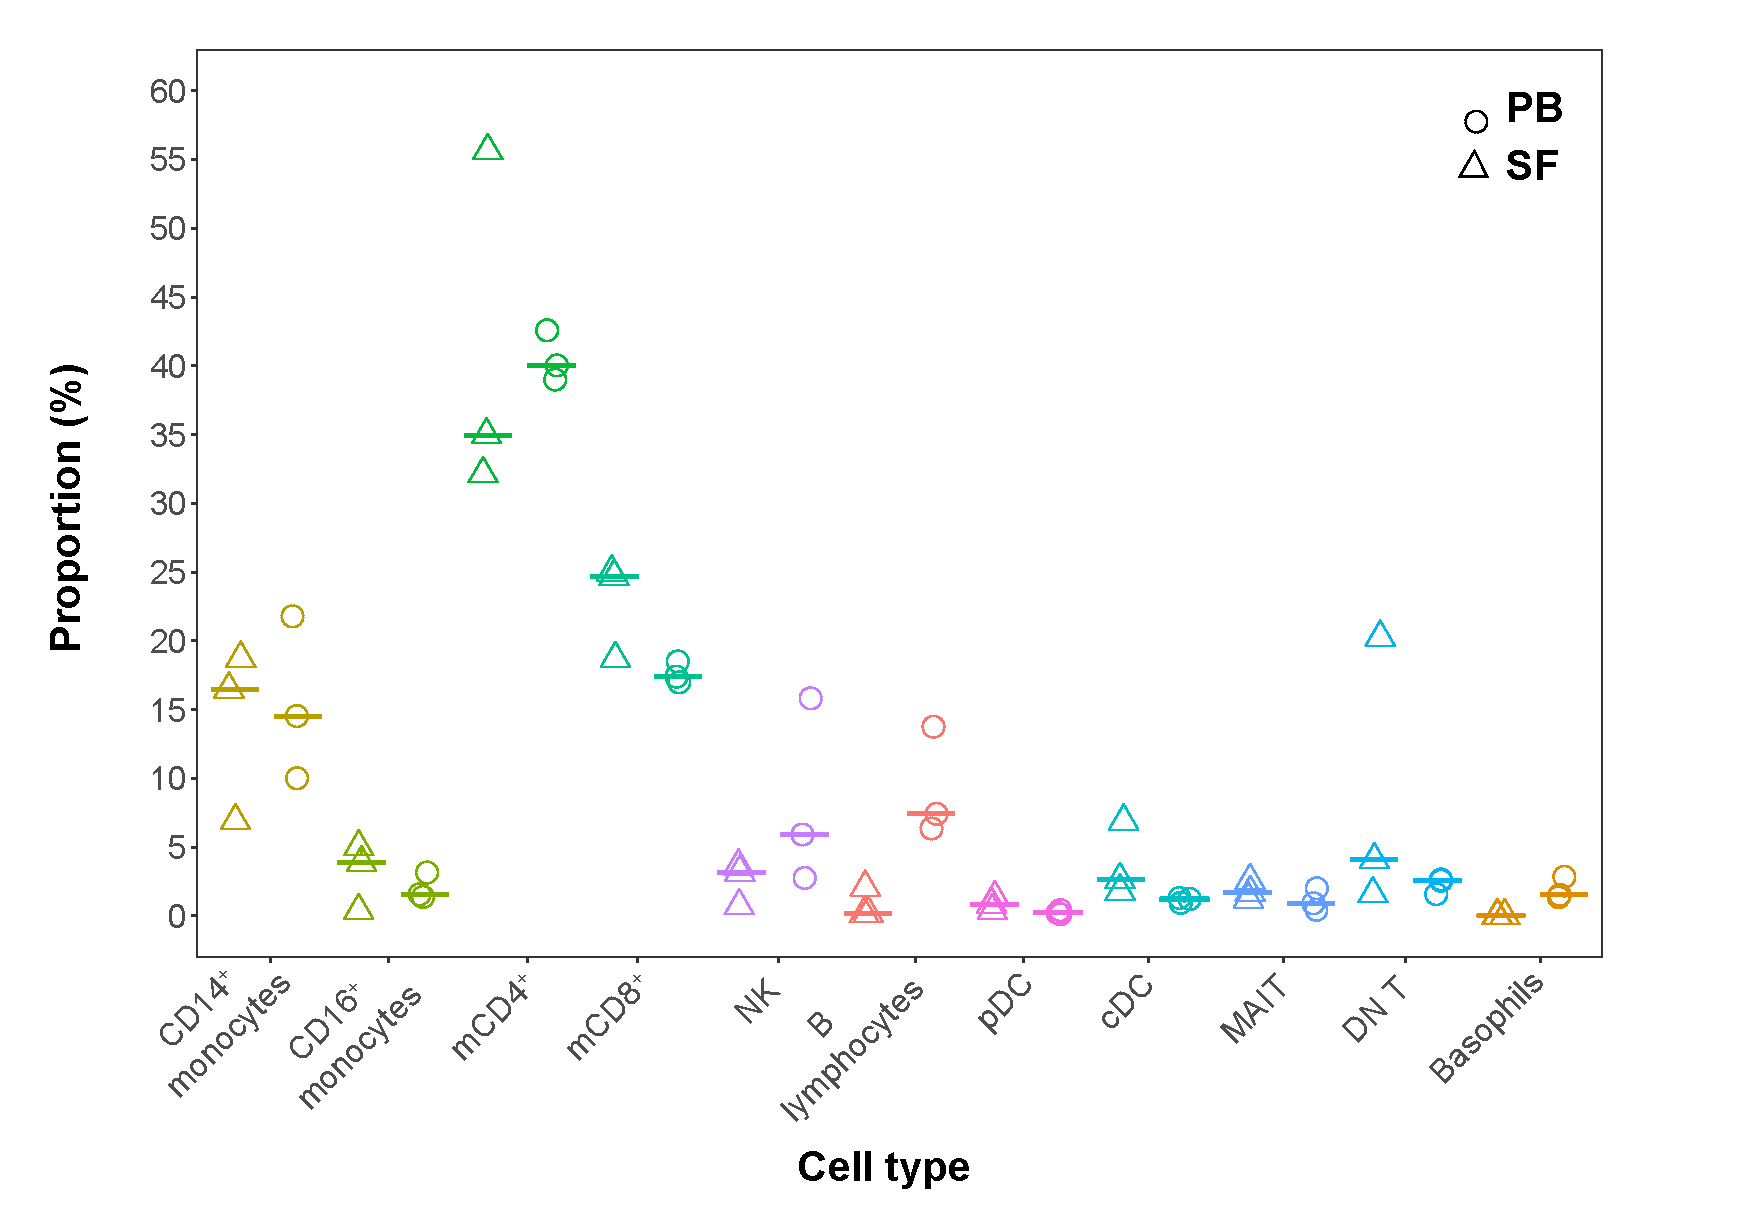
\includegraphics[width=0.7\textwidth]{./Results3/pdfs/PSA_ATAC_cohort_cell_type_composition_boxplots}
\caption[Comparative percentages of PB and SF immune cellular composition from the PsA cohort.]{\textbf{Comparative percentages of PB and SF immune cellular composition from the PsA cohort.} Percentages of each of the twelve cell types identified by mass cytometry are shown by individual and tissue for PsA1718, PsA1719 and PsA1607. Horizontal line represents the median percentage for a particular cell type in the appropriate tissue (SF or PB). Each of the cell types is displayed in a different colour. Central DC=cDC, mucosal-associated invariant T=MAIT, DN=double negative.)}
\label{figure:PsA_cell_composition}
\end{figure}



\subsection{Differential chromatin accessibility analysis in immune cells reveals differences between SF and PB}

\subsubsection{Quality control of Fast-ATAC data}
Twenty four Fast-ATAC PsA samples from four different cell types and two tissues (PB and SF) were sequenced and processes using the in-house pipeline as previously detailed in Chapter \ref{ch:Mat}. After filtering for low quality mapping, duplicates and MT reads, the median of total number of reads ranged between 46.6 and 70.2 millions (Figure \ref{figure:PsA_FAST_ATAC_QC} a). Overall, MT and duplicated reads accounted for a median of 40 to 62.2\% from the total number of unfiltered reads depending on cell type (Figure \ref{figure:PsA_FAST_ATAC_QC} b), contributing to the loss of reads in Fast-ATAC as previously detailed in Chapter \ref{ch:Results1}. %The final number of reads remaining after filtering was inversely related to the percentage of MT and duplicated reads identified. For example, mCD14$^+$ and mCD8$^+$ presented the lowest median of total number of reads after filtering concomitantly with the greatest percentage of combined MT and duplicated reads. 
%As previously mentioned, the MT DNA in ATAC-seq is one of the main sources of read loss, which is more accessible to the Tn5 transposase due to the absence of nucleosomes. Although the FAST-ATAC protocol represented an improvement, the percentage of MT reads across amongst all the samples ranged between 2.1 and 25.4\%. Similarly, despite initial optimisation of the number of PCR cycles used in the library amplification, the duplicated reads still represented between 22.9 to 55\% of the total number sequenced reads.

Regarding sample quality, TSS enrichment analysis showed differences in the levels of background noise across cell types and highlighted the variability of Fast-ATAC performance (Figure \ref{figure:PsA_FAST_ATAC_QC} c). A general trend towards greater TSS enrichment in PB samples compared to SF was observed. mCD4$^+$ and mCD8$^+$ presented the best signal-to-noise ratios, with median of 19.1 and 23.1 fold enrichment, respectively. In contrast, NK was the cell type with the lowest TSS enrichment values. Particularly, the fold enrichment for PsA1719 and PsA1607 in NK were close to the 6 fold enrichment considered by ENCODE as acceptable. If a larger cohort size was available these two samples would be removed from the differential analysis to prevent excessive noise to reduce the power of the differential analysis. 

 
\bigskip
\begin{figure}[H]
\centering
\begin{subfigure}[b]{0.48\textwidth}
\centering 
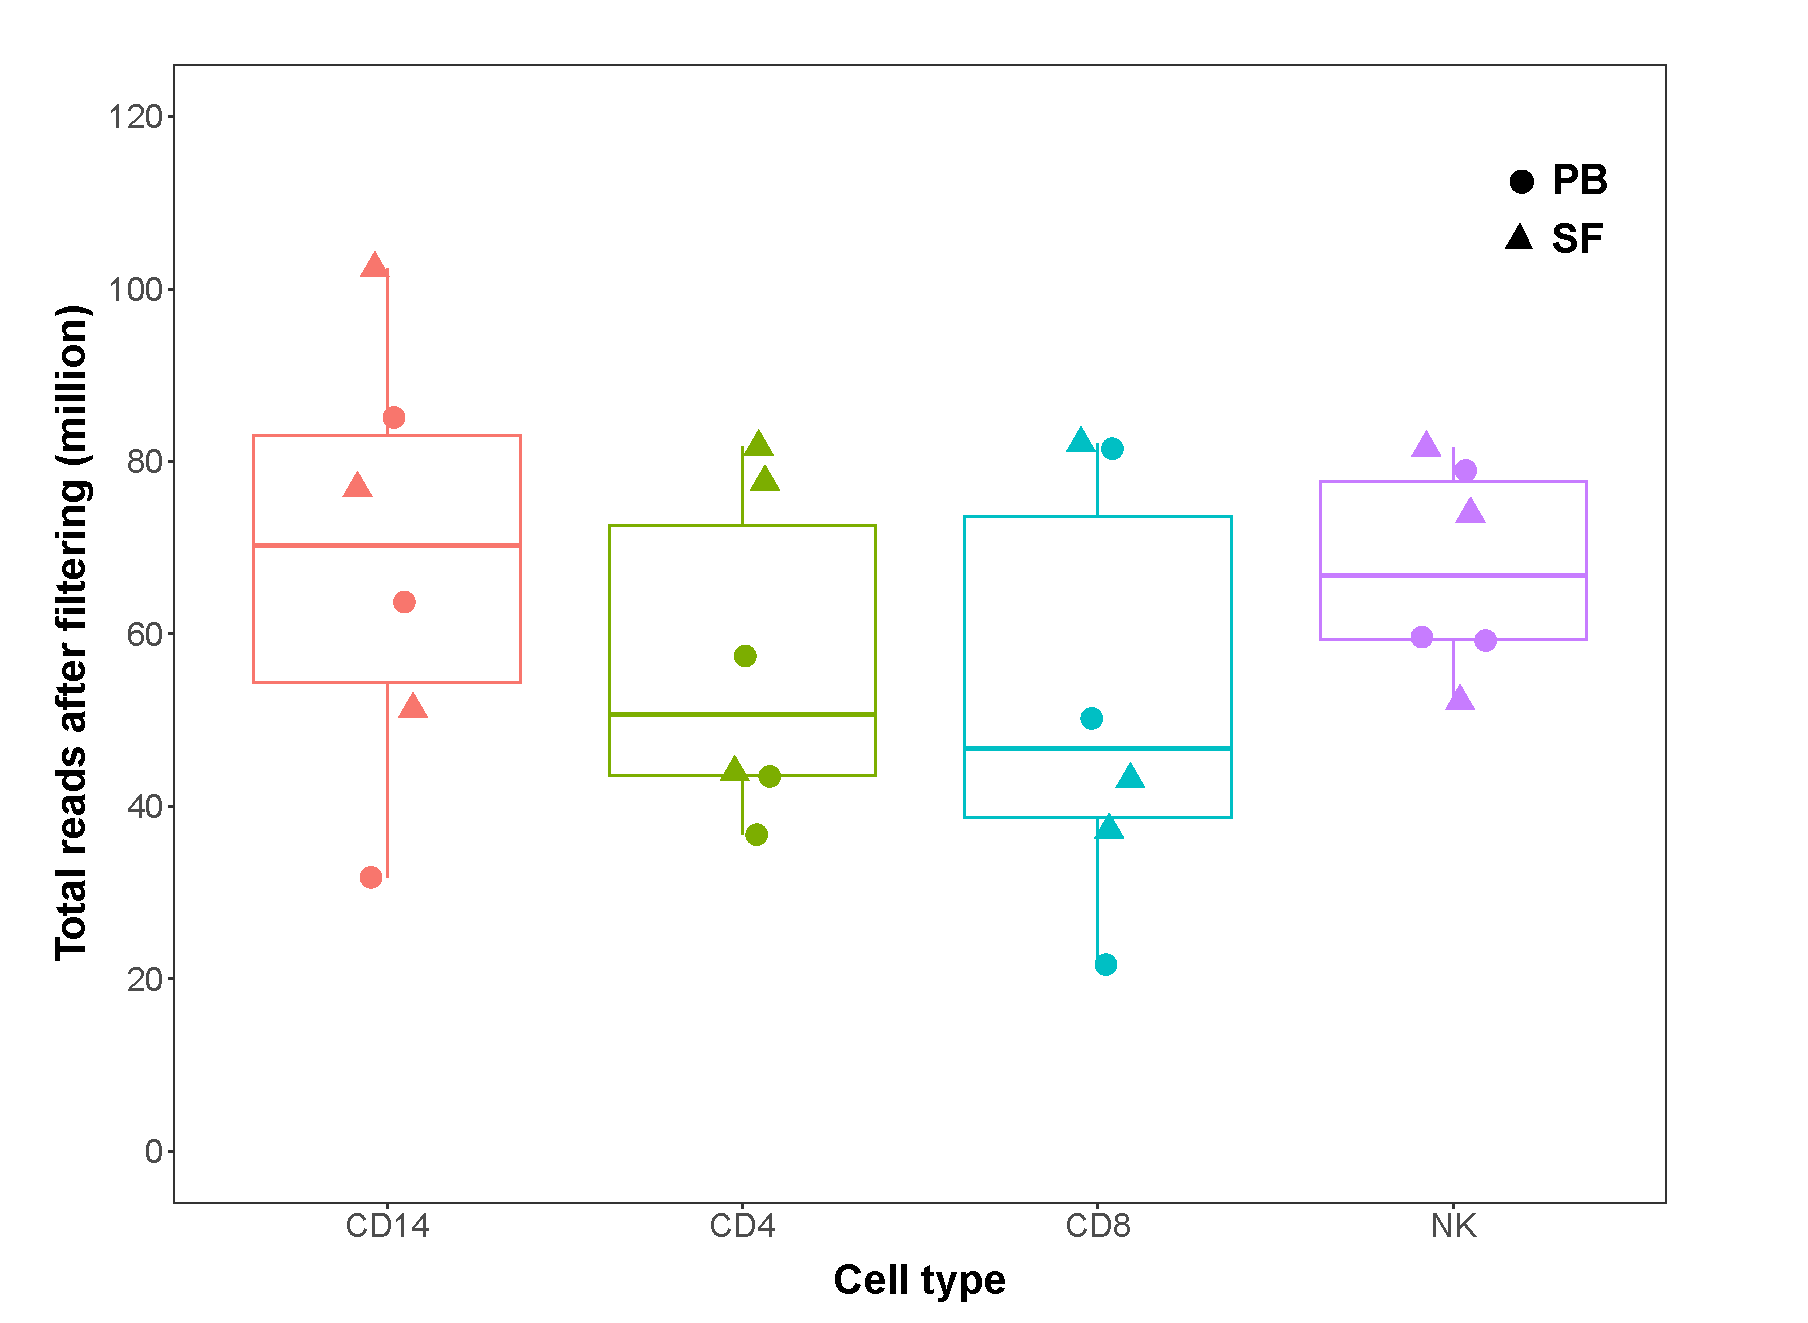
\includegraphics[width=\textwidth]{./Results3/pdfs/ATAC_PSA_total_filtered_reads_boxplot}
\caption{}
\end{subfigure}
~
\begin{subfigure}[b]{0.48\textwidth}
\centering 
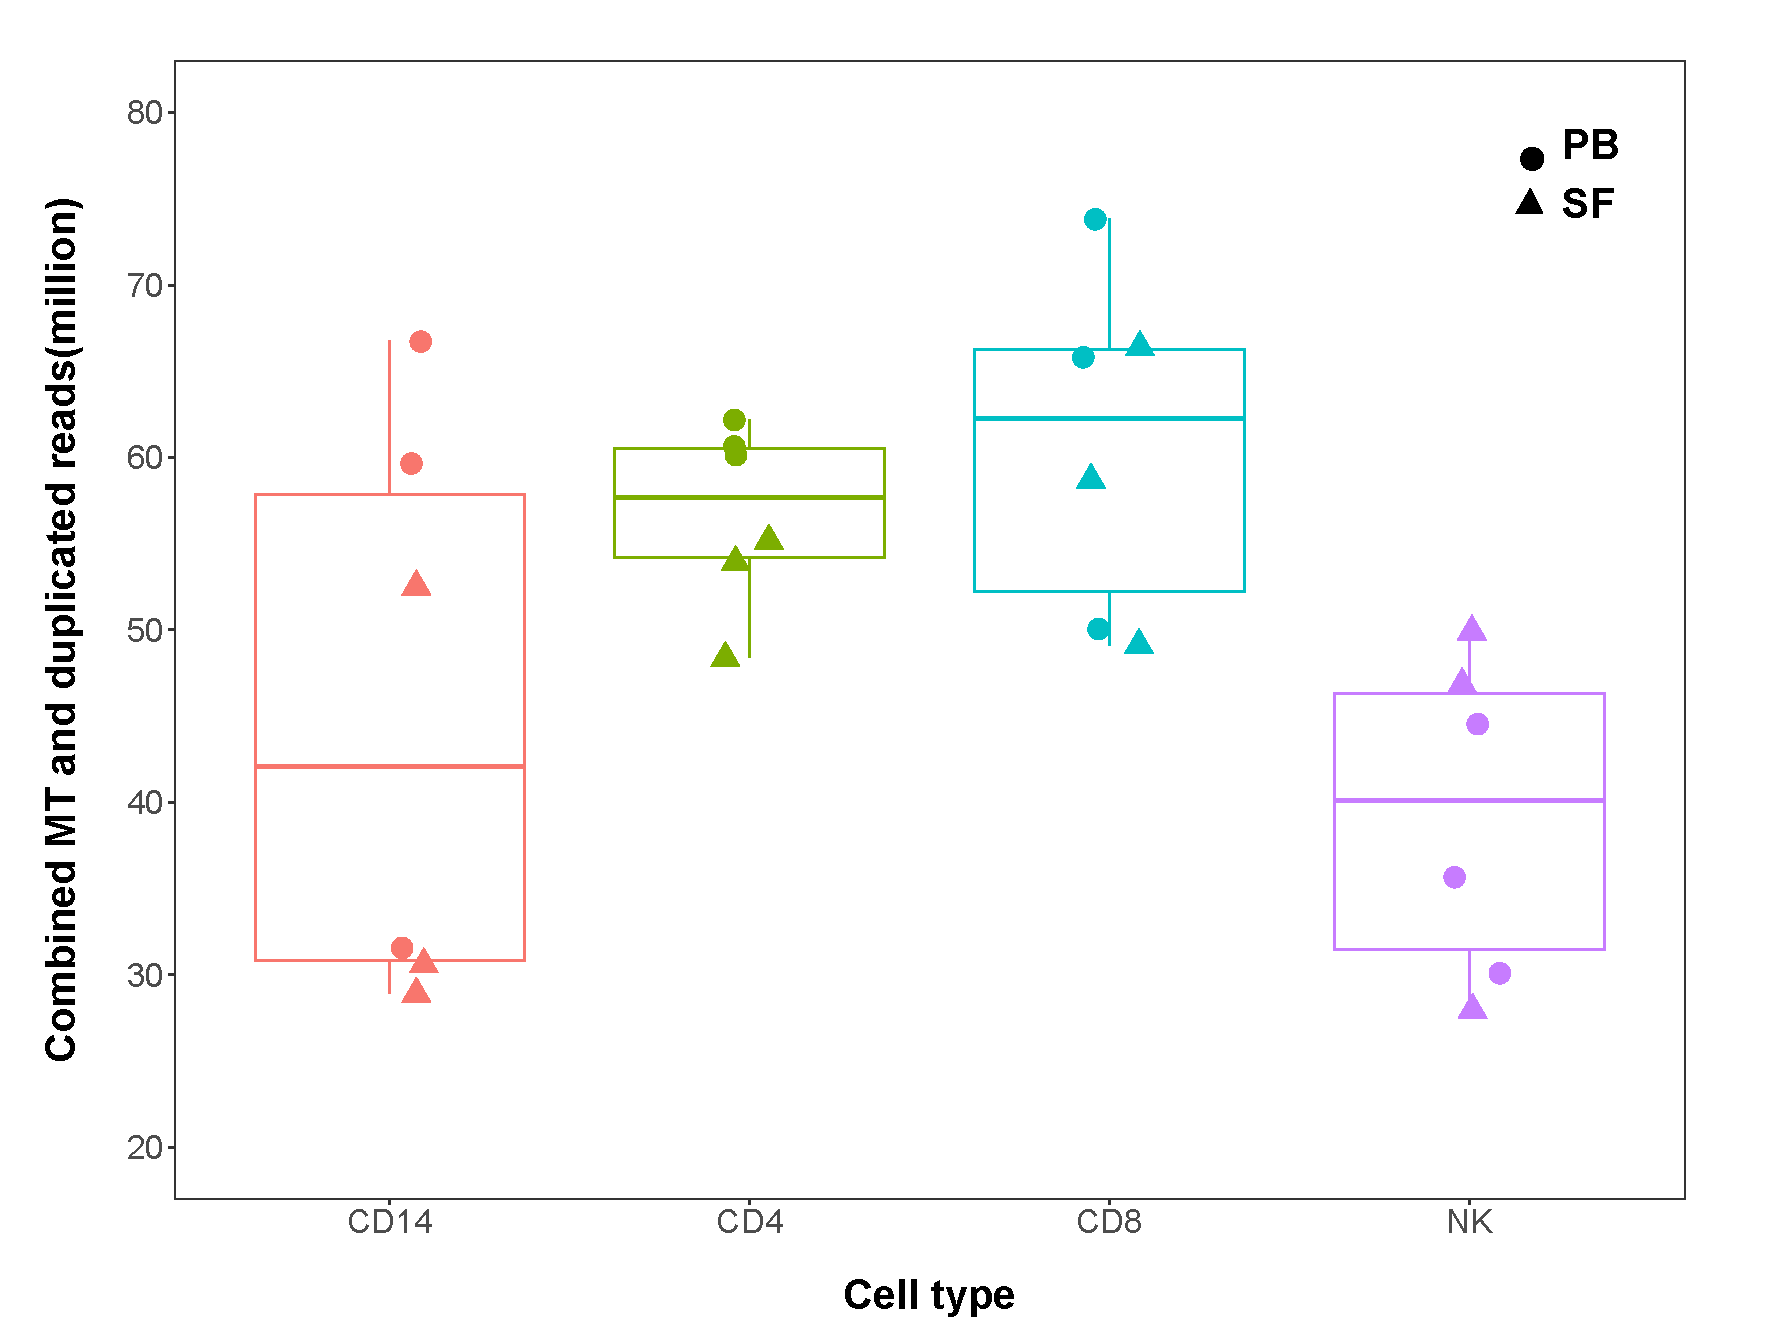
\includegraphics[width=\textwidth]{./Results3/pdfs/ATAC_PSA_pcnt_dups_and_MT_reads_boxplot}
\caption{}
\end{subfigure}
~
\begin{subfigure}[b]{0.48\textwidth} 
%the [b] prevents offset in subcaptions
\centering
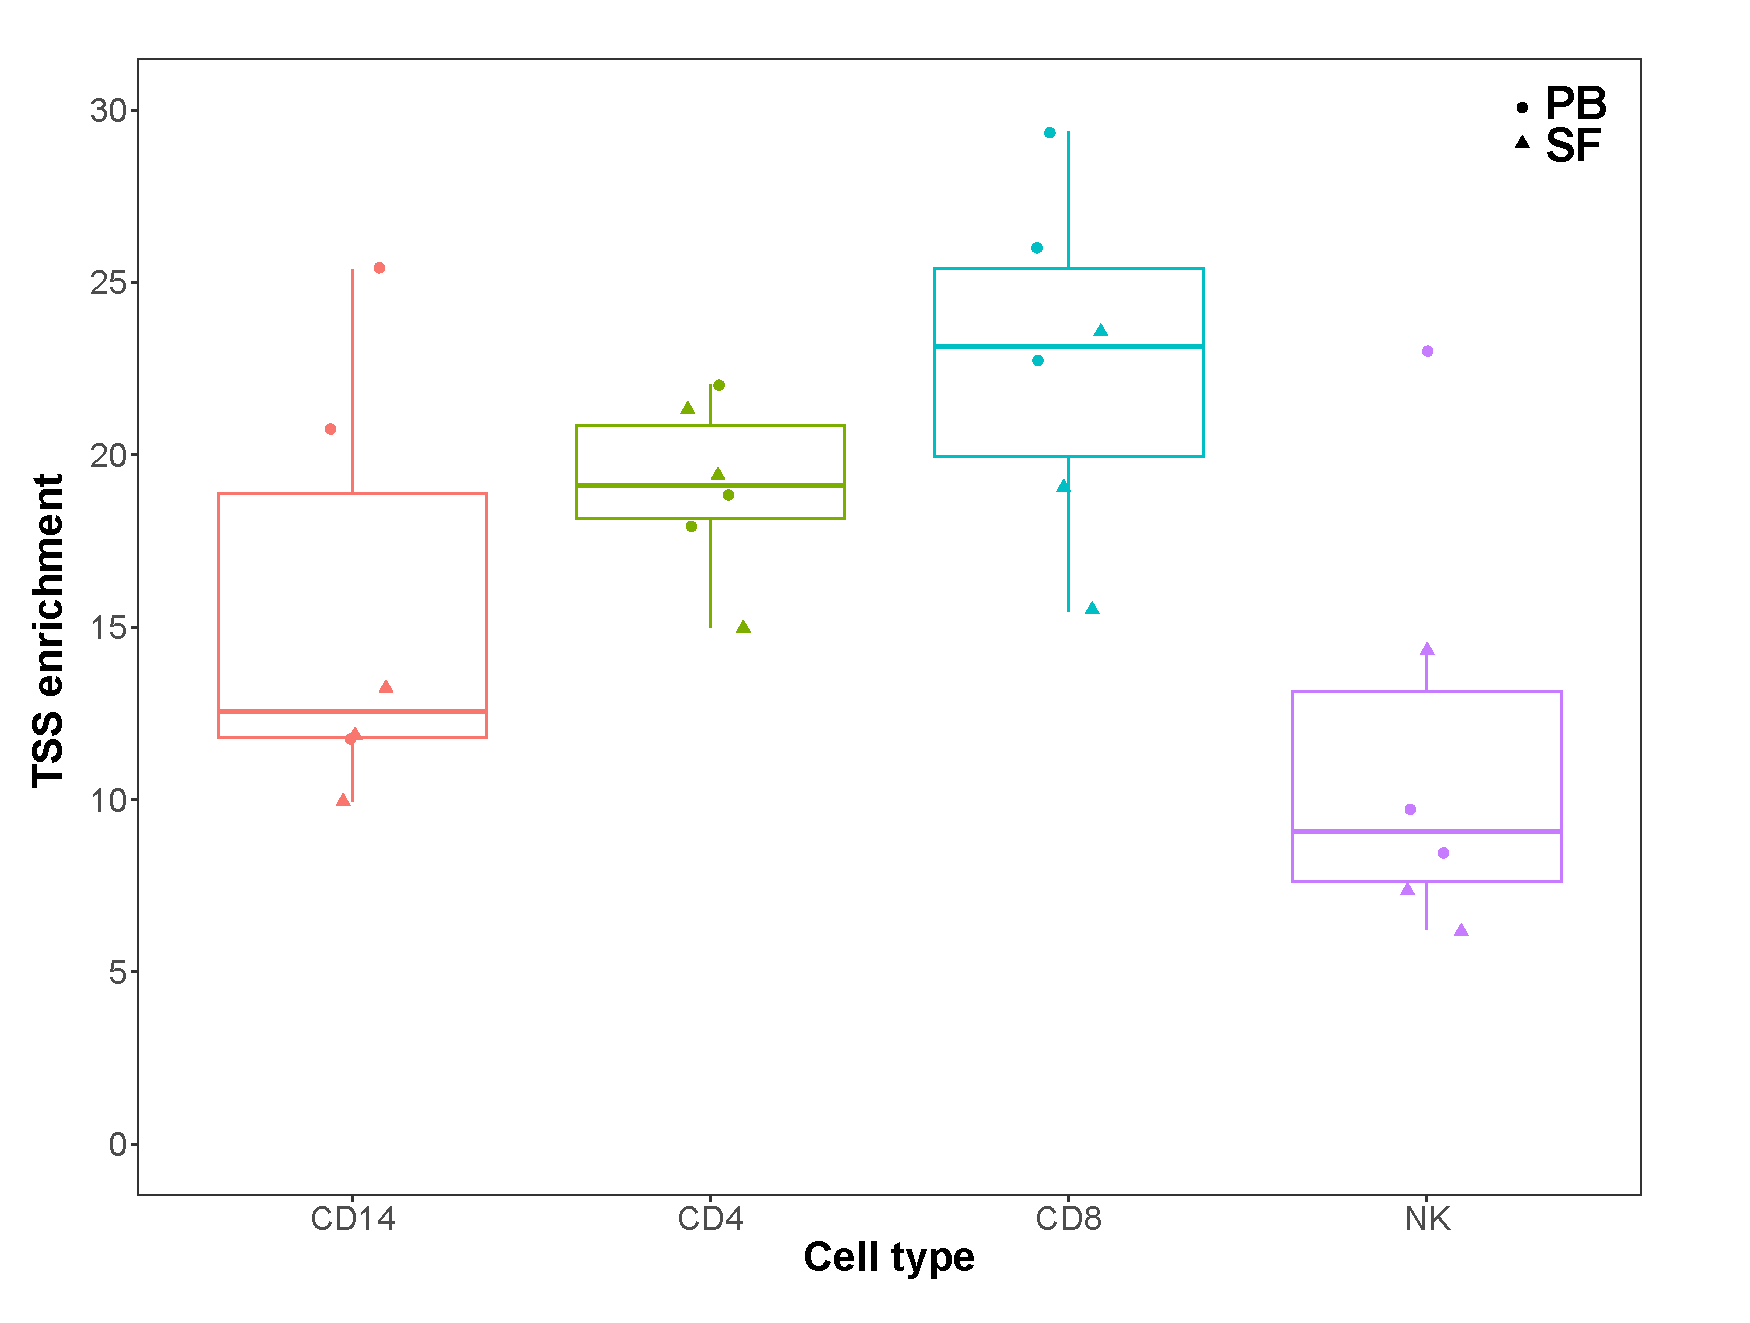
\includegraphics[width=\textwidth]{./Results3/pdfs/ATAC_PSA_all_TSS_max_per_cell_type}%
\caption{}
\end{subfigure}
\begin{subfigure}[b]{0.48\textwidth} 
%the [b] prevents offset in subcaptions
\centering
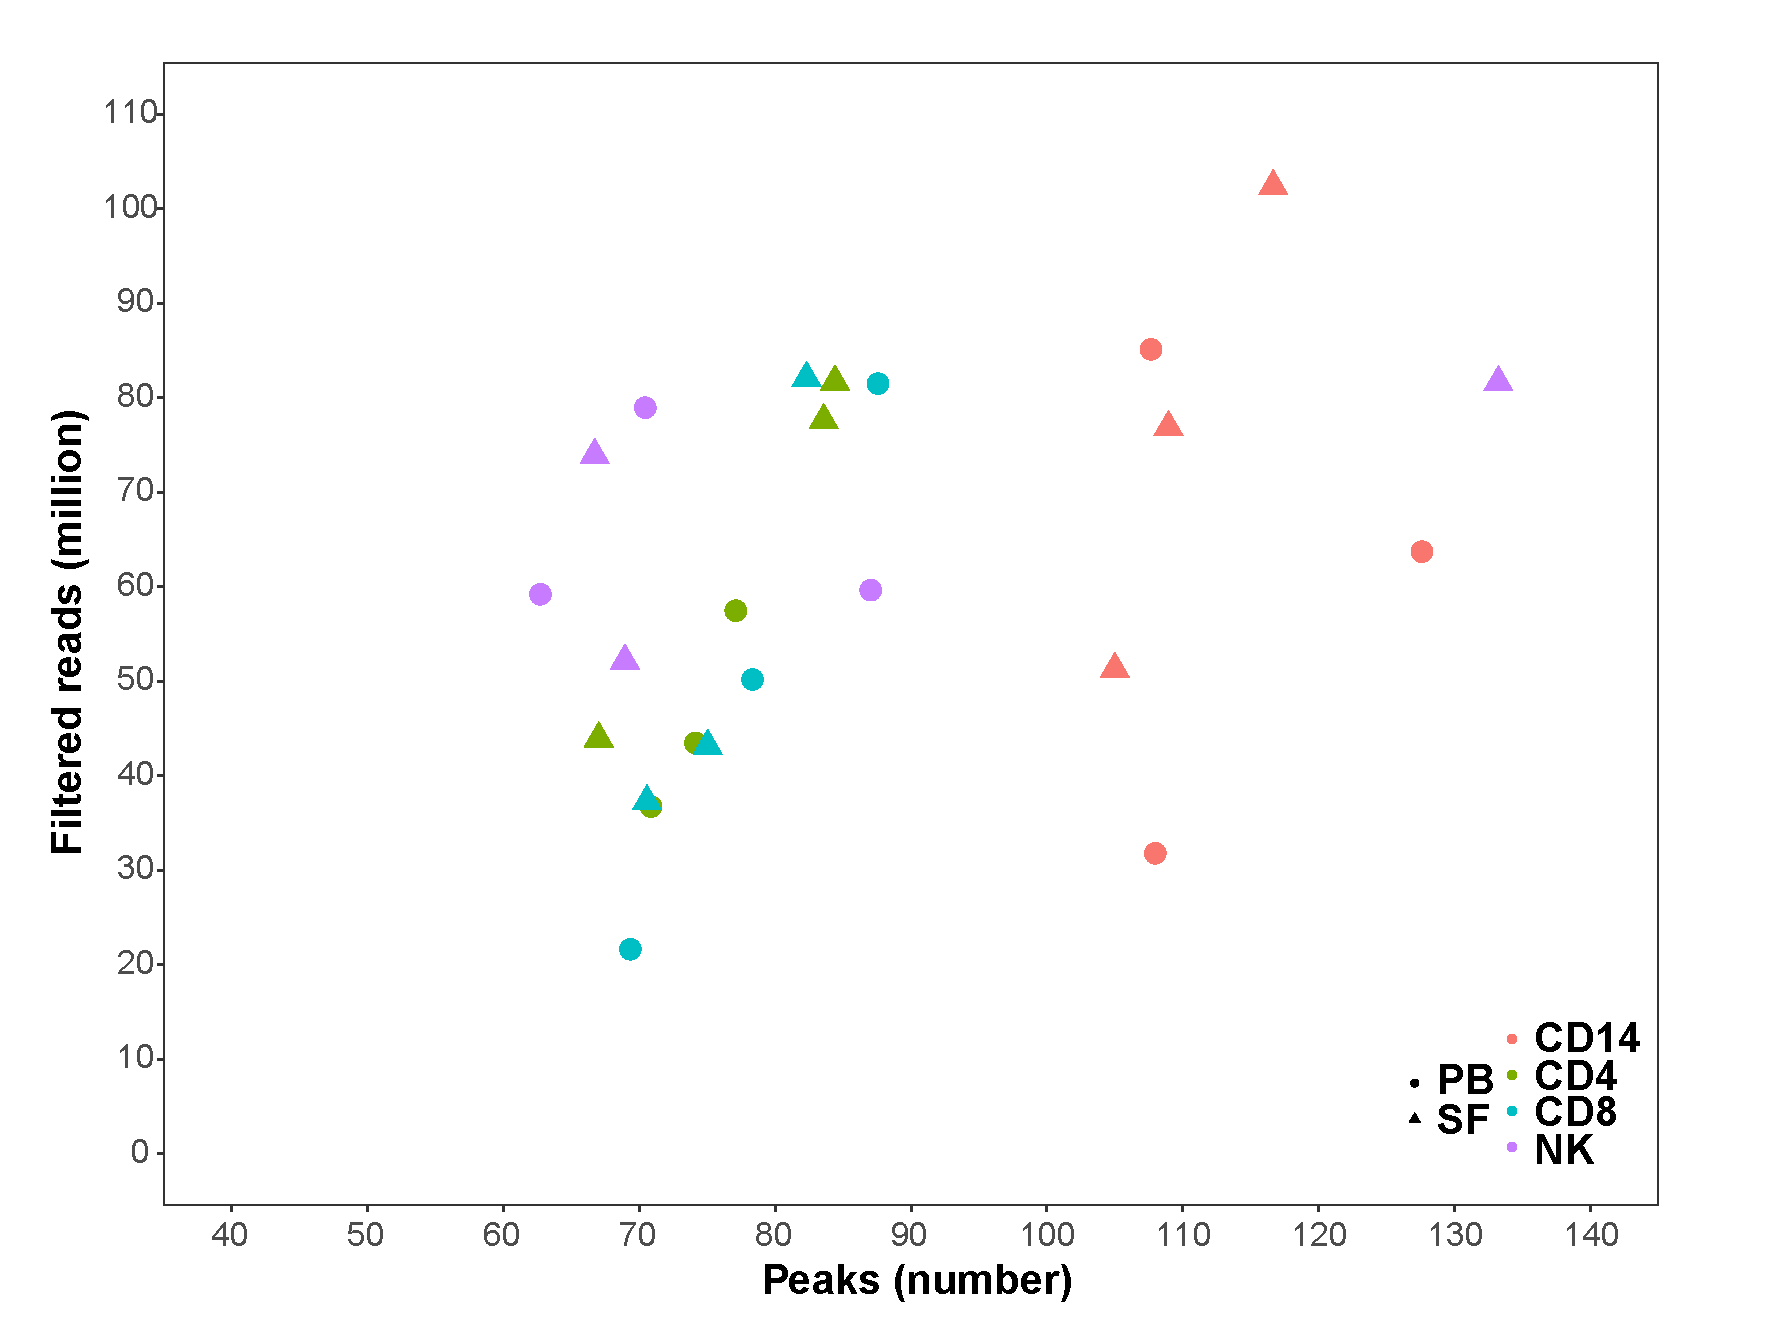
\includegraphics[width=\textwidth]{./Results3/pdfs/ATAC_PSA_all_peaks_vs_num_reads}%
\caption{}
\end{subfigure}
\caption[Quality control assessment of the ATAC-seq data generated in four immune cell types isolated from PB and SF of PsA patients samples.]{\textbf{Quality control assessment of the ATAC-seq data generated in four immune cell types isolated from PB and SF of PsA patients samples.} Significant differentially accessible regions for FDR$<$0.01 and absolute FC$>$1.5.}
\label{figure:PsA_FAST_ATAC_QC}
\end{figure}

When identifying open chromatin regions by peak calling followed by pval filtering based on IDR analysis, the number of accessible regions per sample ranged approximately between 24x10$^3$ and 97x10$^3$ (Figure \ref{figure:PsA_FAST_ATAC_QC} d). The total number of called peaks passing filtering varied across cell types and was influenced by the quality sample, as previously demonstrated in Chapter \ref{ref:Results1}. Overall, appropriate number of peaks were called in all the samples and no concerning outliers were identified.
%For example, CD14$^+$ was the cell type with greatest number of called peaks (108.4$x10^3$) as well as the greater median of reads remaining after filtering when compared to the other three cell types (Figure \ref{figure:PsA_FAST_ATAC_QC} a). 
%For example, the two NK samples with the greatest TSS enrichment (PSA1718 SF and PB) showed larger number of called peaks when compared to the other NK samples with similar number of reads but lower quality measured by TSS enrichment. This observation was consistent with the correlation between sample quality and the number of identified accessible chromatin regions previously demonstrated in Chapter \ref{ch:Results1}. 


\subsubsection{Accessible chromatin reflects cell type specificity and functional relevance}
A consensus master list of accessible chromatin regions identified across all the samples and cell types (ML\_ALL) was built, as previously explained in Chapter \ref{ch:Mat} and Chapter \ref{ch:Results1}. PCA analysis based on the normalised counts for each region of the ML\_ALL showed that most of the variability (PC1 65.6\% of the variability) in the chromatin landscape correlated with cell type, leading to sample separation in four cluster (Figure \ref{figure:PsA_FAST_ATAC_PCA}). The myeloid (CD14$^+$ monocytes) and lymphoid (mCD4$^+$ and mCD8$^+$) clusters appeared as the most different between them based on the Fast-ATAC profile. Conversely,the mCD4$^+$ and mCD8$^+$ clusters were the most similar between them, altogether supporting the ability of Fast-ATAC to capture cell type chromatin accessibility features. In addition to this, modest separation between SF and PB samples was also found in the mCD4$^+$, mCD8$^+$ and NK clusters (Figure \ref{figure:PsA_FAST_ATAC_PCA}).

\begin{figure}[H]
\centering
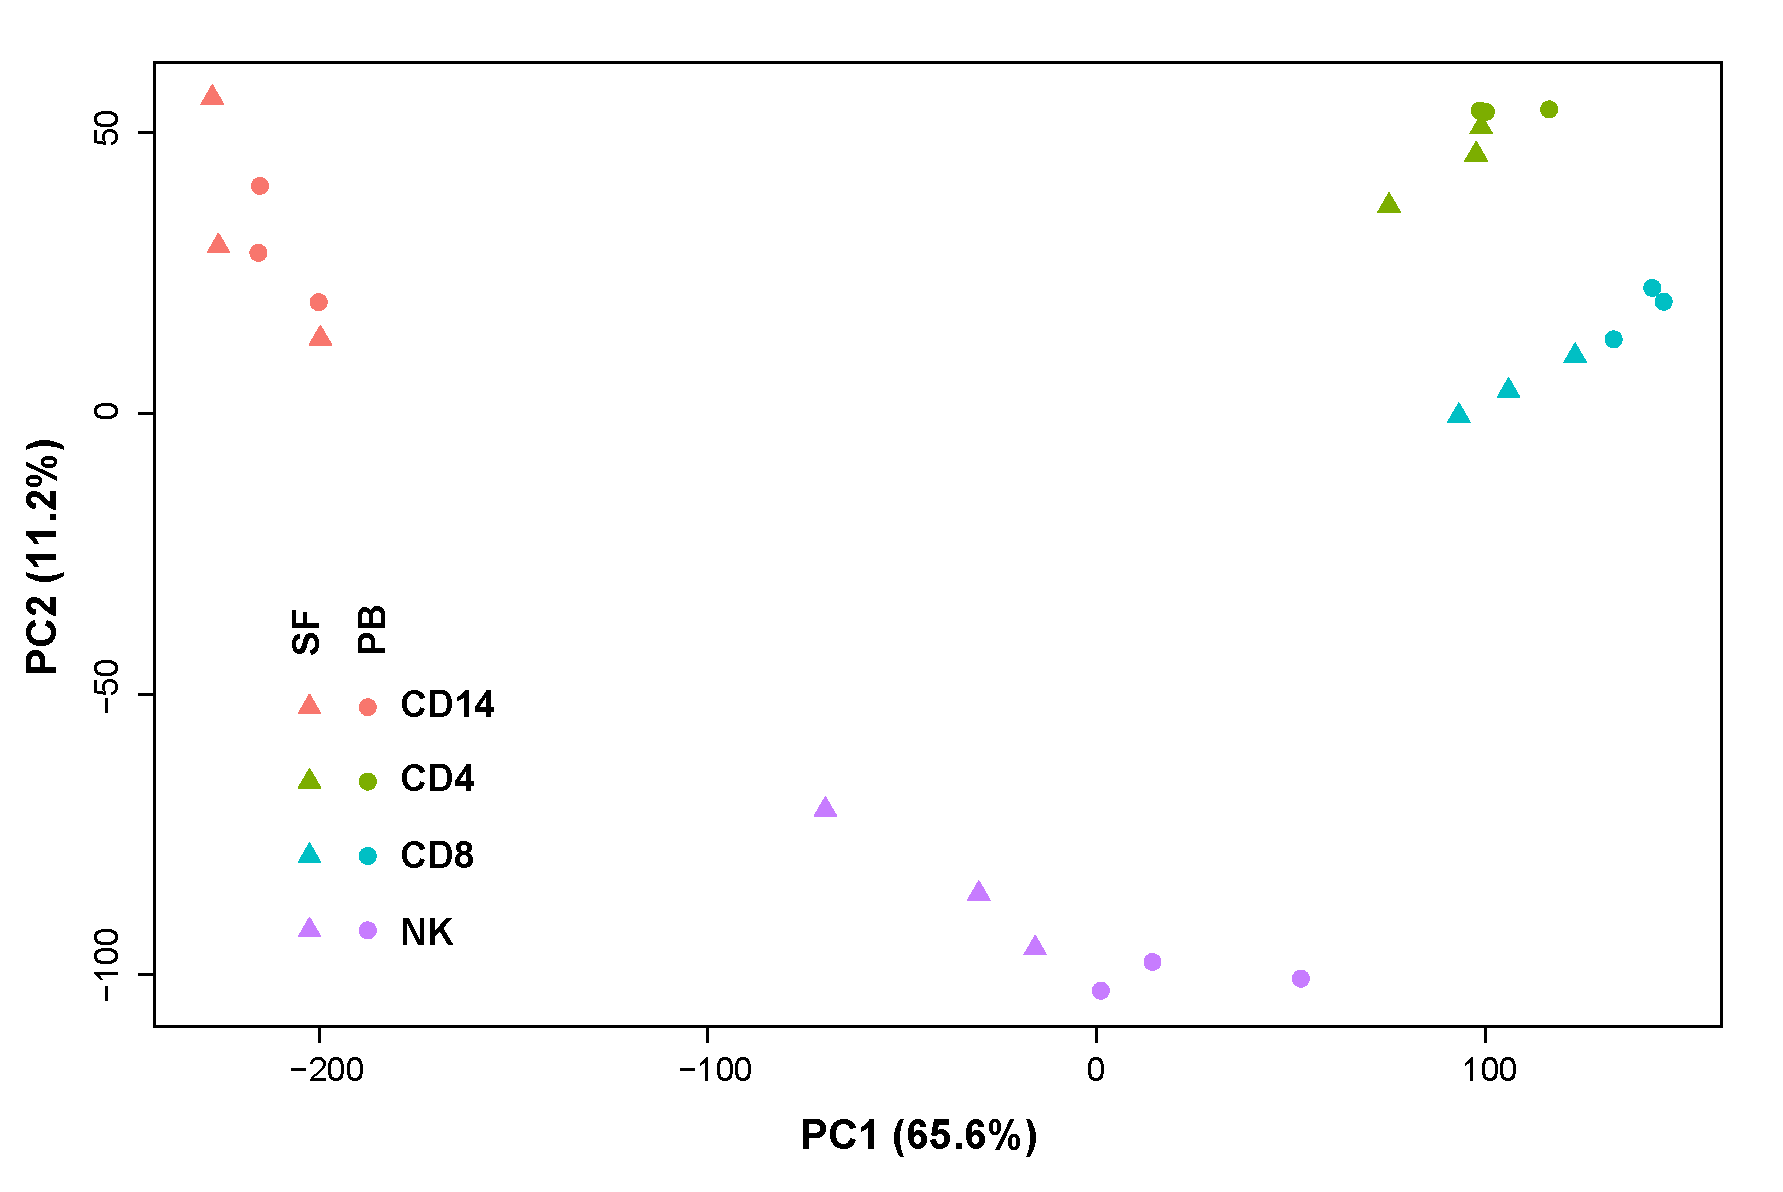
\includegraphics[width=0.7\textwidth]{./Results3/pdfs/ATAC_PSA_all_DESEq2_PCA}
\caption[Combined PCA analysis of all four cell types isolated from blood and SF.]{\textbf{Combined PCA analysis of all four cell types isolated from blood and SF.}x}
\label{figure:PsA_FAST_ATAC_PCA}
\end{figure}

The ability to capture putative regulatory regions within the identified accessible chromatin regions was also explored. Enrichment analysis of different eQTL publicly available datasets for the regions contained in the MASTER\_ALL list was performed. Amongst the GTEx eQTL data, the largest (z-score) and most significant (-log$_10$FDR) enrichment was found for the venous blood data set (red dot), consistent with the cell types included in the study (Figure \ref{figure:PsA_FAST_ATAC_eQTL_enrichment} a). In terms of publicly available eQTLs studies in immune cells, the strongest enrichment for the MASTER\_ALL regions were found for CD14$^+$ monocytes (importantly unstimulated, LPS 2h and IFN-$\gamma$ 24h) followed by mCD8$^+$ T cells (Figure \ref{figure:PsA_FAST_ATAC_eQTL_enrichment} b).

\bigskip
\begin{figure}[H]
\centering
\begin{subfigure}[b]{0.5\textwidth}
\centering 
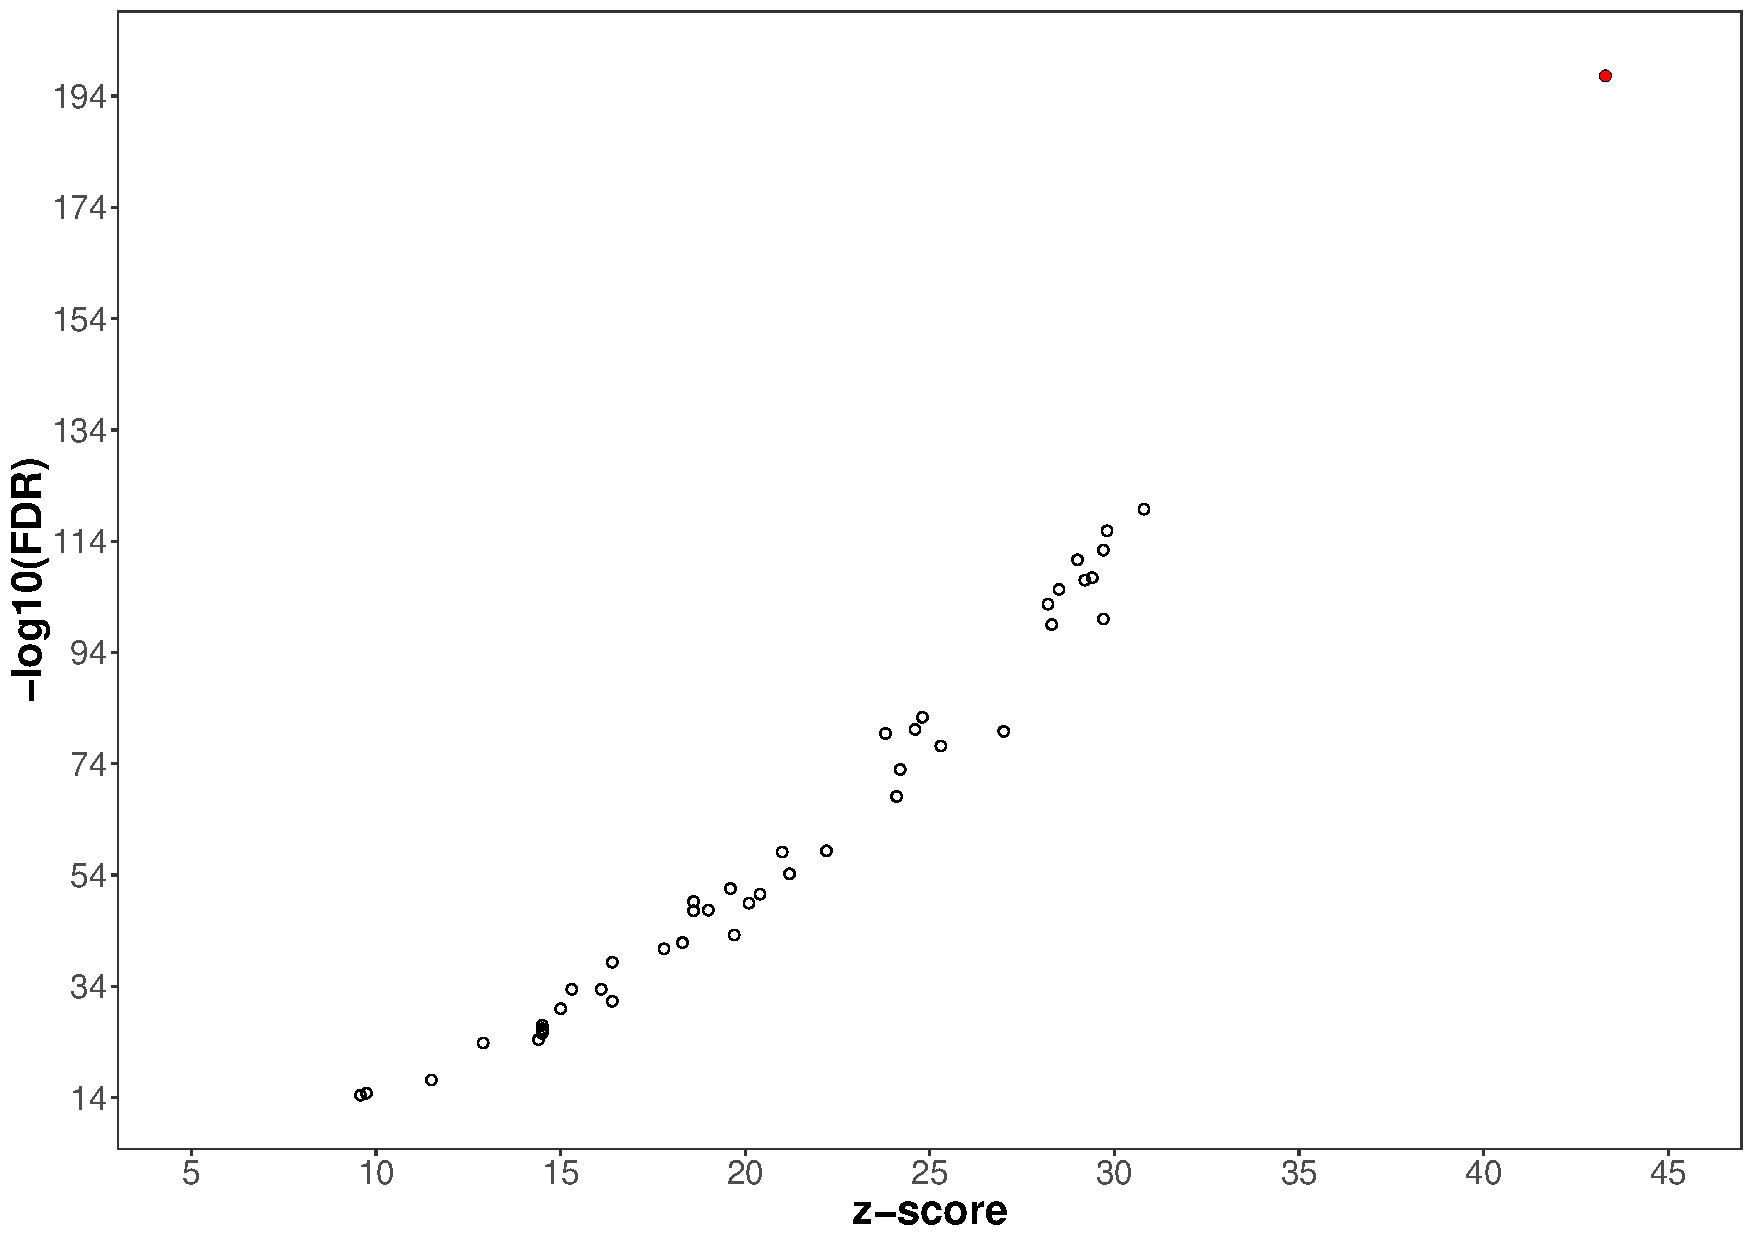
\includegraphics[width=\textwidth]{./Results3/pdfs/ATAC_PSA_all_GTeX_eQTL_enrichment_dotplot}
\caption{}
\end{subfigure}
\begin{subfigure}[b]{0.5\textwidth} 
%the [b] prevents offset in subcaptions
\centering
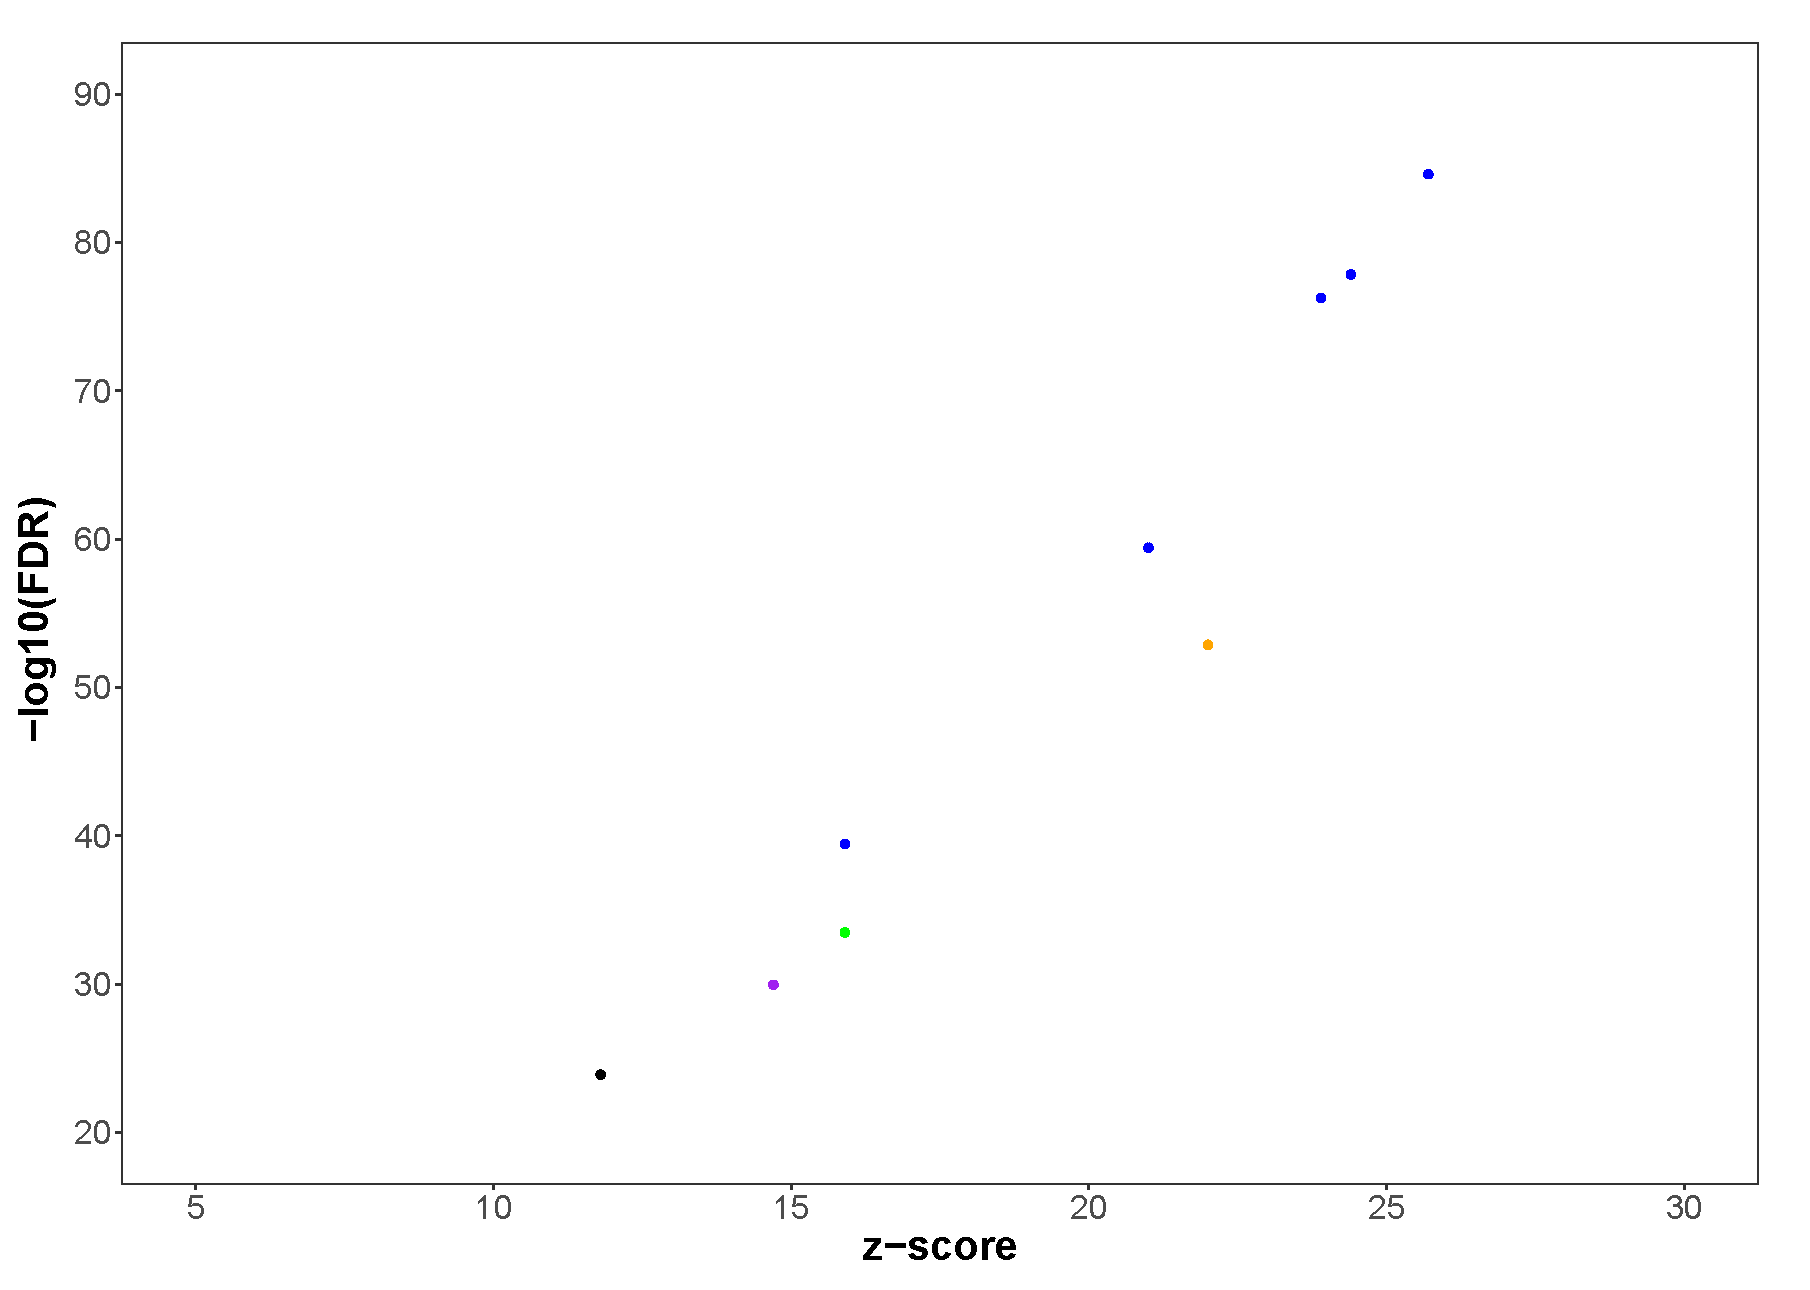
\includegraphics[width=\textwidth]{./Results3/pdfs/ATAC_PSA_all_Jknight_eQTL_enrichment_dotplot}
\caption{}
\end{subfigure}
\caption[Enrichment of eQTLs publicly available data in the combined cell type and tissue chromatin accessibility master list for the PsA cohort.]{\textbf{Enrichment of eQTLs publicly available data in the combined cell type and tissue chromatin accessibility master list for the PsA cohort.} The dot plots showed the z-score values of the enrichment analysis in the x-axis and the significance (-log$_10$FDR) in the y-axis for a) GTEx eQTL datasets and b) non-GTEx immune-related cell types including CD14$^+$ monocytes (unstimulated, 2 or 24h LPS stimulated and 24h IFN$\gamma$ stimulated) in blue, B cells in black, total CD4$^+$ in green, total CD8$^+$ in orange and neutrophils in purple.}
\label{figure:PsA_FAST_ATAC_eQTL_enrichment}
\end{figure}





\subsubsection{Characterisation of the differential accessible chromatin regions}
A consensus master list of chromatin accessible regions was built for each of the four cell types of interest (ML\_CD14, ML\_CD4, ML\_CD8 and ML\_NK). Differential chromatin accessibility analysis between SF and PB was performed on the normalised counts retrieved for each of the cell type master lists using DESeq2 and a paired design (Table \ref{tab:PSA_DOCs_results}). A 80\% cut-off for background noise was used to filter the count matrix, as previously explained in Chapter \ref{Results3}. %Only differentially accessible regions (DARs) identified with DESeq2 and also shared with quantile normalisation limma voom analysis where considered downstream. 
The CD14$^+$ monocytes and NK were the two cell types presenting the greatest total number (5,285 and 2,314, respectively) and proportion of DARs (23.3 and 8.9\%, respectively). For each cell type, DARs were divided in DARs more open in SF compared to PB (SF open DARs) and DARs less open in SF compared to PB (PB open DARs). In CD14$^+$ monocytes the number of SF open DARS were notably larger than the number of PB open DARs (3,779 and 1,506DARs, respectively) (Table \ref{tab:PSA_DOCs_results}). Conversely, the number of SF and PB open DARs were similar for the other three cell types.


\begin{table}[htbp]
%\setlength{\tabcolsep}{20pt} only to stretch the columns if you want
%\renewcommand{\arraystretch}{1.5}
\centering
\begin{tabular}{@{}c c c c c}
\toprule
\textbf{Cell type}  & \textbf{Total DARs} &  \textbf{Proportion}  & \textbf{SF open} & \textbf{PB open} \\
                    &                     &  \textbf{DARs (\%)}  & \textbf{DARs} & \textbf{DARs} \\
\midrule
\midrule
CD14$^+$ & 5,285 & 23.3 & 3,779 & 1,506 \\
CD4$^+$  & 1,329 & 4.3 & 621 & 708 \\
CD8$^+$  & 1,570 & 4.5 & 807 & 763 \\
NK       & 2,314 & 8.9 & 1,223 & 1,091 \\
\bottomrule
\end{tabular}
\medskip %gap
\caption[Summary results of the differential chromatin accessibility analysis between SF and PB in PsA samples.]{\textbf{Summary results of the differential chromatin accessibility analysis between SF and PB in PsA samples.}}
\label{tab:PSA_DOCs_results}
\end{table}

Permutation analysis was used to determine if the large number of DARs (particularly by comparison to limited finding in the psoriasis analysis) were more than would be expected by chance. None of the ten possible permutations demonstrated a greater number of DARs than the ones identified for the true groups, reinforcing the robustness of the differential analysis results (Figure \ref{figure:PsA_perm_analysis}).

  
Genomic annotation of the DARs identified in each the cell types revealed that 80\% or more of all regions with differential accessibility were located at intronic and intergenic regions (Figure \ref{figure:PsA_FAST_ATAC_DOCS_annotation} a). Universal promoter regions was the third most represented genomic feature, accounting for the annotation of approximately between 5 to 15\% of the DARs in each cell type. In addition to this, the chromatin states from the Roadmap Epigenomics maps were also used for annotation (Figure \ref{figure:PsA_FAST_ATAC_DOCS_annotation} b). For all four cell types,  between 44.96 and 72.11\% of the DARs were annotated as weak enhancers, which represented the most prominent category and the most significantly enriched (data not shown). This over-representation of enhancers was consistent with large percentage of introns and intergenic regions found for the genomic features annotation, as those are the preferred location for enhancer elements. Modest percentages of DARs were annotated as heterochromatin and repetitive regions but not significant enrichment for these two chromatin states was found for any of the four cell types (Figure \ref{figure:PsA_FAST_ATAC_DOCS_annotation} b).
%

\bigskip
\begin{figure}[H]
\centering
\begin{subfigure}[b]{0.5\textwidth}
\centering 
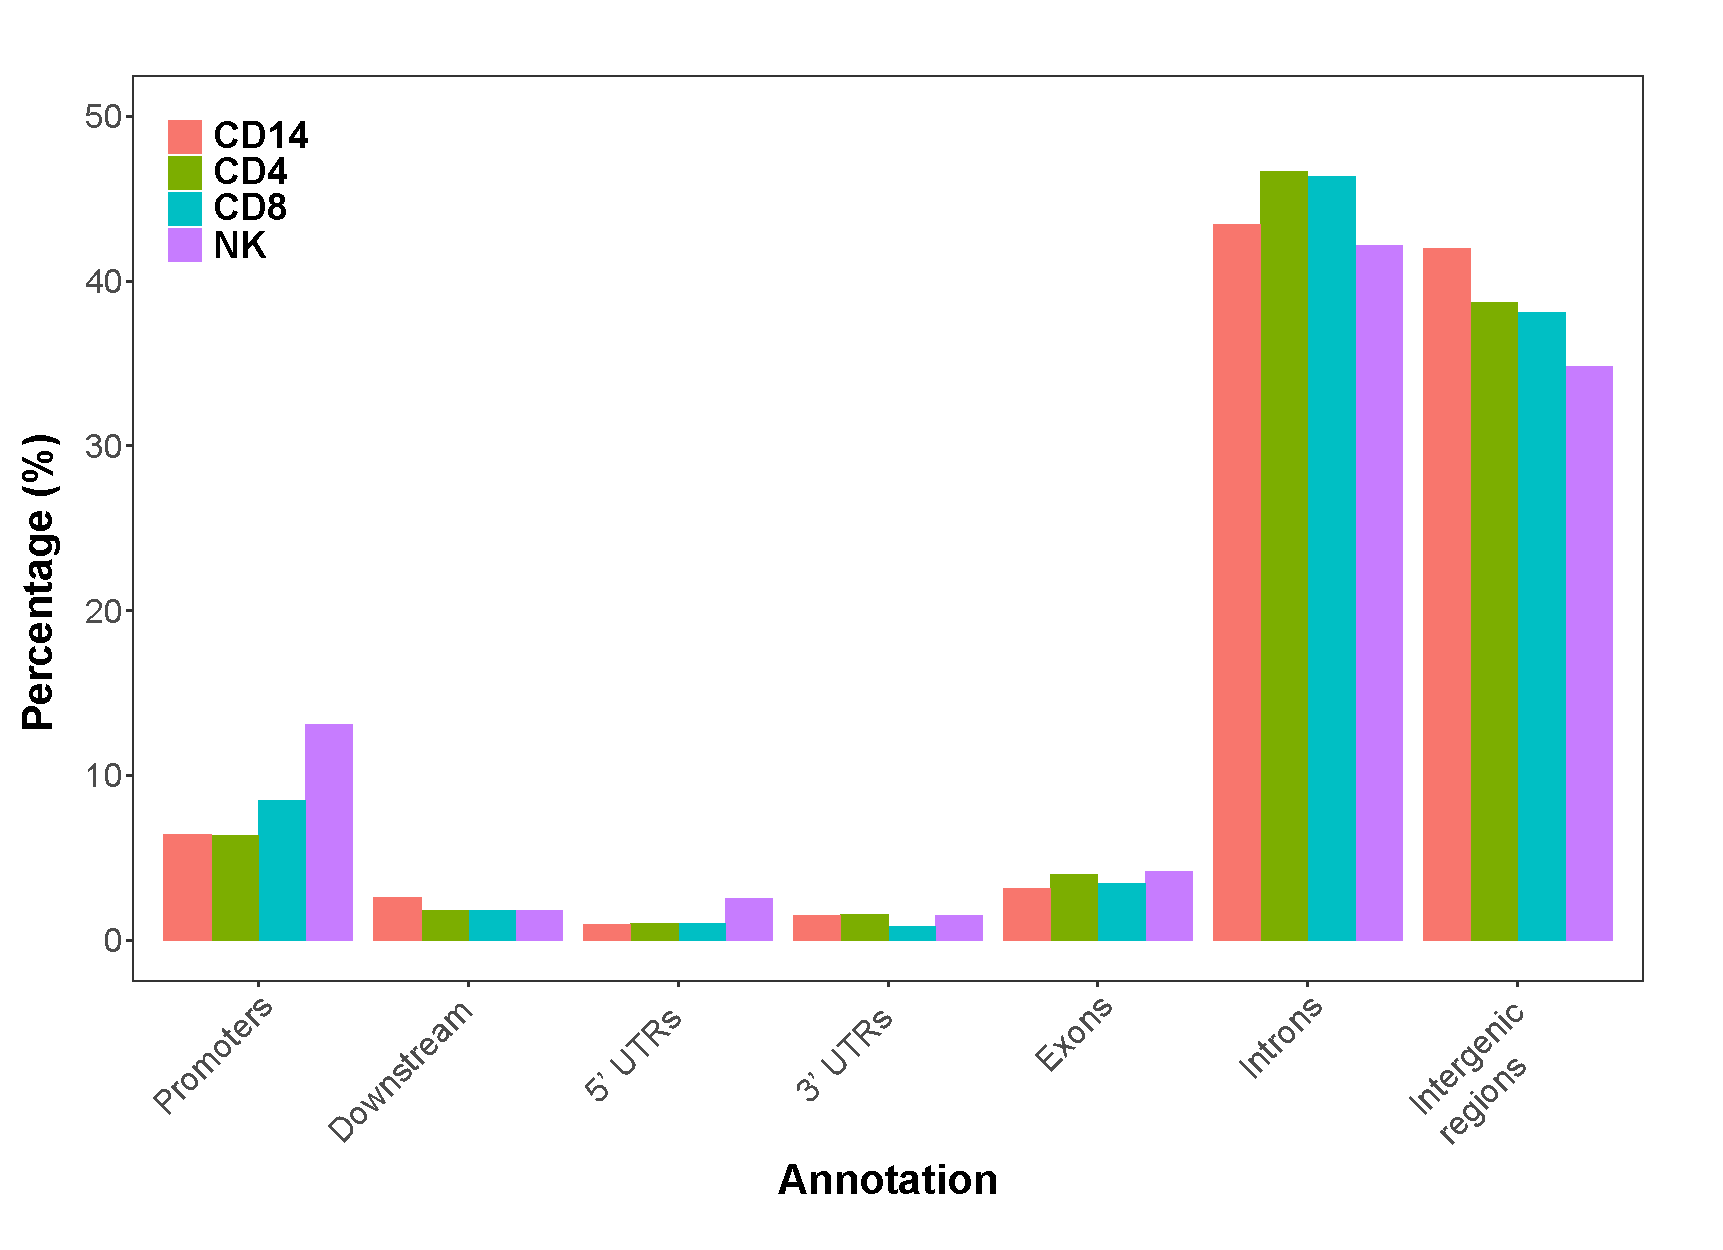
\includegraphics[width=\textwidth]{./Results3/pdfs/ATAC_PSA_DOCS_per_cell_type_general_annotation}
\caption{}
\end{subfigure}
~
\begin{subfigure}[b]{0.6\textwidth} 
%the [b] prevents offset in subcaptions
\centering
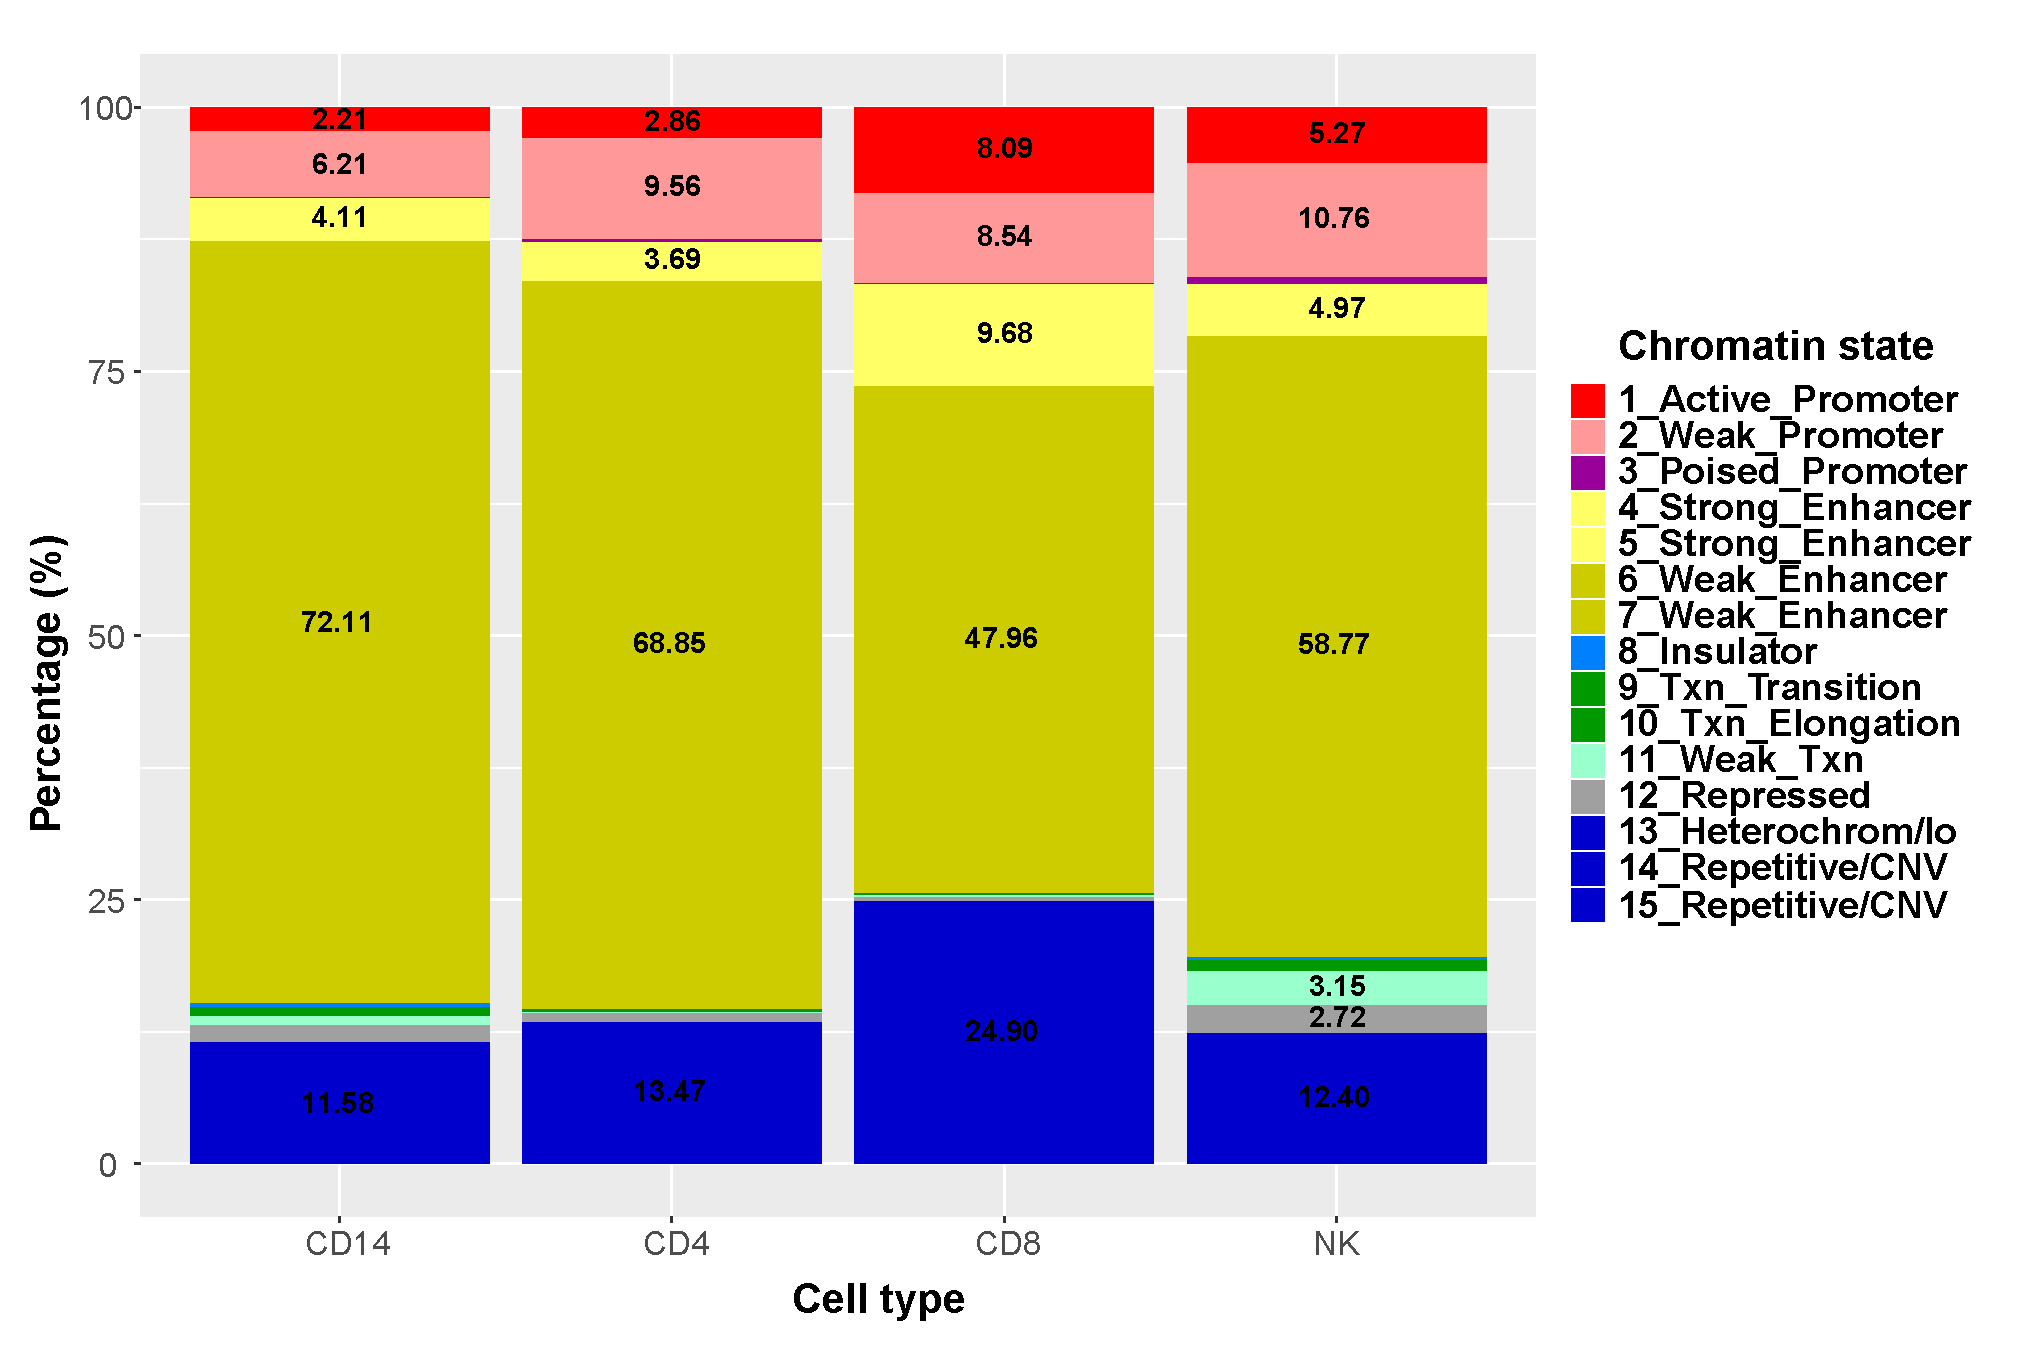
\includegraphics[width=\textwidth]{./Results3/pdfs/ATAC_PSA_DOCS_chromatin_states_stacked_barplot}
\caption{}
\end{subfigure}
\caption[Annotation with genomic regions and chromatin states of the PsA DOCs from the four cell types differential analysis.]{\textbf{Annotation with genomic regions and chromatin states of the PsA DOCs from the four cell types differential analysis.} xxxx}
\label{figure:PsA_FAST_ATAC_DOCS_annotation}
\end{figure}


%Try to overlap the enhancer FANTOM data to id those regions whith evidence of eRNA expression
The functional relevance of the differential chromatin accessibility in terms of regulation of gene expression was further investigated by integration of the eRNA data from the FANTOM5 project. Statistically significant enrichment for robust and permissive enhancers was found for the DARs in all four cell types (Figure \ref{figure:PSA_FANTOM}).  Moreover, DARs from all four cell types also presented significant enrichment for the corresponding cell type eRNA set. The proportion of DARs overlapping the appropriate cell type set of expressed eRNAs ranged between 19.8\% (83 open in SF and 160 open in PB) in NK and 31.8\% (83 open in SF and 160 open in PB) in CD4$^+$ cells.


\begin{figure}[htbp]
\centering
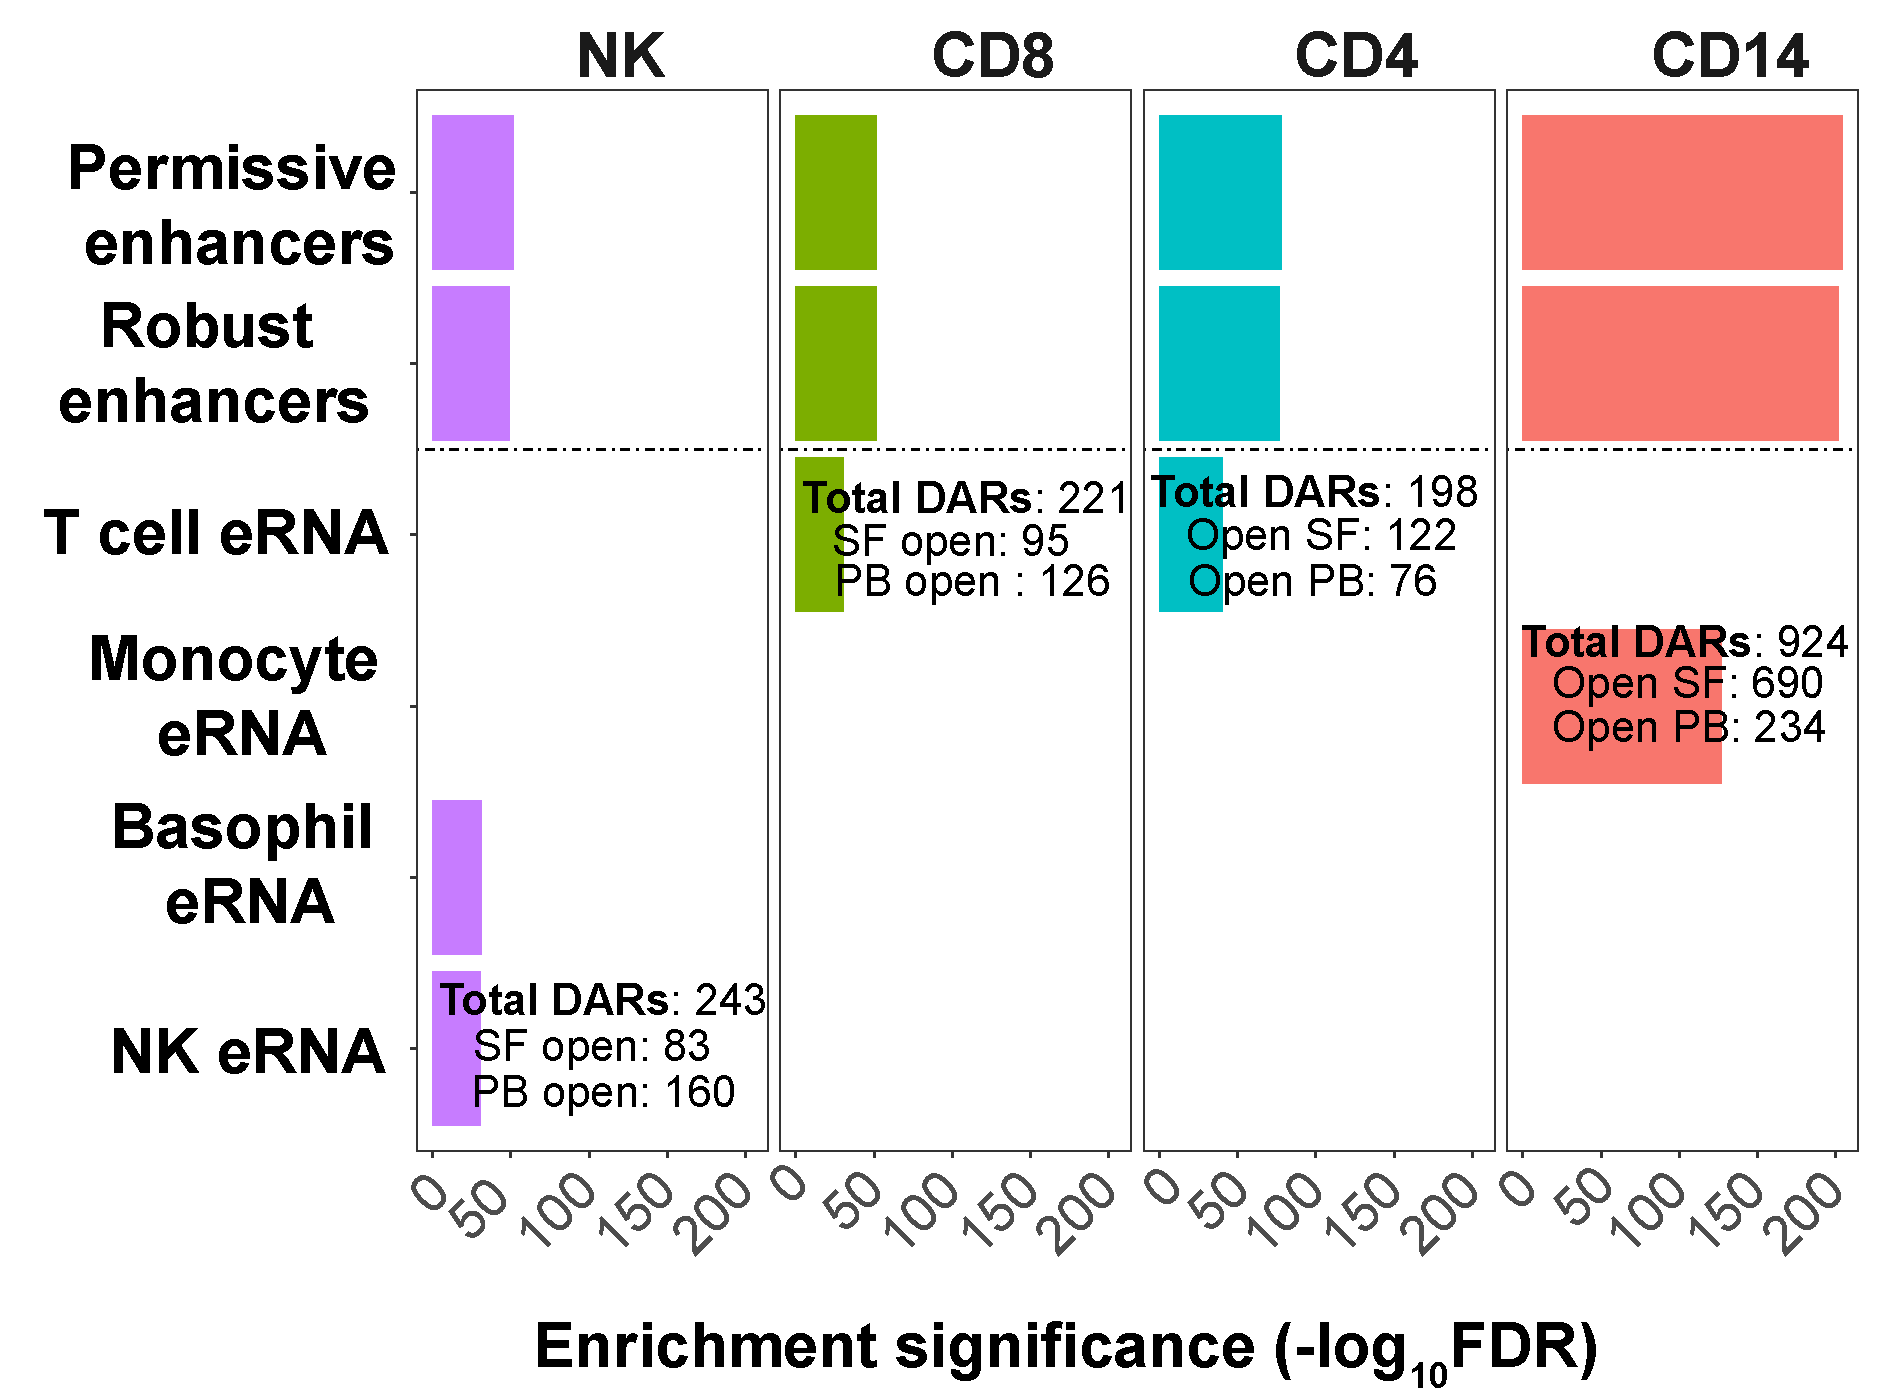
\includegraphics[width=0.6\textwidth]{./Results3/pdfs/ATAC_PsA_FANTOM_enhancer_enrichment_all_cell_types}
\caption[Enrichment of PsA DARs for the FANTOM5 eRNA dataset.]{\textbf{Enrichment of PsA DOCs for the FANTOM5 eRNA dataset.} Robust enhancers have been defined as those detected at the genome-wide significant level in at least one primary cell type or tissue. Permissive enhancers are all detected eRNAs but not passing genome-wide filtering criteria \parencite{Andersson2014}. Robust enhancers represent a subset of the permissive.}
\label{fig:PSA_FANTOM}
\end{figure}

From the differential analysis between SF and PB, a number of DARs were overlapping a gene body (Table \ref{tab:PSA_DOCs_gene_body}). Interestingly, the majority were located within introns instead of untranslated regions (UTRs) and have also been annotated as weak or strong enhancers according to the cell type specific chromatin segmentation map. 

%Similarly, more accessible chromatin in SF compared to PB was identified in five regions of the \textit{IL15} gene, annotated as promoter and enhancers in CD14$^+$ monocytes. 
% Check differences at both gene locations were CD14$^+$ cell type specific is this region HiC annotated with the gene? and maybe include example overlapping eRNA
%e.g LMNA4 which is CD14 cell specific and more expressed in SF in Dolcino paper. Maybe use it later

\begin{table}[htbp]
%\setlength{\tabcolsep}{20pt} only to stretch the columns if you want
%\renewcommand{\arraystretch}{1.5}
\centering
\begin{tabular}{@{} c c c c c}
\toprule
\textbf{Cell type} & \textbf{DARs in gene body} &  \textbf{Gene with $>$ one DAR} &\textbf{Enhancers} & \textbf{Introns} \\
\midrule
\midrule
CD14$^+$ & 2,357 & 744 & 1,775 & 1,920 \\
CD4$^+$ & 700 & 99 & 504 & 577 \\
CD8$^+$ & 831 & 118 & 503 & 666 \\
NK   & 1,246 & 235 & 782 & 937 \\   
\bottomrule
\end{tabular}
\medskip %gap
\caption[Annotation of gene body DARs in four cell types from PsA samples.]{\textbf{Annotation of gene body DARs in four cell types from PsA samples.}xxxx}
\label{tab:PSA_DOCs_gene_body}
\end{table}

For example, NK analysis identified a PB open DAR located in an intron of the \textit{VAV3} gene and also significantly expressed as eRNA (Figure \ref{figure:PsA_FAST_ATAC_gene_boy_DOCS_CD14_NK} a). Additionally, a number of gene entities contained more than one DAR, showing the same direction of chromatin accessibility between SF and PB. For example, in CD14$^+$ two DARs located at the 5' and 3' UTRs of \textit{IL7R} gene were more accessible in SF compared to PB (Figure \ref{figure:PsA_FAST_ATAC_gene_boy_DOCS_CD14_NK} b). 

\bigskip
\begin{figure}[H]
\centering
\begin{subfigure}[b]{0.70\textwidth}
\centering 
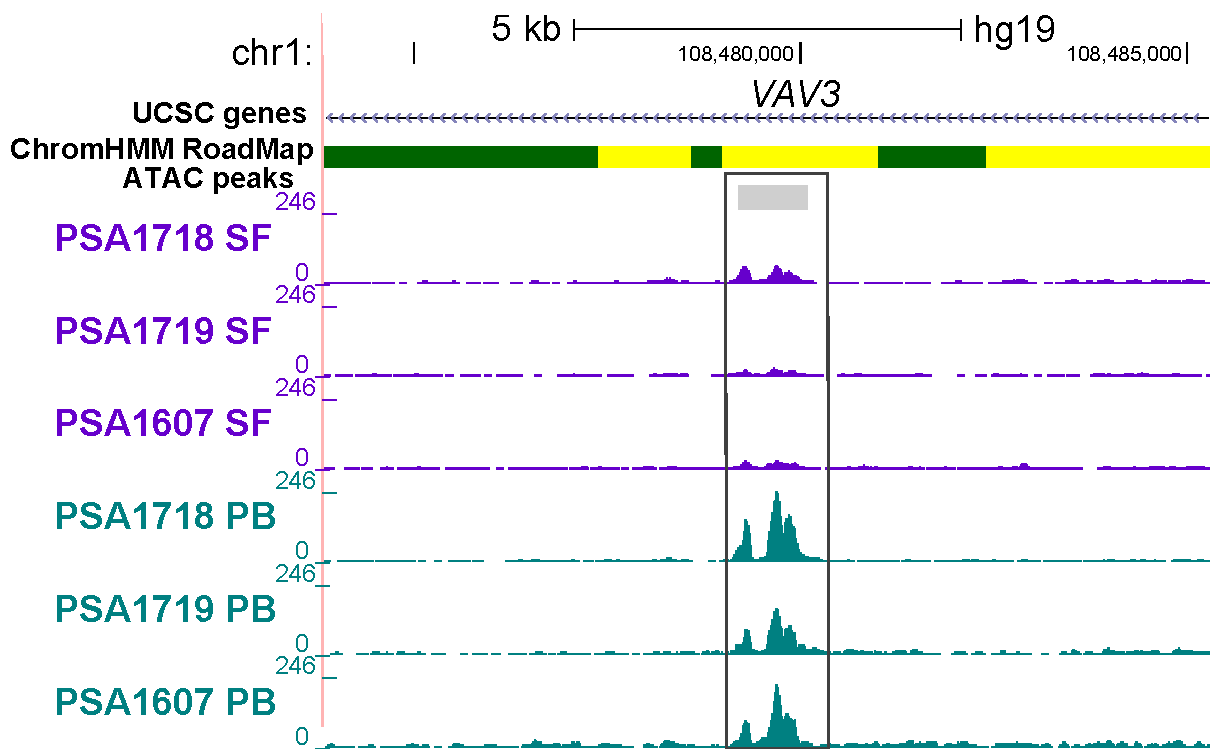
\includegraphics[width=\textwidth]{./Results3/pdfs/ATAC_PSA_NK_VAV3}
\caption{}
\end{subfigure}
~
\begin{subfigure}[b]{0.70\textwidth} 
%the [b] prevents offset in subcaptions
\centering
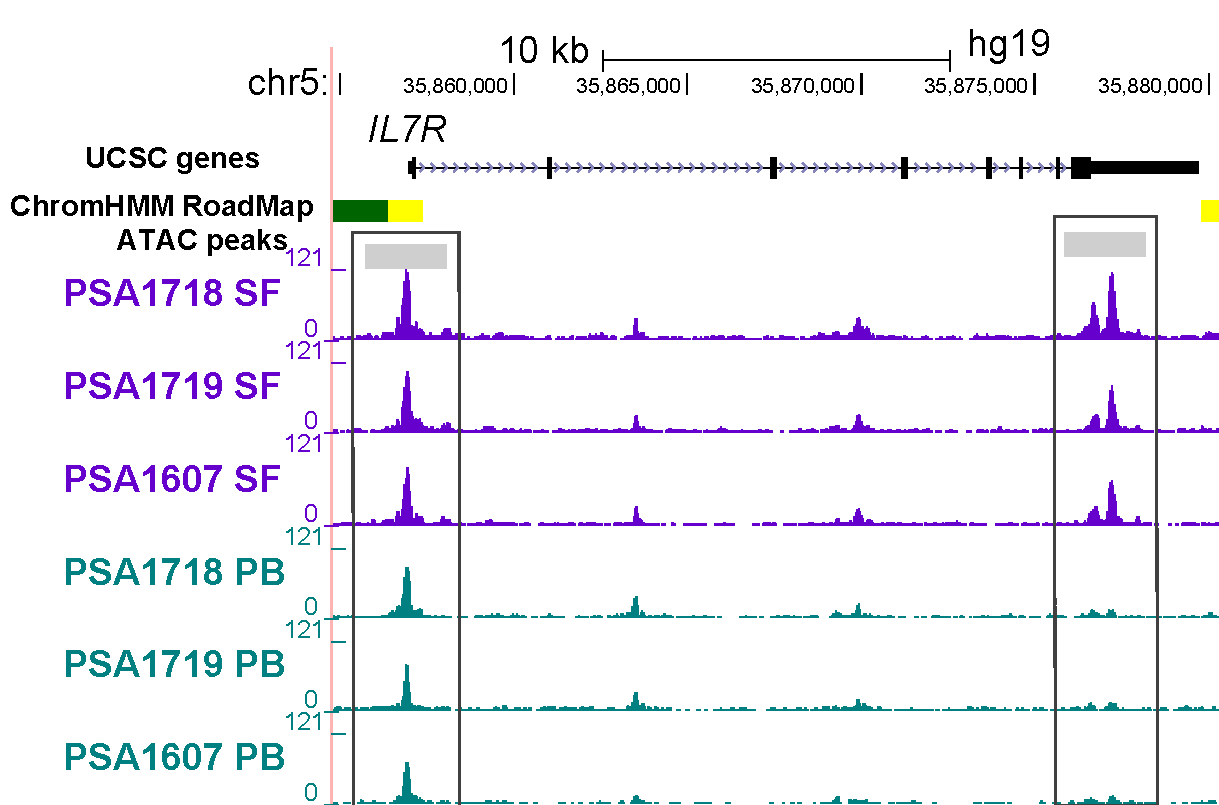
\includegraphics[width=\textwidth]{./Results3/pdfs/ATAC_PSA_CD14_IL7R}
\caption{}
\end{subfigure}
\caption[Differentially accessible regions located within gene bodies in CD14$^+$ monocytes and NK cells from PsA patients.]{\textbf{Differentially accessible regions located within gene bodies in CD14$^+$ monocytes and NK cells from PsA patients.} xxxx}
\label{figure:PsA_FAST_ATAC_gene_boy_DOCS_CD14_NK}
\end{figure}

% GWAS overlap maybe indicate an example in CD14 that can be relevant with pathway analysis
The relevance of the differences in chromatin accessibility in the context of psoriasis and PsA GWAS hits was also addressed. Enrichment analysis of psoriasis and PsA GWAS hits for the DARs in each cell type was performed using XGR co-localisation and permutation analysis. At the SNP level, no significant enrichment was reported between DARs and GWAS lead SNPs and those in LD r$^2$$\geq$8. When the enrichment analysis was performed for the psoriasis and PsA LD blocks, significant enrichment (2-fold enrichment and empirical p-val 0.043) was observed only for the CD14$^+$ DARs.
%
%

\subsection{Pathway enrichment analysis highlights tissue functional differences in chromatin accessibility}

Pathway enrichment analysis was conducted separately for SF open DARs and PB open DARs in each cell type. Gene annotation of the DARs was performed by physical proximity, as detailed in Chapter \ref{ch:Mat}. Despite commonalities, differences in significant enriched pathways (FDR$<$0.01 or 0.05) were also identified within the same cell type between SF and PB open DARs (Figure \ref{figure:PSA_ATAC_pathway_analysis_all_DOC}). In CD14$^+$ monocytes SF open DARs presented enrichment for pathways involved in regulation of immunity, inflammation and cell survival such as the NF-$\kappa$B pathway and cytokine related pathways, including IL-2 and IL-3, 5 and granulocyte-macrophage colony–stimulating factor (GM-CSF) signalling (Figure \ref{figure:PSA_ATAC_pathway_analysis_all_DOC} a). 

mCD4$^+$ SF open DARs compared to PB open DARs showed enrichment for TCR signalling as well as chemokine signalling, which included DARs in proximity to IFN-$\gamma$, IL-2 receptor alpha (\textit{IL2RA}) and IL-5 receptor alpha (\textit{IL5RA}), amongst others (Figure \ref{figure:PSA_ATAC_pathway_analysis_all_DOC} b). The SF open DARs in \textit{IL2R} and \textit{IL5R} may be related to the the IL-2, IL-3 and IL-5 pathway enrichment in CD14$^+$ SF open DARs. Although the T cell signaling pathway appears only enriched for SF open DARs in mCD4$^+$, PB open DARs in this cell type were also enriched for focal adhesion members, also involved in the T cell activation \parencite{Dustin2001}. Enriched pathways for SF or PB open DARs in mCD8$^+$ were only significant when using an FDR$<$0.05 threshold. (Figure \ref{figure:PSA_ATAC_pathway_analysis_all_DOC} c). Interestingly, the G protein coupled receptor (GPCR) signalling was enriched for mCD8$^+$ PB open DARs, consistent with the role of this pathway in mediating the chemotactic recruitment of T cells to the inflammed tissue. mCD8$^+$ SF open DARs showed enrichment for the Wnt signaling pathway involved in the production of memory cells with enhanced proliferative potential and stronger protective capacity \parencite{Boudousqui\'{e}2014,}. 

NK SF open DARs presented enrichment for Fc-gamma receptor (FC$\gamma$R)-mediated phagocytosis that could be triggered by occurrence of monoclonal gammopathy of undetermined significance (MGUS) in PsA patients and consequently induce NK activation (Figure \ref{figure:PSA_ATAC_pathway_analysis_all_DOC} d). Moreover, members of the HIF-1 pathway involved in oxygen homeostasis were also enriched in NK SF open DARs, in line with the hypoxic environment found in joint inflammation. Interestingly, enrichment of open PB DARs in the proximity of NK cell mediated toxicity genes was unveiled. According to FACS analysis, the proportion of NK CD56$\textsuperscript{bright}$ was greater in PB compared to SF in this sample cohort (data not shown). This is consistent with the observed enrichment for NK cytotoxicity in PB open DARs and previous studies demonstrating that CD56$\textsuperscript{bright}$ NK cells are preferentially cytokine producers compared to the tissue resident ones. 
% NK CD56 bright subsets and tissue http://www.jimmunol.org/content/196/7/2923.long
% Production of IgG in PsA http://www.jrheum.org/content/41/12/2421.long
% NK phagocytisis FCgamma R III https://www.ncbi.nlm.nih.gov/pmc/articles/PMC1550276/, https://www.sciencedirect.com/science/article/pii/S0022202X15300373#bb0030, https://www.sciencedirect.com/science/article/pii/S0022202X15300373#bb0185
%Joint hypoxia https://www.ncbi.nlm.nih.gov/pmc/articles/PMC3683428/
%Skin hypoxia https://www.sciencedirect.com/science/article/pii/S0022202X15331328?via%3Dihub

\begin{figure}[H]
\centering
\begin{subfigure}[b]{0.45\textwidth}
\centering 
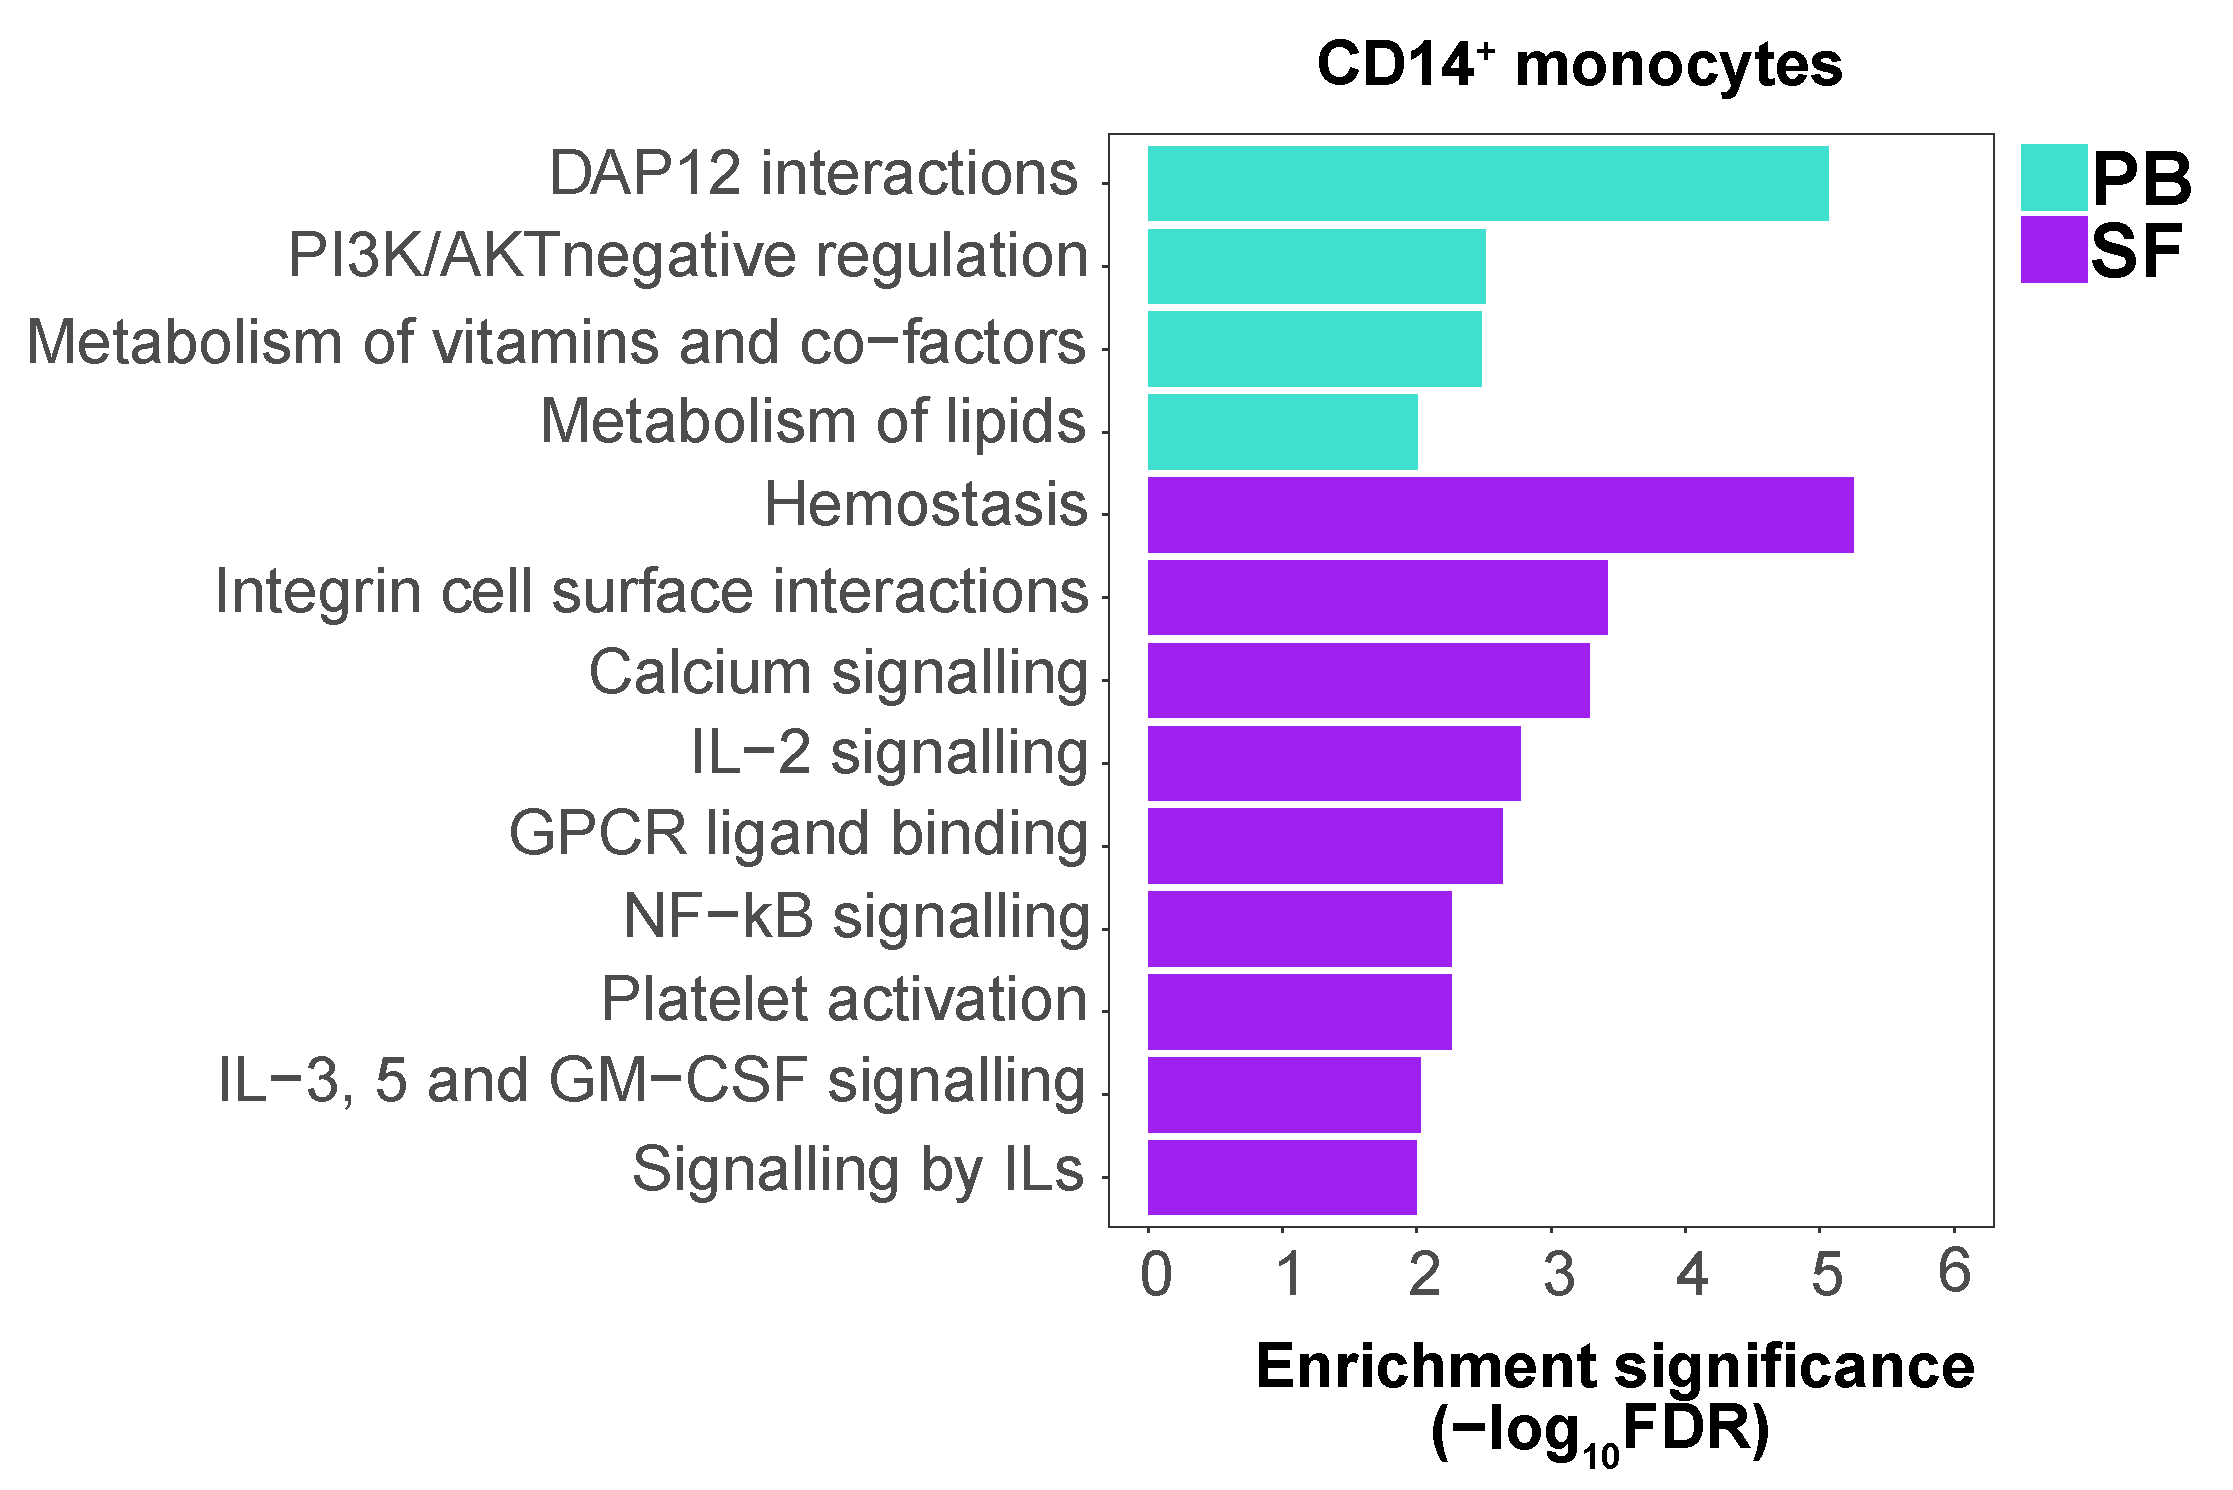
\includegraphics[width=\textwidth]{./Results3/pdfs/ATAC_PSA_CD14_pathways_barplot_all_DOCS_proximity}
\caption{}
\end{subfigure}
~
\begin{subfigure}[b]{0.45\textwidth}
\centering 
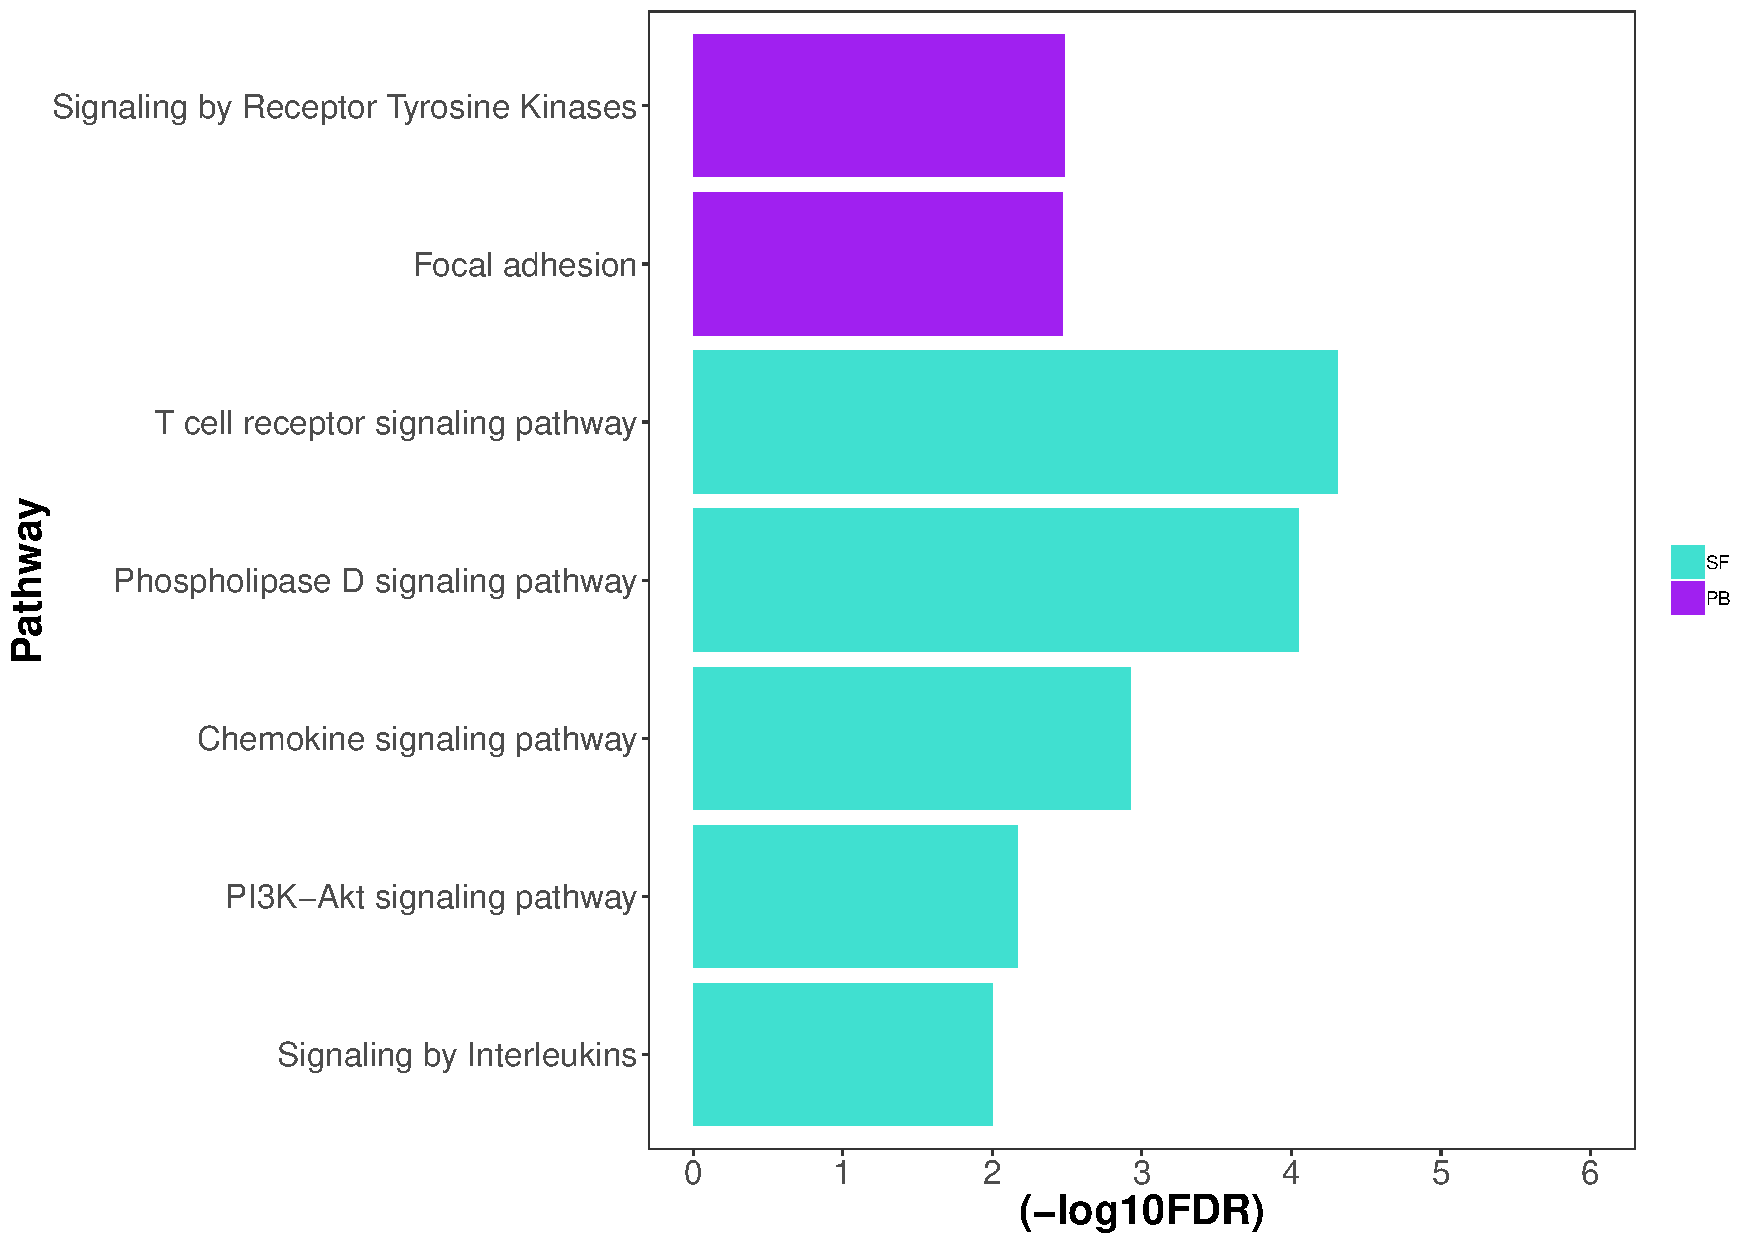
\includegraphics[width=\textwidth]{./Results3/pdfs/ATAC_PSA_CD4_pathways_barplot_all_DOCS_proximity}
\caption{}
\end{subfigure}
~
\begin{subfigure}[b]{0.45\textwidth} 
%the [b] prevents offset in subcaptions
\centering
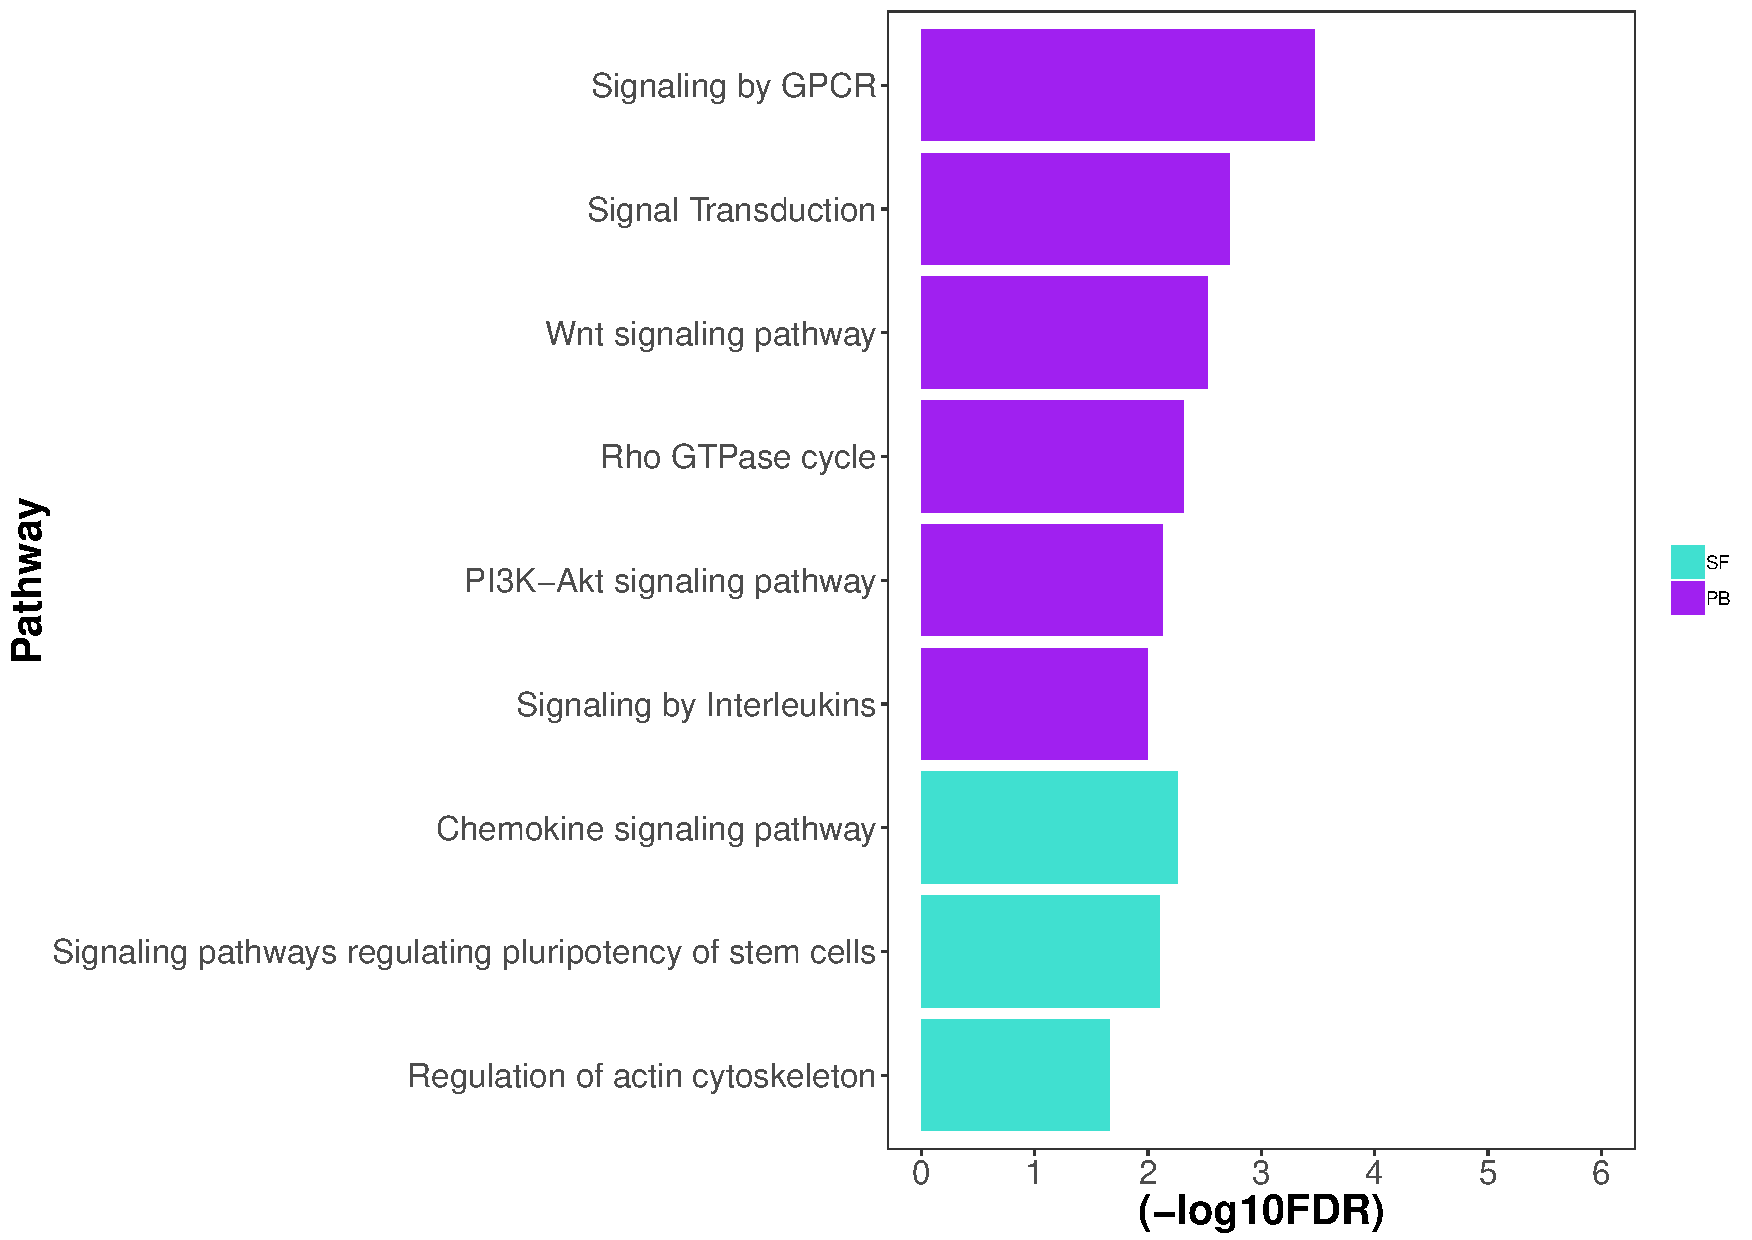
\includegraphics[width=\textwidth]{./Results3/pdfs/ATAC_PSA_CD8_pathways_barplot_all_DOCS_proximity}%
\caption{}
\end{subfigure}
\begin{subfigure}[b]{0.45\textwidth} 
%the [b] prevents offset in subcaptions
\centering
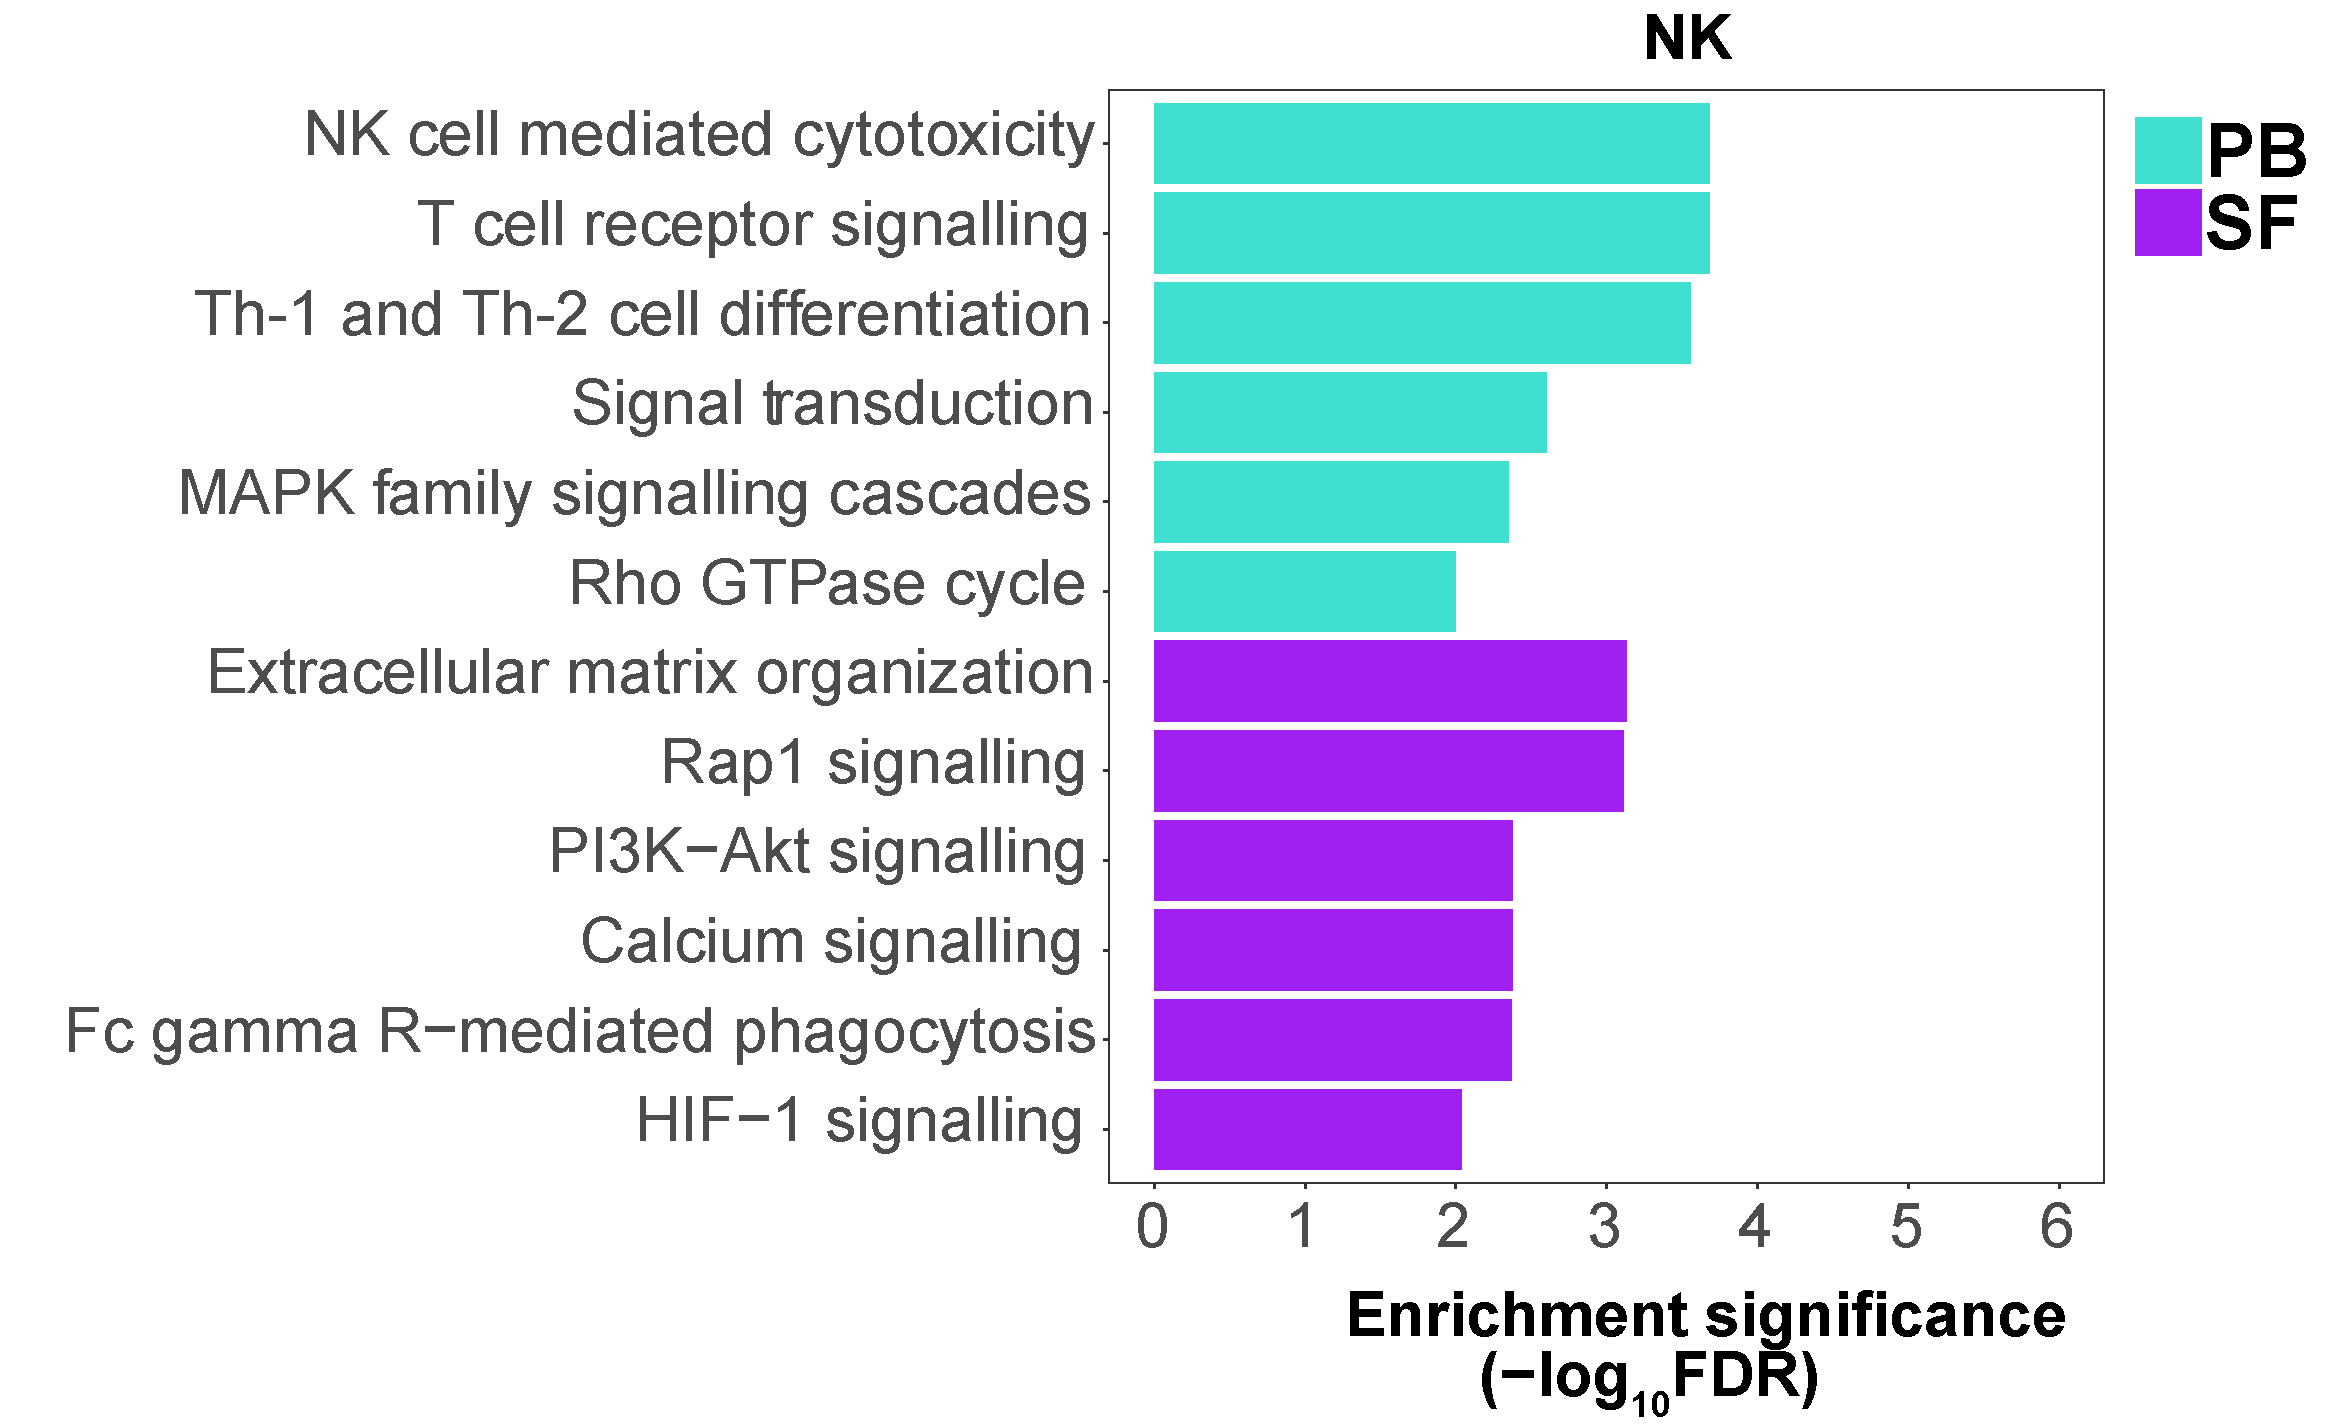
\includegraphics[width=\textwidth]{./Results3/pdfs/ATAC_PSA_NK_pathways_barplot_all_DOCS_proximity}%
\caption{}
\end{subfigure}
\caption[Distinct enriched pathways across SF and PB in CD14$^+$,CD4m$^+$,CD8m$^+$ and NK.]{\textbf{Distinct enriched pathways across SF and PB in CD14$^+$, CD4m$^+$, CD8m$^+$ and NK.} All pathways shown have an FDR $<$0.01.}
\label{figure:PSA_ATAC_pathway_analysis_all_DOC}
\end{figure}


%Decide if table or barplots
%\begin{landscape}
%\begin{center}
%\begin{longtable}[ht]{c c c }
%\caption[Distinct enriched pathways in CD14$^+$, mCD4$^+$, mCD8$^+$ and NK between SF and PB]{\textbf{Distinct enriched pathways in CD14$^+$, mCD4$^+$, mCD8$^+$ and NK between SF and PB.} All pathways shown have an FDR $<$0.01.}
%\\
%\label{table:PSA_ATAC_pathway_analysis_all_DOC} \\
%\toprule
%\textbf{Cell type} & \textbf{SF} & \textbf{PB} \\						
%\midrule
%\midrule
%CD14$^+$ & Hemostasis, Platelet activation, Signaling by VEGF & DAP12 interactions, Metabolism of lipids, \\ 
         %& GPCR ligand binding, IL-2 signaling pathway, & Metabolism of vitamins and co-factors, \\ 
         %& Integrin cell surface interactions,NF-kappa B signaling pathway & Negative regulation of the PI3K/AKT network. \\ 
         %& IL-2 family signaling, IL-3, 5 and GM-CSF signaling. & \\ 
%\midrule
%\textbf{mCD4$^+$} & T cell receptor signaling pathway, Phospholipase D signaling pathway ,& Signaling by Receptor Tyrosine Kinases,\\ 
									%& Chemokine signaling pathway, PI3K-Akt signaling pathway, & Focal adhesion.\\ 
									%& Signaling by interleukins. & \\
%\midrule
%\textbf{mCD8$^+$} & Chemokine signaling pathway, Signaling by GPCR  & Signal transduction, Wnt signaling pathway,\\ 
									%& Signaling pathways regulating pluripotency of stem cells & Rho GTPase cycle, PI3K-Akt signaling pathway, \\ 
									%& Regulation of actin cytoskeleton. & Signaling by interleukins. \\ 
%\midrule
%\textbf{NK$^+$} & Extracellular matrix organization, Rap1 signaling pathway, & Th1 and Th2 cell differentiation, Rho GTPase cycle,\\ 		
								%& Calcium signaling pathway, PI3K-Akt signaling pathway,     & T cell receptor signaling pathway, Signal Transduction,\\ 
								%& Fc gamma R-mediated phagocytosis, HIF-1 signaling pathway. & Natural killer cell mediated cytotoxicity,  \\
								%&                                                            & MAPK family signaling cascades.	\\ 								
%\bottomrule
%\medskip
%\end{longtable}
%\end{center}
%\end{landscape}



%\begin{figure}[htbp]
%\centering
%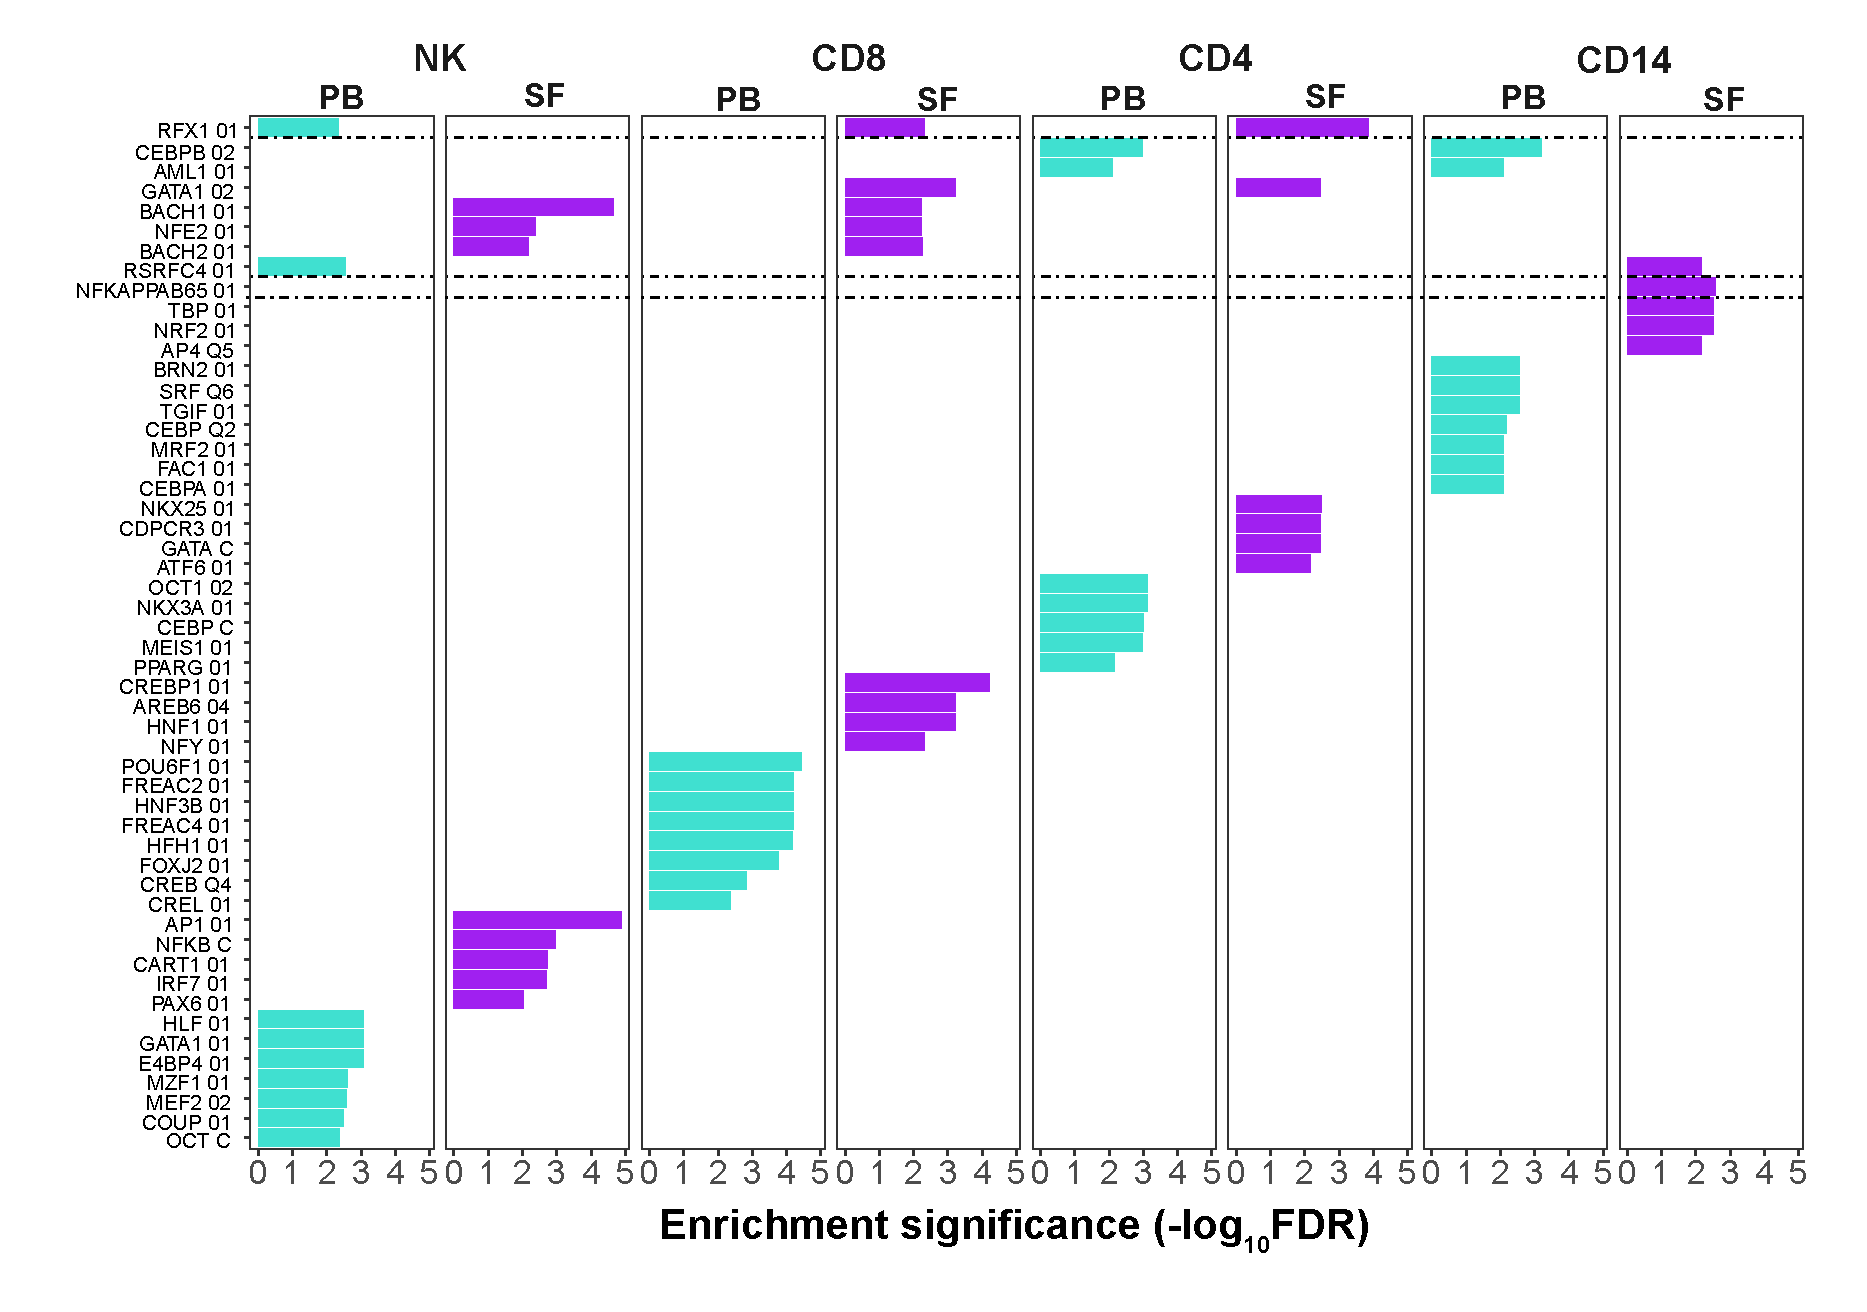
\includegraphics[width=0.8\textwidth]{./Results3/pdfs/ATAC_PSA_enrichment_conserved_TFBS_barplots_cell_type_specific_DOCS_all_cell_types_per_tissue}
%\caption[Enrichment of eRNA cell type-specific PsA DARs for conserved TFBS.]{\textbf{Enrichment of eRNA cell type-specific PsA DARs for conserved TFBS.} xxxx }
%\label{figure:PSA_TFBS}
%\end{figure}



\subsection{Differential gene expression analysis in paired circulating and synovial immune cells}

\subsubsection{Immune-relevant gene expression by qPCR}
%Introductory paragraph to link to ATAC-seq data
Mapping chromatin accessibility represents an informative tool to identify regulatory elements undergoing histone modifications, DNA methylation and TF binding, as previously explained. All those elements are involved in the regulation of gene expression, making the study of chromatin accessibility a good proxy for the inference of gene expression. Nevertheless, the characterisation of the chromatin landscape also presents some limitations, including the discordance between open chromatin and functionality of the regulatory element, shown by CAGE studies, as well as the identification of the target gene regulated by a particular element. 

In order to contextualise the ATAC-seq data, qPCR gene expression analysis for 370 key genes in the inflammatory and autoimmune response was conducted in CD14$^+$ monocytes, mCD4$^+$ and mCD8$^+$ cells isolated from SF and PB of three PsA patients (Table \ref{tab:PSA_datasets_per_sample}). Those appeared as the most abundant cell types in PB and SF from patients and particularly for mCD8$^+$ cells have been shown to expand in PsA inflammed synovium, as previously mentioned. The PCR array represented a cost-effective approach to study gene expression between PB and SF focusing in a relevant subset of genes of notably importance, given the pathophysiological characteristics of PsA. For each cell types, FC in expression was calculated pair-wise for SF respect to PB within each sample for each individual genes (detailed in Chapter \ref{ch:Mat}. Likely due to the small sample size,the majority of the modulated genes between SF and PB lacked of significance (FDR$<$0.05) after multiple testing correction. Therefore, to explore the biological relevance of this data, a less stringent pval$<$0.05 was used as the filtering threshold. 

% Since I am not used corrected pval Hai mentioned that I can not talk about differentially expressed
When considering the significantly modulated genes (pval$<$0.05) in at least one cell type, 
differences in magnitude and reproducibility in FCs were observed across samples and cell types (Figure \ref{figure:PSA_PCR_array_5pcnt_heatmap}). Some of the modulated genes showed up-regulation (FC$>$1.5) in SF compared to PB across the three cell types, for example \textit{FN1}, \textit{SPP1} or \textit{CCL2}, amongst others (Figure \ref{figure:PSA_PCR_array_5pcnt_heatmap} orange box). On the other hand, a number of genes presented reduced expression in SF (FC$<$1) in at least one of the three cell types, including \tetxtit{FOS}, \textit{IL16}, \textit{PPBP} and \textit{TPST1} (Figure \ref{figure:PSA_PCR_array_5pcnt_heatmap} purple box). Also, a number of genes were only consistently modulated in the three CD14$^+$ monocyte samples but not in T cells (Figure \ref{figure:PSA_PCR_array_5pcnt_heatmap} dark blue box). For example, \textit{CCR7} and \textit{IL7R} were up-regulated in SF CD14$^+$ monocytes compared to PB; however the FCs between SF and PB were largely variable across the three patients in mCD4$^+$ and mCD8$^+$. Moreover, differences in the magnitude of FCs across the three cell types were observed for some of the genes modulated in the same direction, for instance \textit{VEGFB} and \textit{CXCR6} (Figure \ref{figure:PSA_PCR_array_5pcnt_heatmap_New} green box).

\begin{landscape}
\begin{figure}[H]
\centering
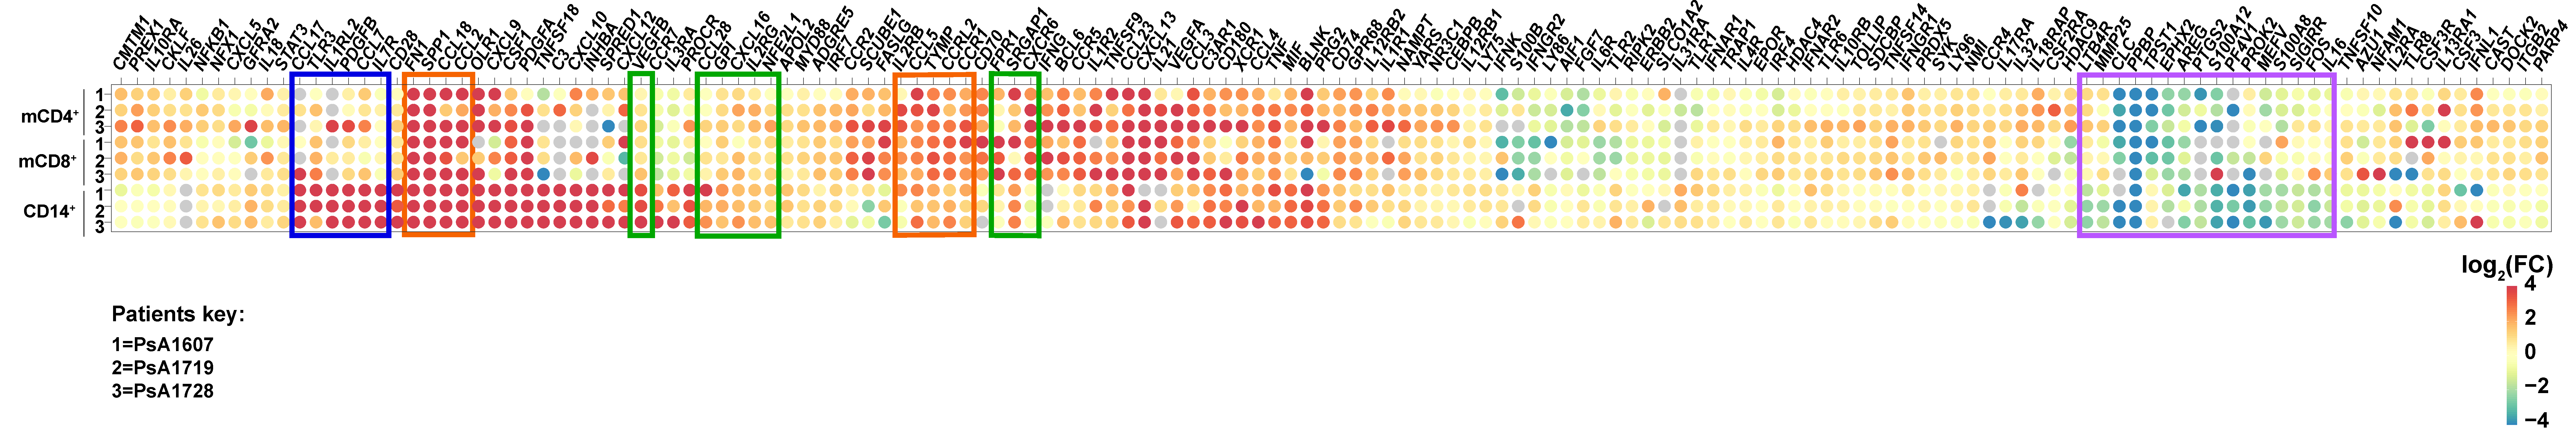
\includegraphics[width=1.5\textwidth]{./Results3/pdfs/PCR_array_PSA_SF_vs_PB_filtered_5_percent_genes_heatmap_New}
\caption[Representation of the FC in gene expression between SF and PB for the significant genes (pval$<$0.05) in at least one of the cell types.]{\textbf{Representation of the FC in gene expression between SF and PB for the significant genes (pval$<$0.05) in at least one of the cell types.} xxxx }
\label{figure:PSA_PCR_array_5pcnt_heatmap}
\end{figure}
\end{landscape}


Filtering of all the genes tested for expression in the qPCR array based on both, statistical significance (pval$<$0.05) and FCs (abs FC$>$1.5), revealed that CD14$^+$ monocytes and mCD8$^+$ presented greater number of significantly modulated genes (70 and 73, respectively) compared to mCD4$^+$ cells (46 genes) (Figure \ref{figure:PSA_PCR_array_vulcano_plots} a, b and c). For the three analysed cell types, the majority of modulated immune genes presented up-regulation in the SF (Figure \ref{figure:PSA_PCR_array_vulcano_plots} a, b and c). For example, 56 out of the 70 significantly modulated genes in CD14$^+$ monocytes showed a mean FC$>$1.5 versus the 14 genes with mean FC$<$1.5 (Figure \ref{figure:PSA_PCR_array_vulcano_plots} a).



% May need a bit more of biology there
\begin{figure}[htbp]
\centering
\begin{subfigure}{0.6\textwidth}
\centering
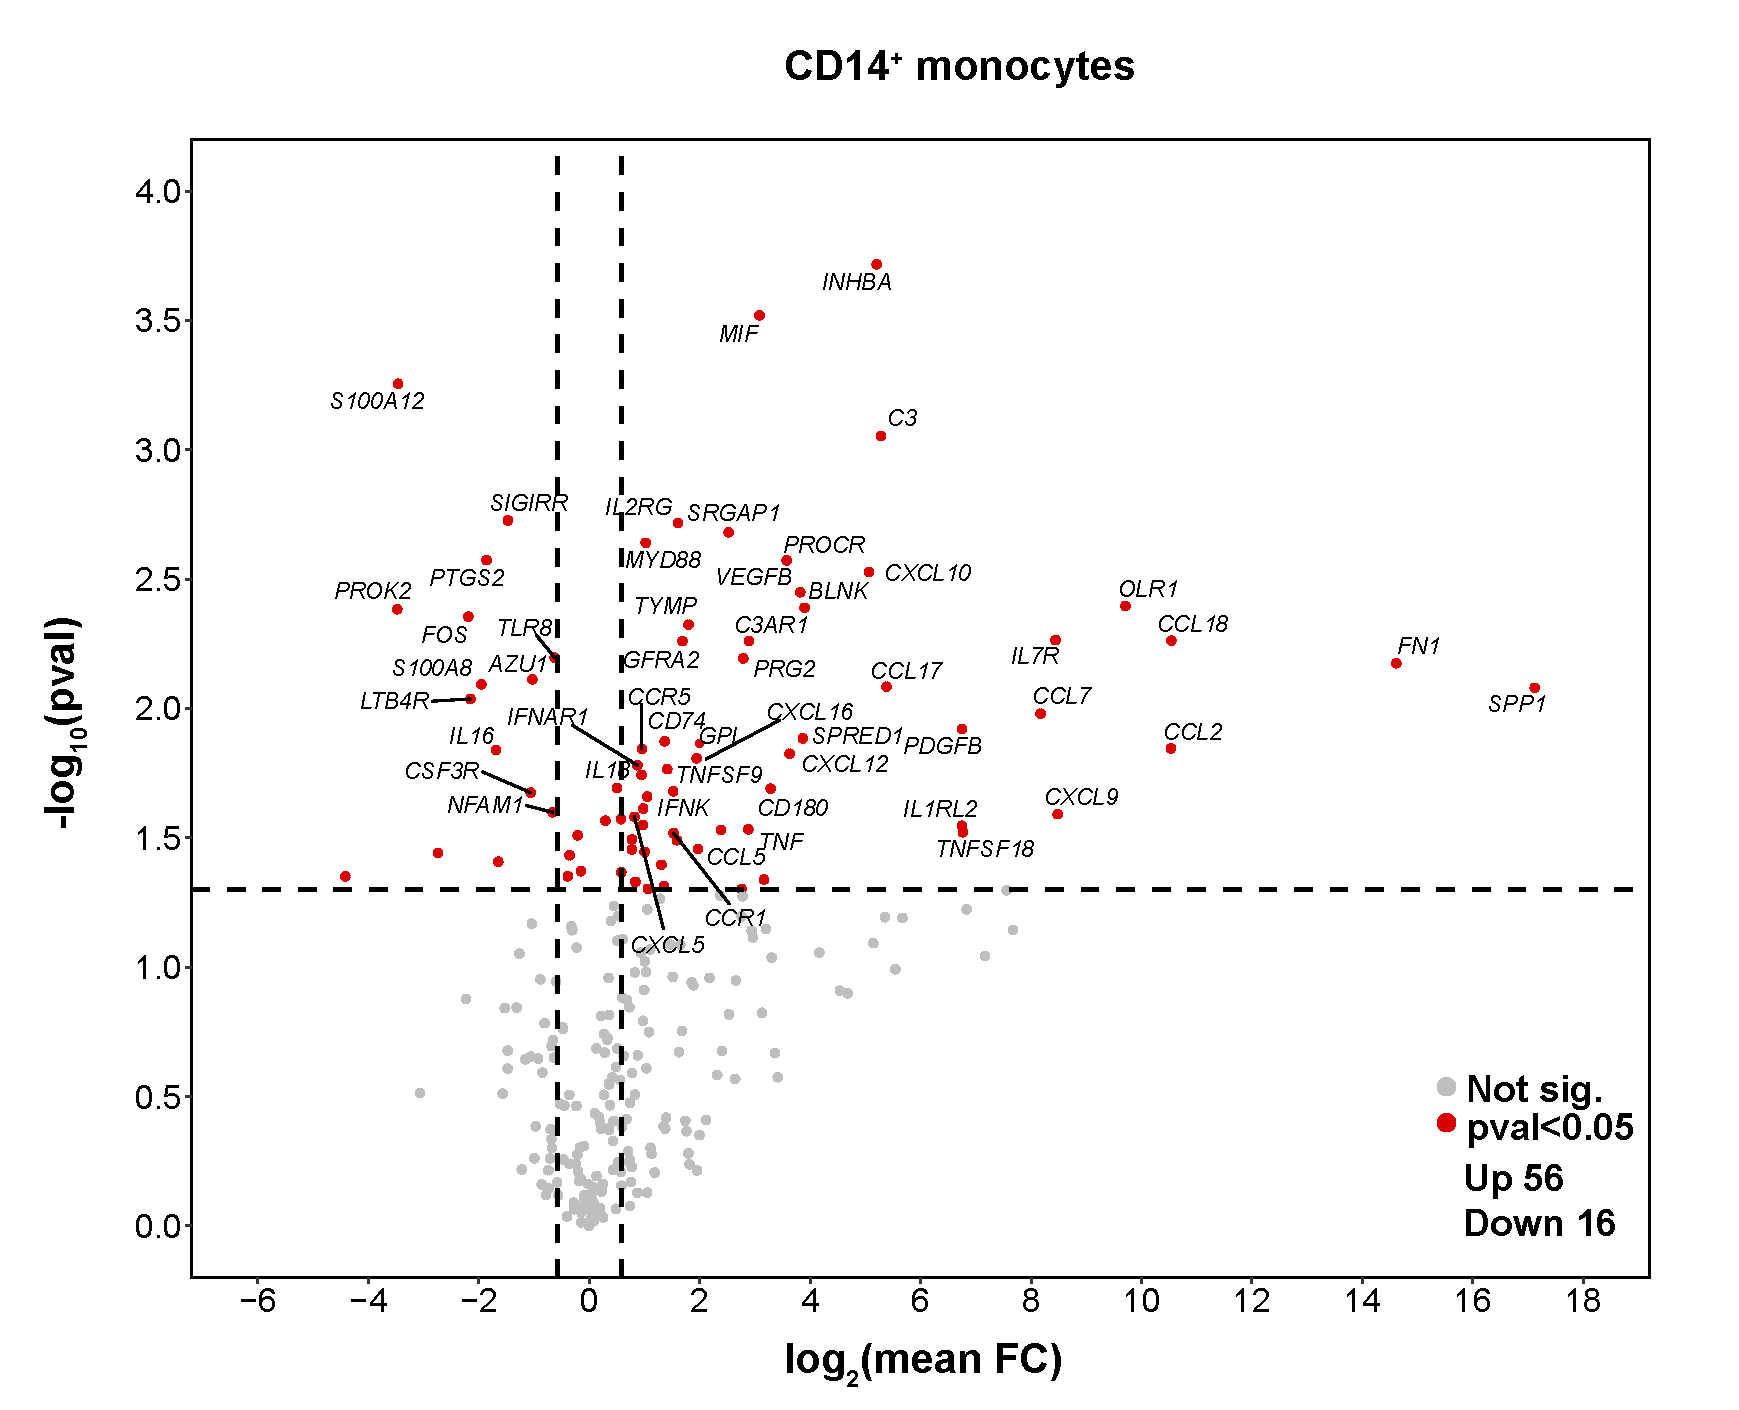
\includegraphics[width=\textwidth]{./Results3/pdfs/PSA_CD14_vulcano_plot_PCR_array_mean_FC}
\caption{\textbf{}}
% The percentage sign indicated that the other subfig goes side by side
\end{subfigure} \\
\begin{subfigure}{0.6\textwidth}
\centering
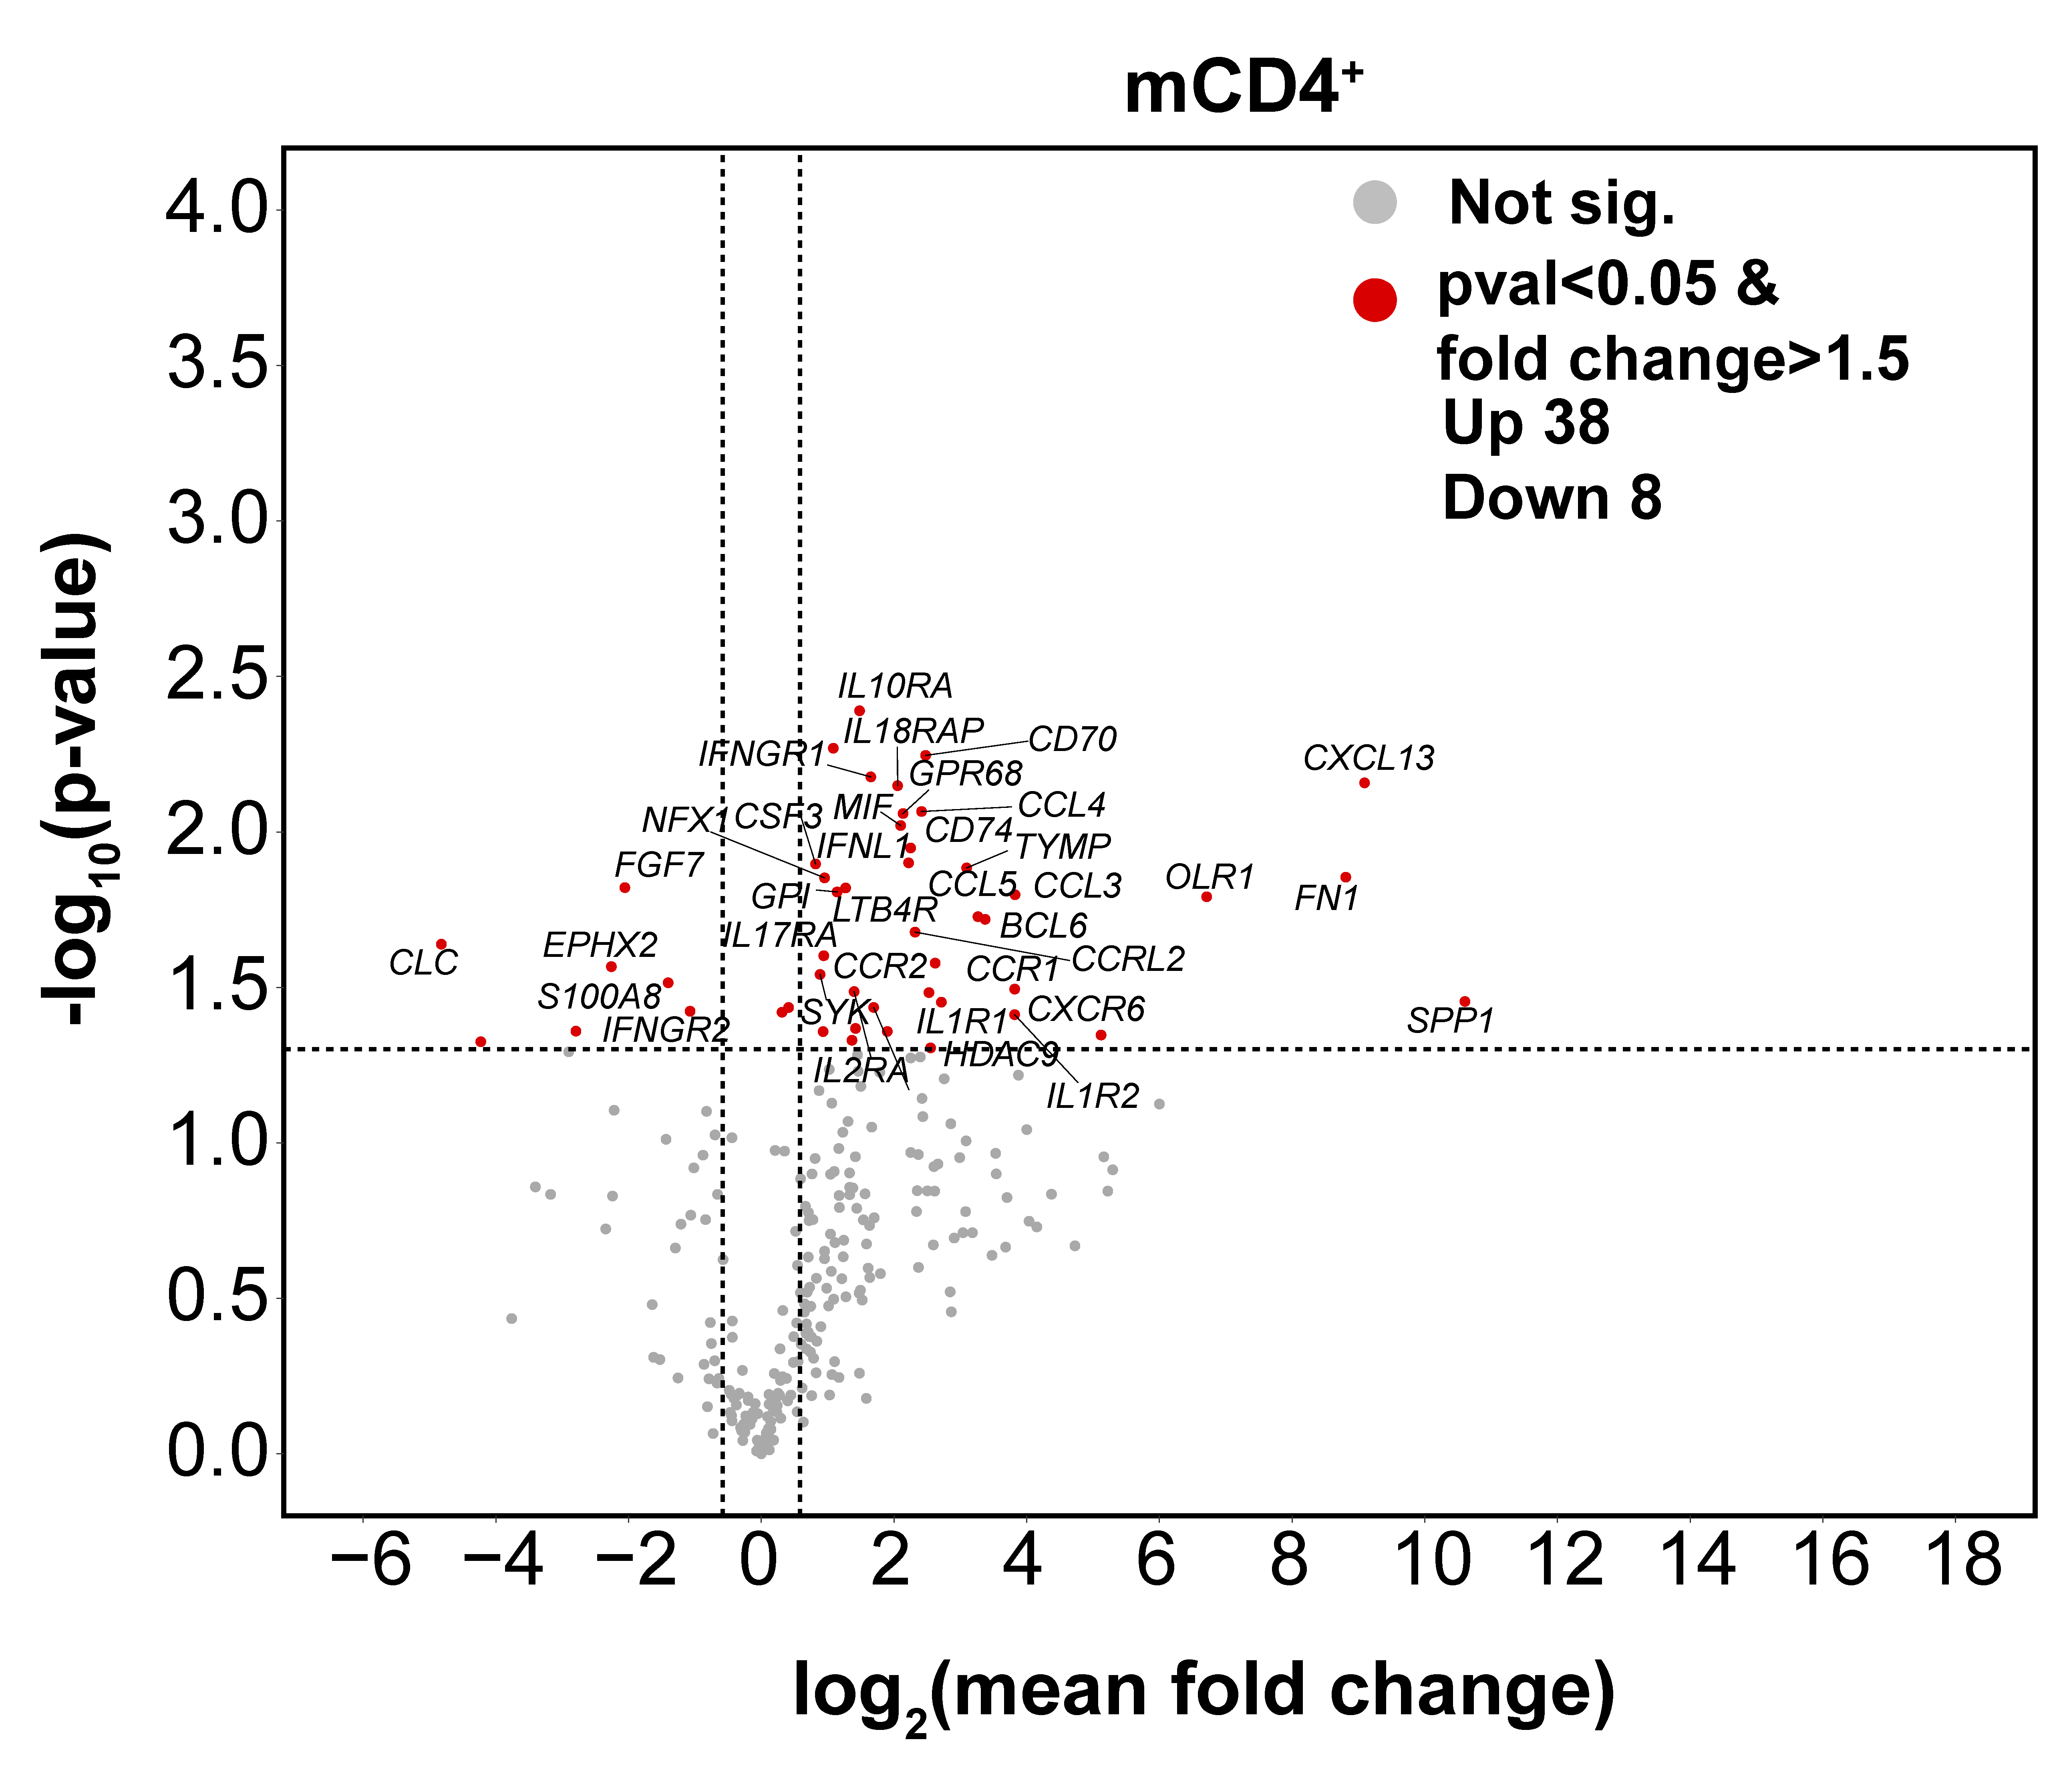
\includegraphics[width=\textwidth]{./Results3/pdfs/PSA_CD4_vulcano_plot_PCR_array_mean_FC}
\caption{\textbf{}}
\end{subfigure} %
\begin{subfigure}{0.6\textwidth}
\centering
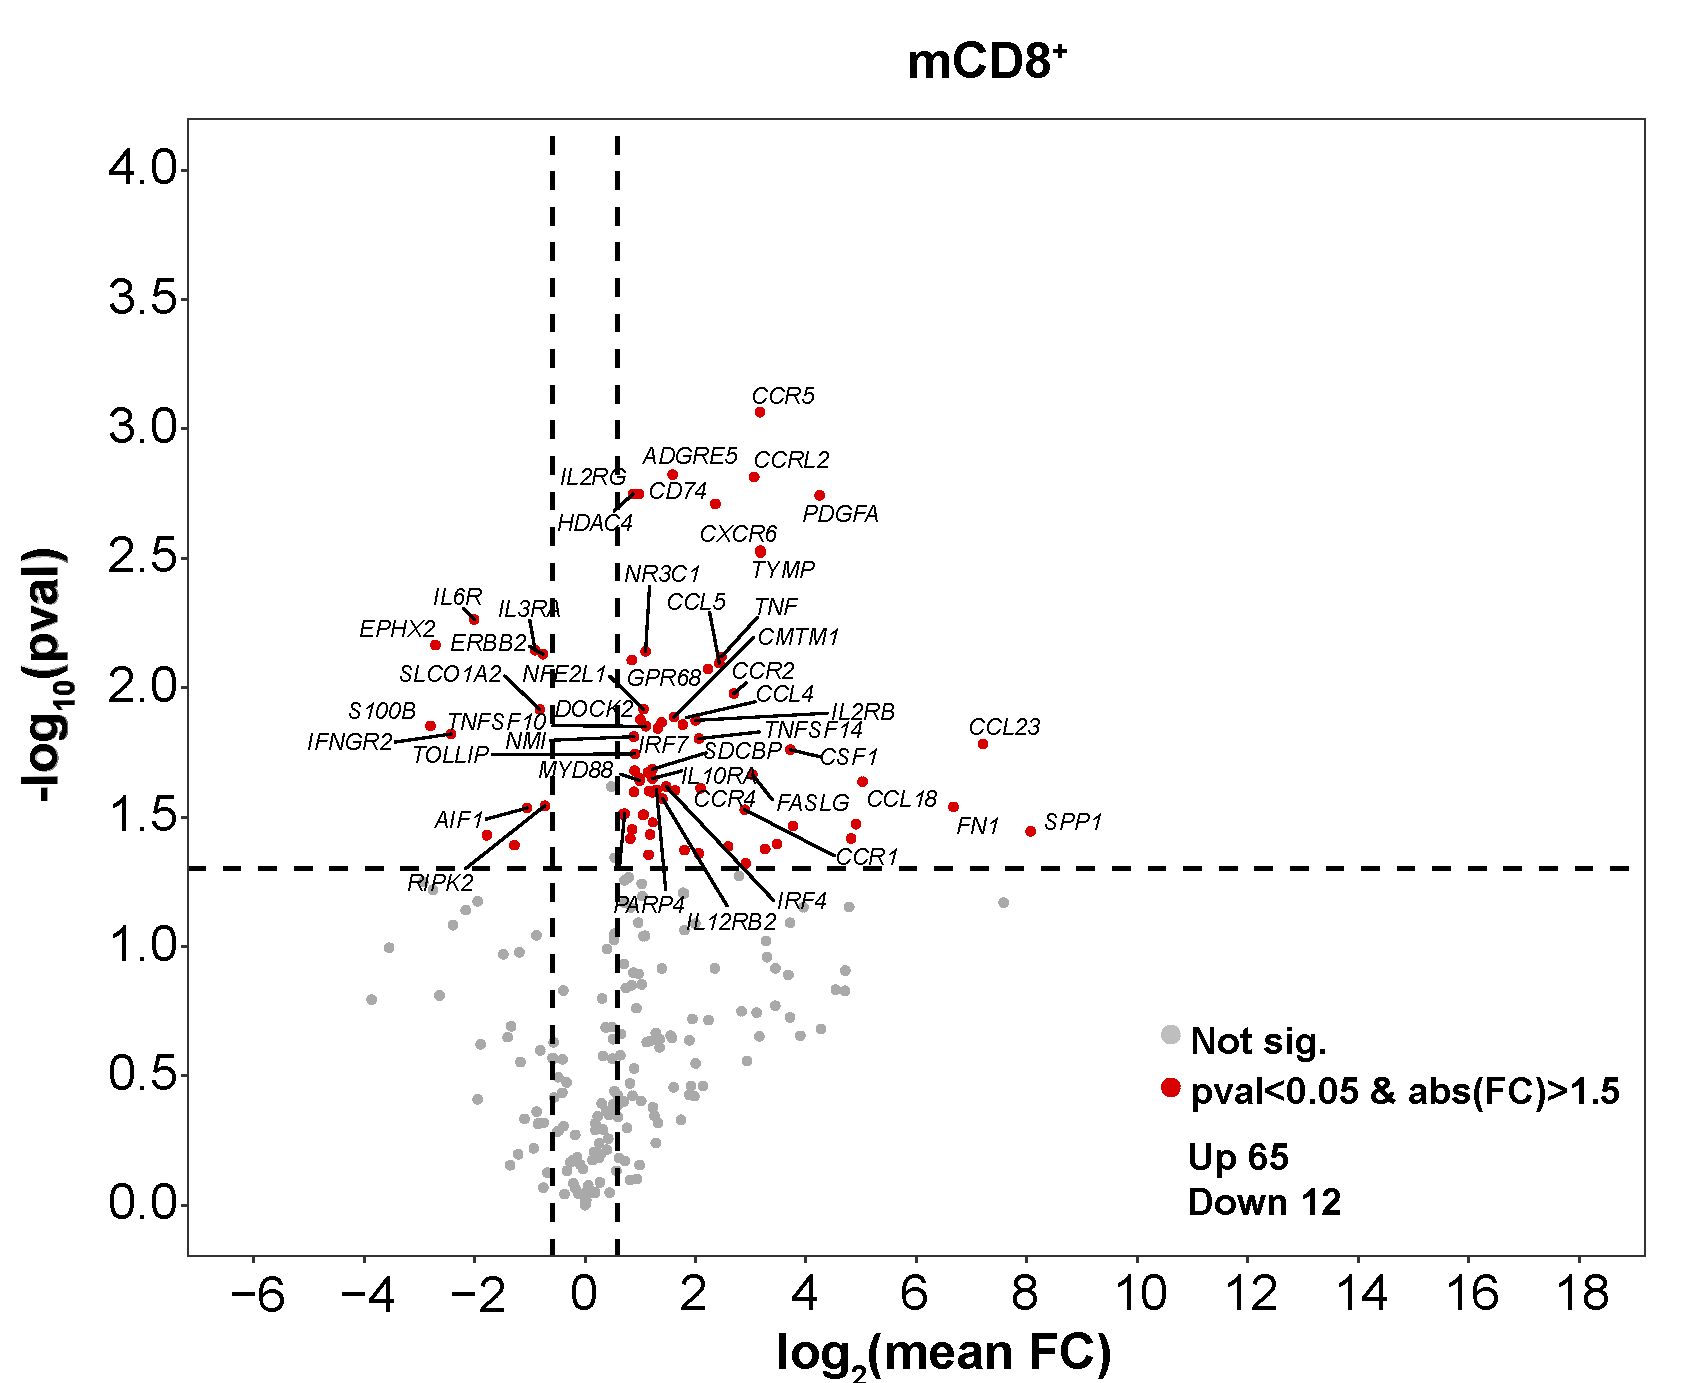
\includegraphics[width=\textwidth]{./Results3/pdfs/PSA_CD8_vulcano_plot_PCR_array_mean_FC}
\caption{\textbf{}}
\end{subfigure}
\caption[Gene expression changes in immune-relevant genes between SF and PB in CD14$^+$ monocytes, mCD4$^+$ and mCD4$^+$ cells.]{\textbf{Gene expression changes in immune-relevant genes between SF and PB in CD14$^+$ monocytes, mCD4$^+$ and mCD4$^+$ cells.}}
\label{figure:PSA_PCR_array_vulcano_plots}
\end{figure} 


\subsubsection{Correlation between gene expression and chromatin accessibility}
% ATAC overall overlap
Amongst the significantly modulated genes (based on pval and FC cut-offs) between SF and PB, overlap with DARs were observed for the three cell types (Table \ref{tab:PSA_gene_expression_ATAC_overlap}). In CD14$^+$ monocytes, 13 out of the 56 significantly up-regulated genes in SF overlapped with SF open DARs. 


\begin{table}[htbp]
%\setlength{\tabcolsep}{20pt} only to stretch the columns if you want
%\renewcommand{\arraystretch}{1.5}
\centering
\begin{tabular}{@{} c c c}
\toprule
\textbf{Cell type} & \textbf{Genes upregulated and}        &  \textbf{Genes downregulated and} \\
                   & \textbf{overlapping open chromatin}   &  \textbf{overlapping closed chromatin} \\
									 &	\textbf{in SF}				               &  \textbf{in SF} \\
\midrule
\midrule
          & 13 (\textit{BLNK}, \textit{CCL2$^\ast$}, \textit{CCR1$^\ast$}, \textit{CD180}, & 2 (\textit{FOS}, \textit{PROK2$^\ast$}) \\      CD14$^+$  & \textit{CXCL10}, \textit{FN1}, \textit{IL18}, \textit{IL31RA$^\ast$},    & \\
monocytes & \textit{IL7R$^\ast$}, \textit{NFKB1$^\ast$}, \textit{PRG2}, \textit{SRGAP1}, & \\
				  & \textit{STAT3}) & \\
				
\midrule
mCD4$^+$ & 3 (\textit{CXCL13}, \textit{CXCR6$^\ast$}), \textit{IL2RA}& 0 \\

\midrule
mCD8$^+$ & 6 (\textit{CCL3}, \textit{CCR2}, \textit{CCR5} ,\textit{IRF4} & 1 (\textit{EPHX2}) \\
         & \textit{TNFSF10}, \textit{YARS}) & \\

\bottomrule
\end{tabular}
\medskip %gap
\caption[Immune genes with significant modulated expression in SF and proximal to a DAR in Fast-ATAC.]{\textbf{Immune genes with significant modulated expression in SF and proximal to a DAR in Fast-ATAC.} An overlap is defined by significant change in expression (pval$<$0.05) of a particular gene where there is also a proximal DAR showing changes in chromatin accessibility in the same direction. ($^\ast$) indicates that the proximal DAR overlapping an eRNA identified by FANTOM5 project in that particular cell type (see subsection Characterisation of the differential accessible chromatin regions).}
\label{tab:PSA_gene_expression_ATAC_overlap}
\end{table}

For example, the greater chromatin accessibility at the \textit{IL7R} 5' and 3' UTR, previously shown (Figure \ref{figure:PsA_FAST_ATAC_gene_boy_DOCS_CD14_NK} b) correlated with greater mRNA expression in SF CD14$^+$ monocytes compared with PB. Another relevant example is the \textit{FN1} gene, involved in cell adhesion, migration and osteoblast biology. Up-regulated expression in synovial biopsies compared to PB has already been reported \parencite{Dolcino2015}. In this cohort, \textit{FN1} expression was up-regulated in SF for all three cell types with the greater FC found in CD14$^+$ monocytes (Figure \ref{figure:PSA_PCR_array_vulcano_plots} a), concomitantly with more accessible chromatin at the promoter and 3' UTR of the gene (Figure \ref{figure:PSA_CD14_ATAC_FN1}). Lesser overlap between up-regulated gene expression and open chromatin in SF compared to PB was observed in mCD4$^+$ and mCD8$^+$ (6 and 3 hits, respectively). Regarding significantly down-regulated genes, only CD14$^+$ monocytes and mCD8$^+$ presented overlap with proximal less accessible chromatin regions in SF (2 and 1, respectively). 
%decide which example to use: I have included IL7R in monocytes and maybe could use FN1 to complete
	%Example expression in CD14 FOS,FN1,CCL2,CXCL10
	
\begin{figure}[htbp]
\centering
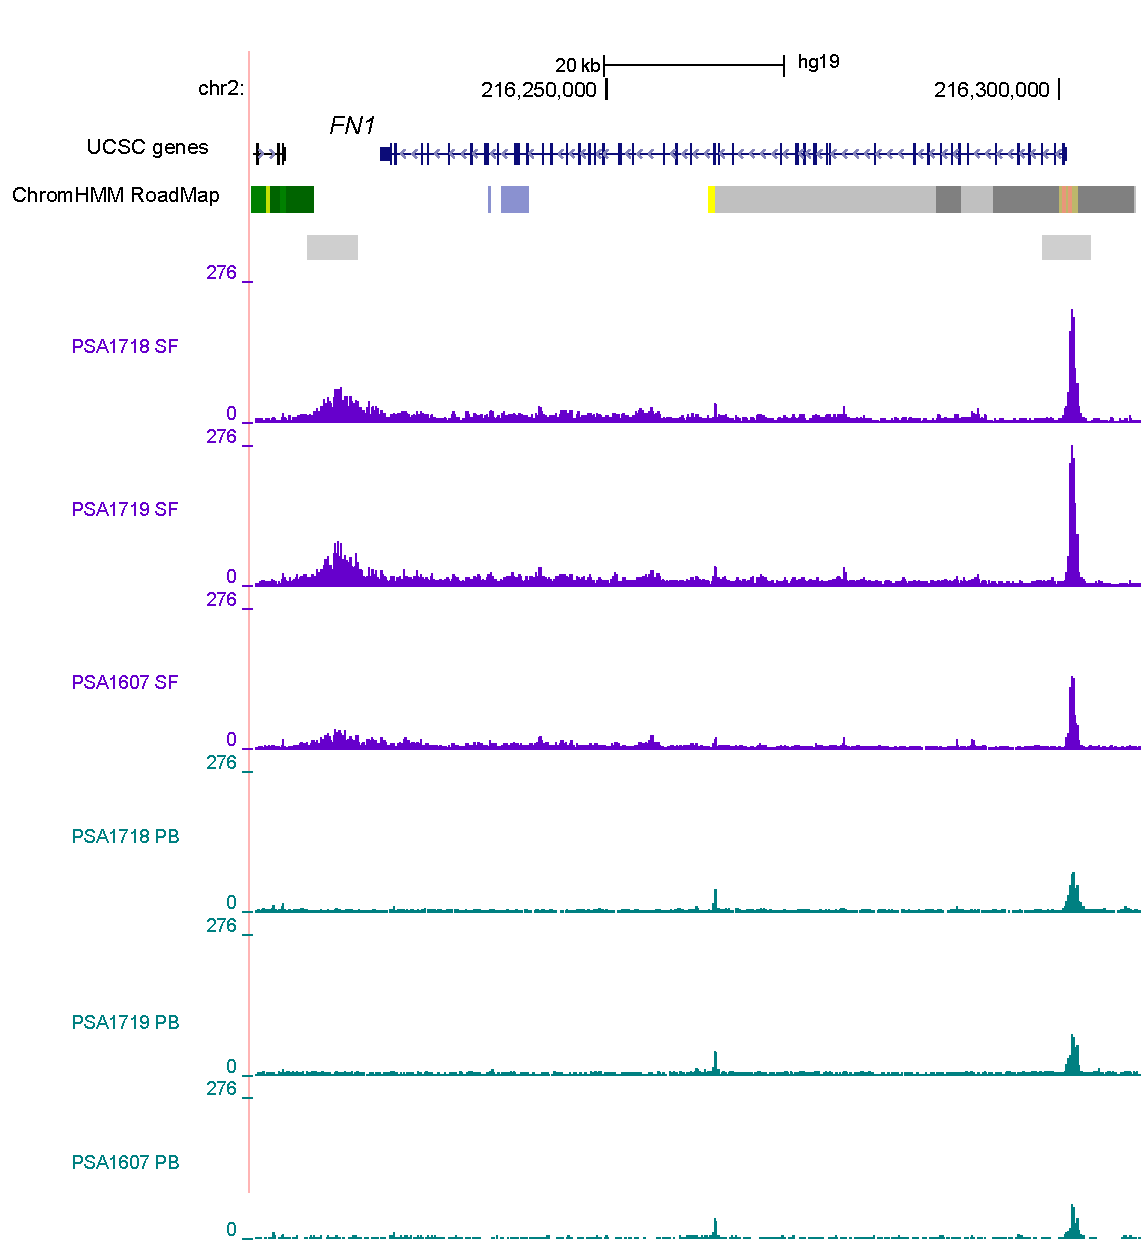
\includegraphics[width=0.6\textwidth]{./Results3/pdfs/PSA_CD14_ATAC_FN1_paired_gene_expression}
\caption[Chromatin accessibility landscape at the \textit{FN1} gene in CD14$^+$ monocytes isolated from SF and PB.]{\textbf{Chromatin accessibility at the \textit{FN1} gene in CD14$^+$ monocytes isolated from SF and PB.} xxxx }
\label{figure:PSA_CD14_ATAC_FN1}
\end{figure}

\subsubsection{Pathway enrichment and network analysis highlights the role of synovial CD14$^+$ monocytes in cytokine and chemokine production}
%Describe pathway analysis results and curate the pathway of interest
To identify relevant pathways amongst the modulated genes between SF and PB, enrichment analysis was performed for each individual cell type. Up-regulated and down-regulated genes showing abs mean FC $>$1.5 and pval$<$0.05 were used as input for the enrichment analysis. Interestingly, the modulated genes between SF and PB in CD14$^+$ monocytes were enriched for chemokine, NOD-like signalling and TLR signalling pathways (Table \ref{table:PSA_PCR_array_pathway_analysis}). All three pathways are involved in the activation of cytokines and chemokines gene expression, leading to T cell recruitment and inflammatory response. 

The TLR signalling pathways enrichment involved the \textit{FN1} (previously mentioned) and \textit{SPP1}, two of the top three most differentially expressed genes reported by Dolcino and colleagues in a study comparing synovial biopsies between healthy and PsA individuals \parencite{Dolcino2015} (Table \ref{table:PSA_PCR_array_pathway_analysis}). Together with \textit{FN1}, \textit{SPP1} was also one of the genes highly up-regulated (mean FC$>$16) in the three cell types (Figure \ref{figure:PSA_PCR_array_5pcnt_heatmap} orange box), showing the greatest FC in monocytes (Figure \ref{figure:PSA_PCR_array_vulcano_plots} a). Moreover, some of the genes driving enrichment, such as \textit{CCL5} and \textit{NFKB}, were also shared across the three pathways of interest. Others genes, including \textit{TNF}, \tetxit{IRF7} and \textit{MYD88}, highlighted the cross-link between the NOD-like and the TLR signalling pathways. 

Accordingly, the enrichment of SF open DARs in CD14$^+$ monocytes for the NF$\kappa$B pathway is closely related to the enrichment for TLR and NOD-like signalling pathways at the transcriptomic level (Figure \ref{figure:PSA_ATAC_pathway_analysis_all_DOC} a). Both, TLR and NOD-like pathways lead to the activation of the NF$\kappa$B TF, which induces transcriptional activation of pro-inflammatory cytokines, further supported by the enrichment of SF open DARs for IL-2, IL-3, IL-5 and GM-CSF pathways (Figure \ref{figure:PSA_ATAC_pathway_analysis_all_DOC} a). Moreover, the pivotal role of NF$\kappa$B in the immune transcriptional profile of SF CD14$^+$ monocytes  is additionally sustained at the chromatin accessibility level by the enrichment of SF accessible chromatin sites for this TF (Figure \ref{figure:PSA_TFBS}).  

The enrichment for the chemokine pathway in CD14$^+$ monocytes (Table \ref{table:PSA_PCR_array_pathway_analysis}) included modulated genes highly up-regulated (mean FC$>$16) in SF compared to PB (e.g \textit{CCL18} and \textit{CCL2}) for all three cell types (Figure \ref{figure:PSA_PCR_array_5pcnt_heatmap} orange box) as well as genes only consistently modulated between SF and PB in CD14$^+$ monocytes (e.g \textit{CCL28}, Figure \ref{figure:fig:PSA_PCR_array_5pcnt_heatmap} green box). The chemokine pathway includes production of chemotractant molecules involved in the recruitment of leukocytes to the site of inflammation and reactive oxygen species (ROS) through Ca$^2$$^+$ mobilisation, a pathway that has previously presented to be enriched in SF open DARs in CD14$^+$ monocytes (Figure \ref{figure:PSA_ATAC_pathway_analysis_all_DOC} a).

At the transcriptional level, significantly modulated genes between SF and PB in mCD4$^+$ T cells were enriched for the IL-10 signalling pathway (Table \ref{table:PSA_PCR_array_pathway_analysis}), in lines with the enrichment for IL signalling of open chromatin in SF cells (Figure \ref{figure:PSA_ATAC_pathway_analysis_all_DOC} b). % Add reference to this pathway in disease


\begin{landscape}
\begin{center}
\begin{longtable}[ht]{c c c }
\caption[Pathway enrichment analysis for the modulated genes between SF and PB in CD14$^+$ and mCD4$^+$.]{\textbf{Pathway enrichment analysis for the modulated genes between SF and PB in CD14$^+$ and mCD4$^+$.} The analysis was performed using only those genes showing pval$<$0.05 and mean FC$>$1.5. Reported enriched pathways were significant at an FDR $<$0.05.}
\\
\label{table:PSA_PCR_array_pathway_analysis} \\
\toprule
\textbf{Cell type} & \textbf{Pathway} & \textbf{Genes} \\						
\midrule
\midrule
\textbf{CD14$^+$} & Chemokine signalling & \textit{CCL17}, \textit{CCL18}, \textit{CCL2}, \textit{CCL28}, \textit{CCL5}, \textit{CCL7}, \textit{CCR1}, \textit{CCR5},\textit{CXCL10} \\  
									&                             & \textit{CXCL12}, \textit{CXCL16}, \textit{CXCL5}, \textit{CXCL9}, \textit{NFKB1}, \textit{PPBP}, \textit{PF4V1}, \textit{STAT3}, \textit{XCR1}\\
									
									& NOD-like receptor signalling & \textit{CCL2}, \textit{CCL5}, \textit{IFNAR1}, \textit{IL18}, \textit{IRF7}, \textit{MEFV}, \textit{MYD88}, \textit{NFKB1}, \\
									&                                         & \textit{NAMPT}, \textit{TNF} \\

									& TLR signalling   & \textit{CCL5}, \textit{CXCL10}, \textit{CXCL9}, \textit{IFNAR1}, \textit{IRF7}, \textit{MYD88}, \textit{NFKB1}, \textit{SPP1},\textit{FOS},\\ 
									&                                         & \textit{TLR1}, \textit{TLR2}, \textit{TLR8}, \textit{TNF}\\

\midrule
\textbf{mCD4$^+$} & IL-10 signaling & \textit{CCL3}, \textit{CCL4}, \textit{CCL5}, \textit{CCR1}, \textit{CCR2}, \textit{CSF1}, \textit{CSF3}, \textit{IL10RA}, \\
									&									& \textit{IL1R1}, \textit{IL1R2}\\
\bottomrule
\medskip
\end{longtable}
\end{center}
\end{landscape}

In addition to pathway enrichment, network analysis was performed to understand the interaction and relationship of the genes with modulated expression between SF and PB. A gene subnetwork was identified from the STRING functional interaction database using as input all the genes from the qPCR array (regardless significant modulation based on pval$<$0.05) and ranking them based on the best pval across the three analysed cell types. The identified subnetwork predominantly included significant modulated genes between SF and PB in at least one of the cell types. Amongst the most interesting nodes was the single Ig and Toll-interleukine domain containing gene (\textit{SIGIRR}), which is a negative regulator of the TLR signalling pathway (Figure \ref{figure:PSA_PCR_network_analysis}). \textit{SIGIRR} was significantly down-regulated in SF CD14$^+$ monocytes only and it is consistent with the significant up-regulation (pval<0.05) of the \textit{TLR1}, \textit{TLR2}, \textit{MYD88} genes in SF as well as the enrichment for the TLR pathway in this cell type (Figure \ref{figure:PSA_PCR_array_5pcnt_heatmap} and \ref{table:PSA_PCR_array_pathway_analysis}). Moreover, the significant up-regulation of \textit{NFKB} and \textit{TNF} in the SF CD14$^+$ monocytes appeared as a downstream result of the functional connection with TLR pathway members such as \textit{MyD88}, previously mentioned . Conversely, in mCD4$^+$ and mCD8$^+$ the modulation of these members did not appear to be significant between SF and PB; however, in mCD8$^+$, \textit{TNF} expression is also significantly up-regulated in the synovium compared to PB. 

Another interesting part of the network is the connection of the TLR pathway and the chemokine production through \textit{NF$\kappa$B}, \textit{TNF} and \textit{CCL2} (Figure \ref{figure:PSA_PCR_network_analysis}). \textit{CCL2} is connected to \textit{CXCL10} and subsequently with \textit{CCL18} and \textit{CCR5}, all chemokines regulating migration and infiltration of monocytes and memory T cells at the sites of inflammation. This network analysis also highlighted relationship between \textit{IL7R} and \textit{IL2RG} coding for the two chains of the IL-7R. Interestingly, these two nodes were only significantly up-regulated in SF CD14$^+$ monocytes when compared to PB, supporting the novel cell and context specific role of IL-7R and IL-7R polymorphism under inflammatory conditions in CD14$^+$ monocytes\parencite{Al-Mossawi2018}.

% I could also talk about the FOS, PROK2 and PTGS2

\begin{figure}[htbp]
\centering
\includegraphics[width=\textwidth]{./Results3/pdfs/PSA_PCR_array_network_analysis}
\caption[Protein network analysis based on the immune qPCR array expression data.]{\textbf{Protein network analysis based on the immune qPCR array expression data.} xxxx }
\label{figure:PSA_PCR_network_analysis}
\end{figure}

Overall, the integration of the chromatin accessibility and immune transcriptional data reinforced a relevant role of synovial CD14$^+$ monocytes in the production of cytokines and chemokines, likely leading to activation of the innate immune response and the recruitment of T cells to this site of inflammation. 



\subsubsection{Tissue and disease specificity in gene expression modulation and relevant biological pathways}

In order to better understand the disease and tissue specificity of the prior transcriptomic results, gene expression was analysed in CD14$^+$ monocytes, mCD4$^+$ and mCD8$^+$ isolated from PB in three healthy controls using the same qPCR array. In each of the cell types, the FC in was calculated for the mean PB expression across the three PsA patients compared to the mean expression of the three healthy controls (as detailed in Chapter \ref{ch:Mat}). Similar to the previous analysis, pvals for the FC significance were calculated for each particular genes. Integration of the previous results of modulated gene expression between SF and PB in PsA (see Immune-relevant gene expression by qPCR) with this analysis allowed the identification of three group of genes (Figure \ref{figure:PSA_PCR_array_HC_FC_correlation}). First, the genes only significantly modulated (based on pval and FC threshold criteria) in PB between controls and PsA were designated as systemic genes (Figure \ref{figure:PSA_PCR_array_HC_FC_correlation} green dots). Those genes were not significantly modulated in the prior analysis comparing SF versus PB within PsA patients and could then be considered as the circulating disease "footprint". In this respect, CD14$^+$ monocytes was the cell type with lower number of systemic modulated genes (14), compared to mCD8$^+$ (23) and mCD4$^+$ (42) (Figure \ref{figure:PSA_PCR_array_HC_FC_correlation}a, b and c). 


\begin{figure}[htbp]
\centering
\begin{subfigure}{0.6\textwidth}
\centering
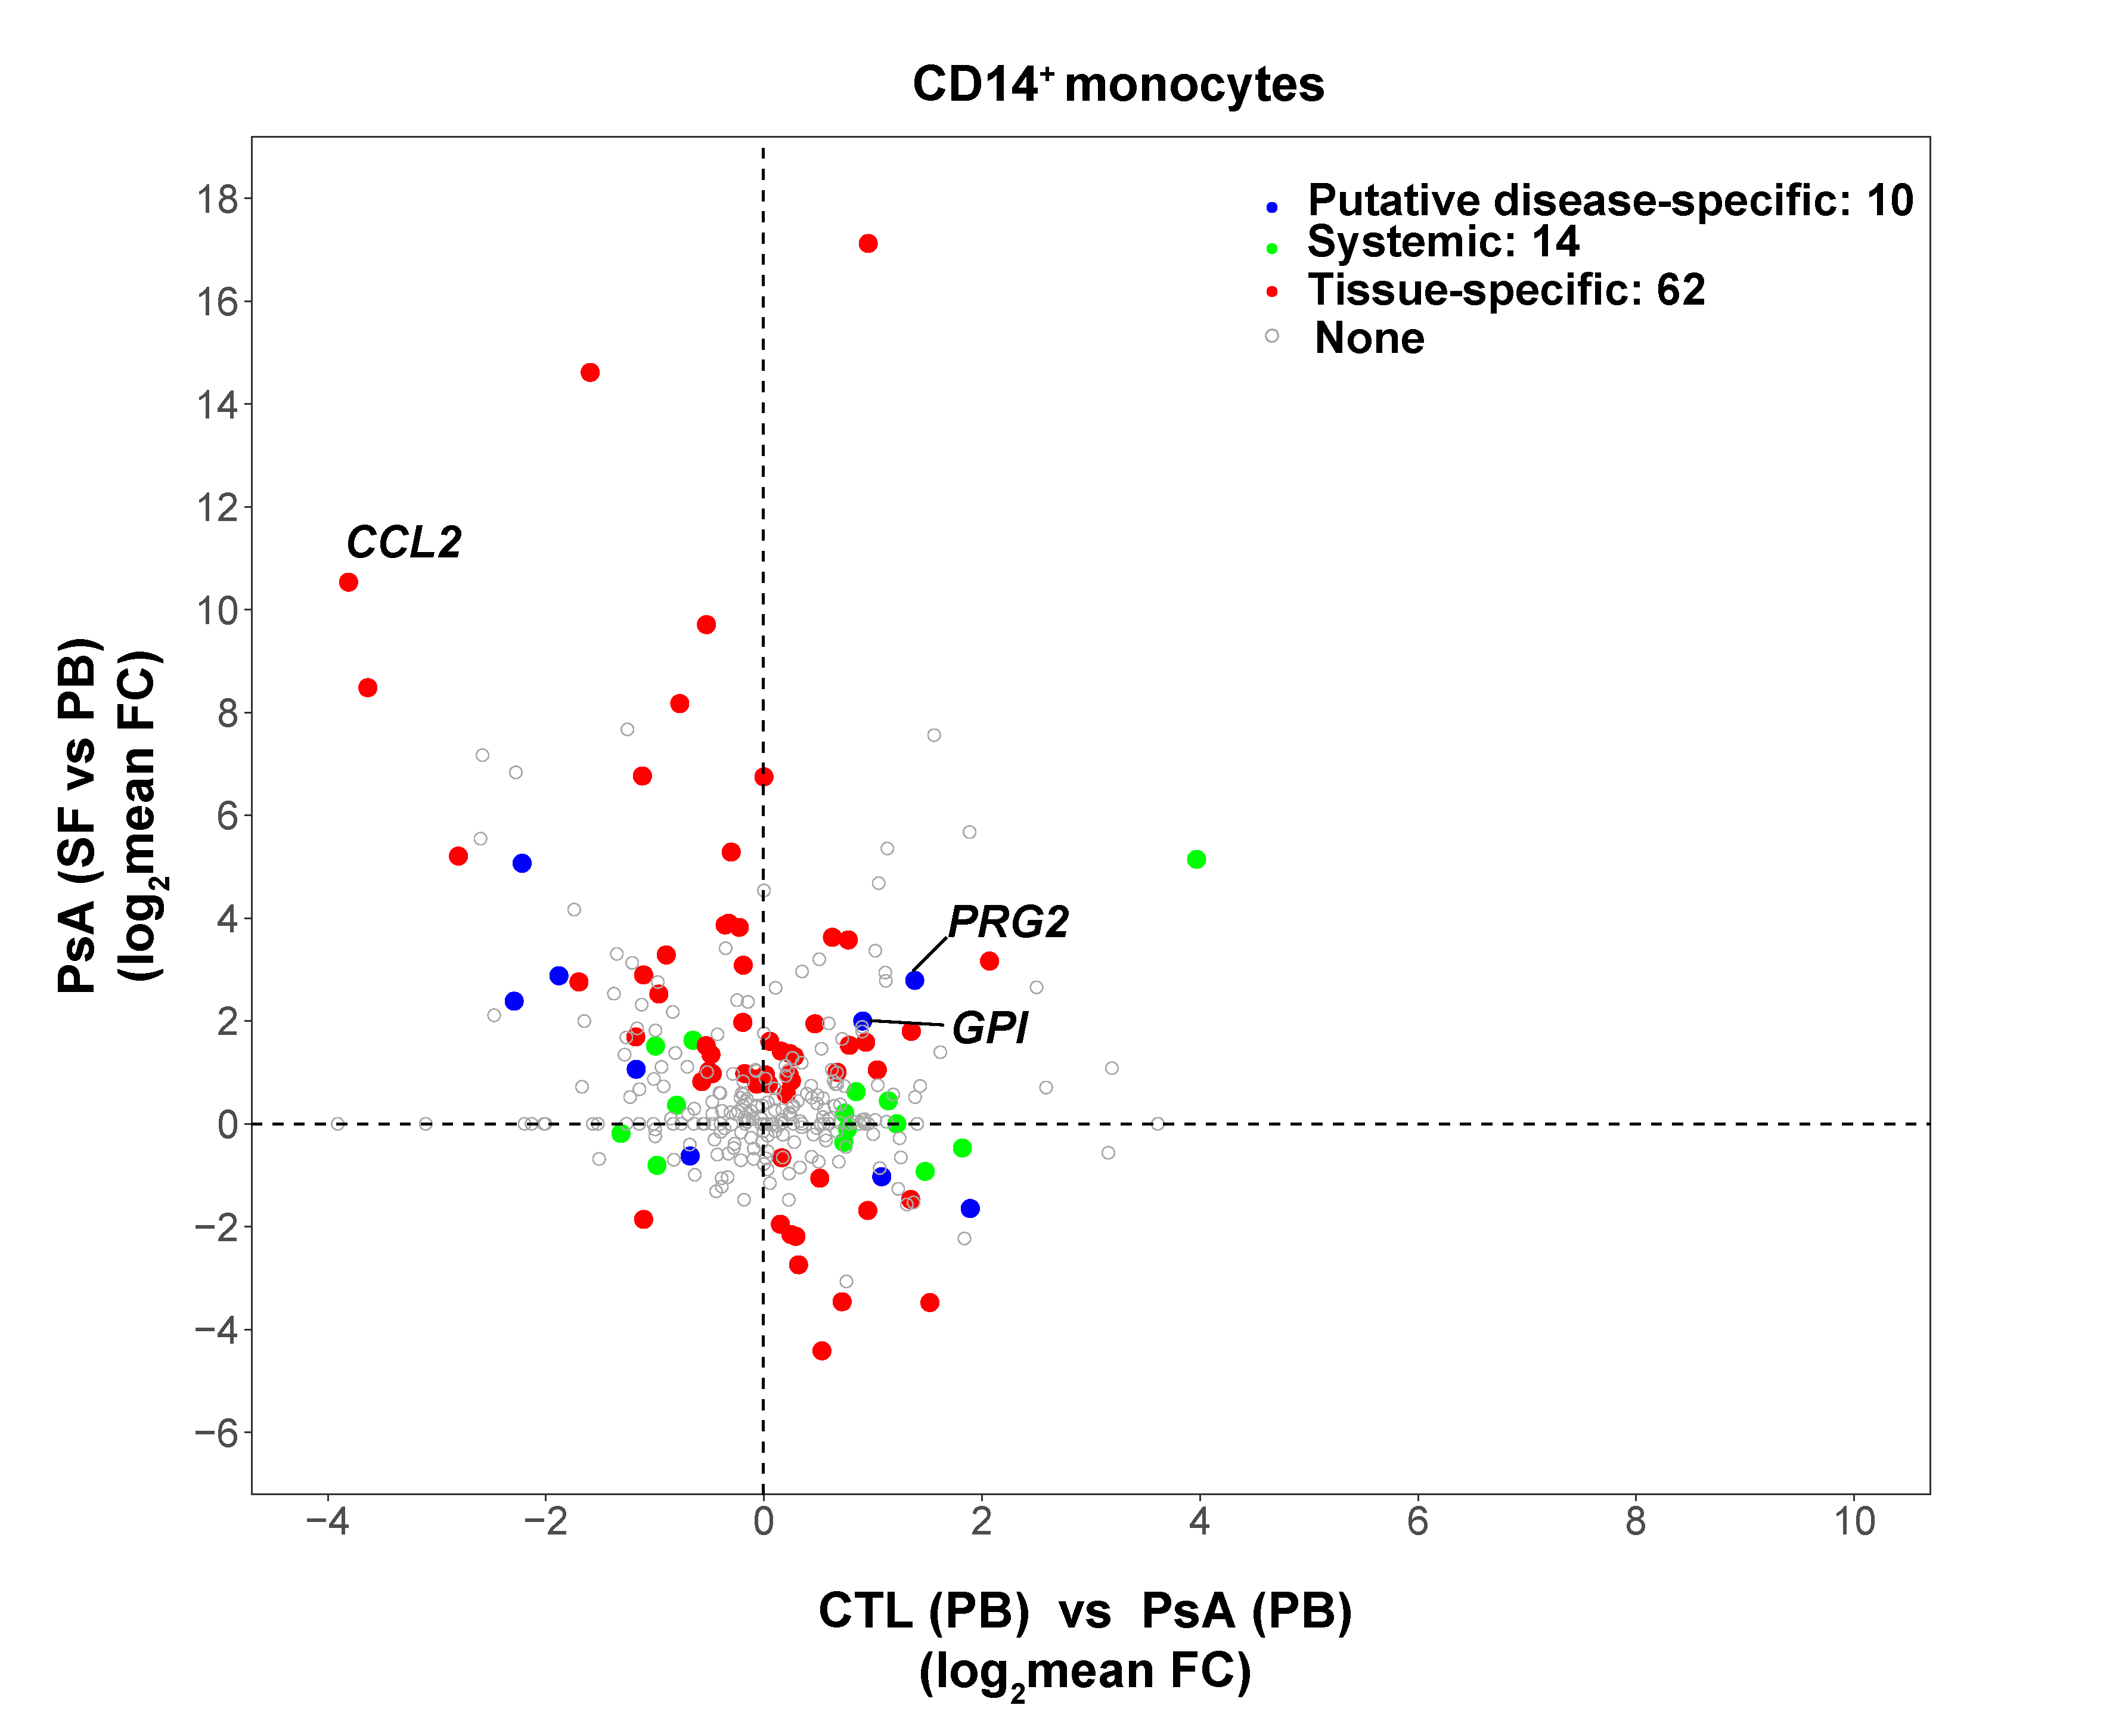
\includegraphics[width=\textwidth]{./Results3/pdfs/PSA_array_correlation_CD14_FC_HVPsA_vs_SFPBPsA_t}
\caption{\textbf{}}
% The percentage sign indicated that the other subfig goes side by side
\end{subfigure} \\
\begin{subfigure}{0.6\textwidth}
\centering
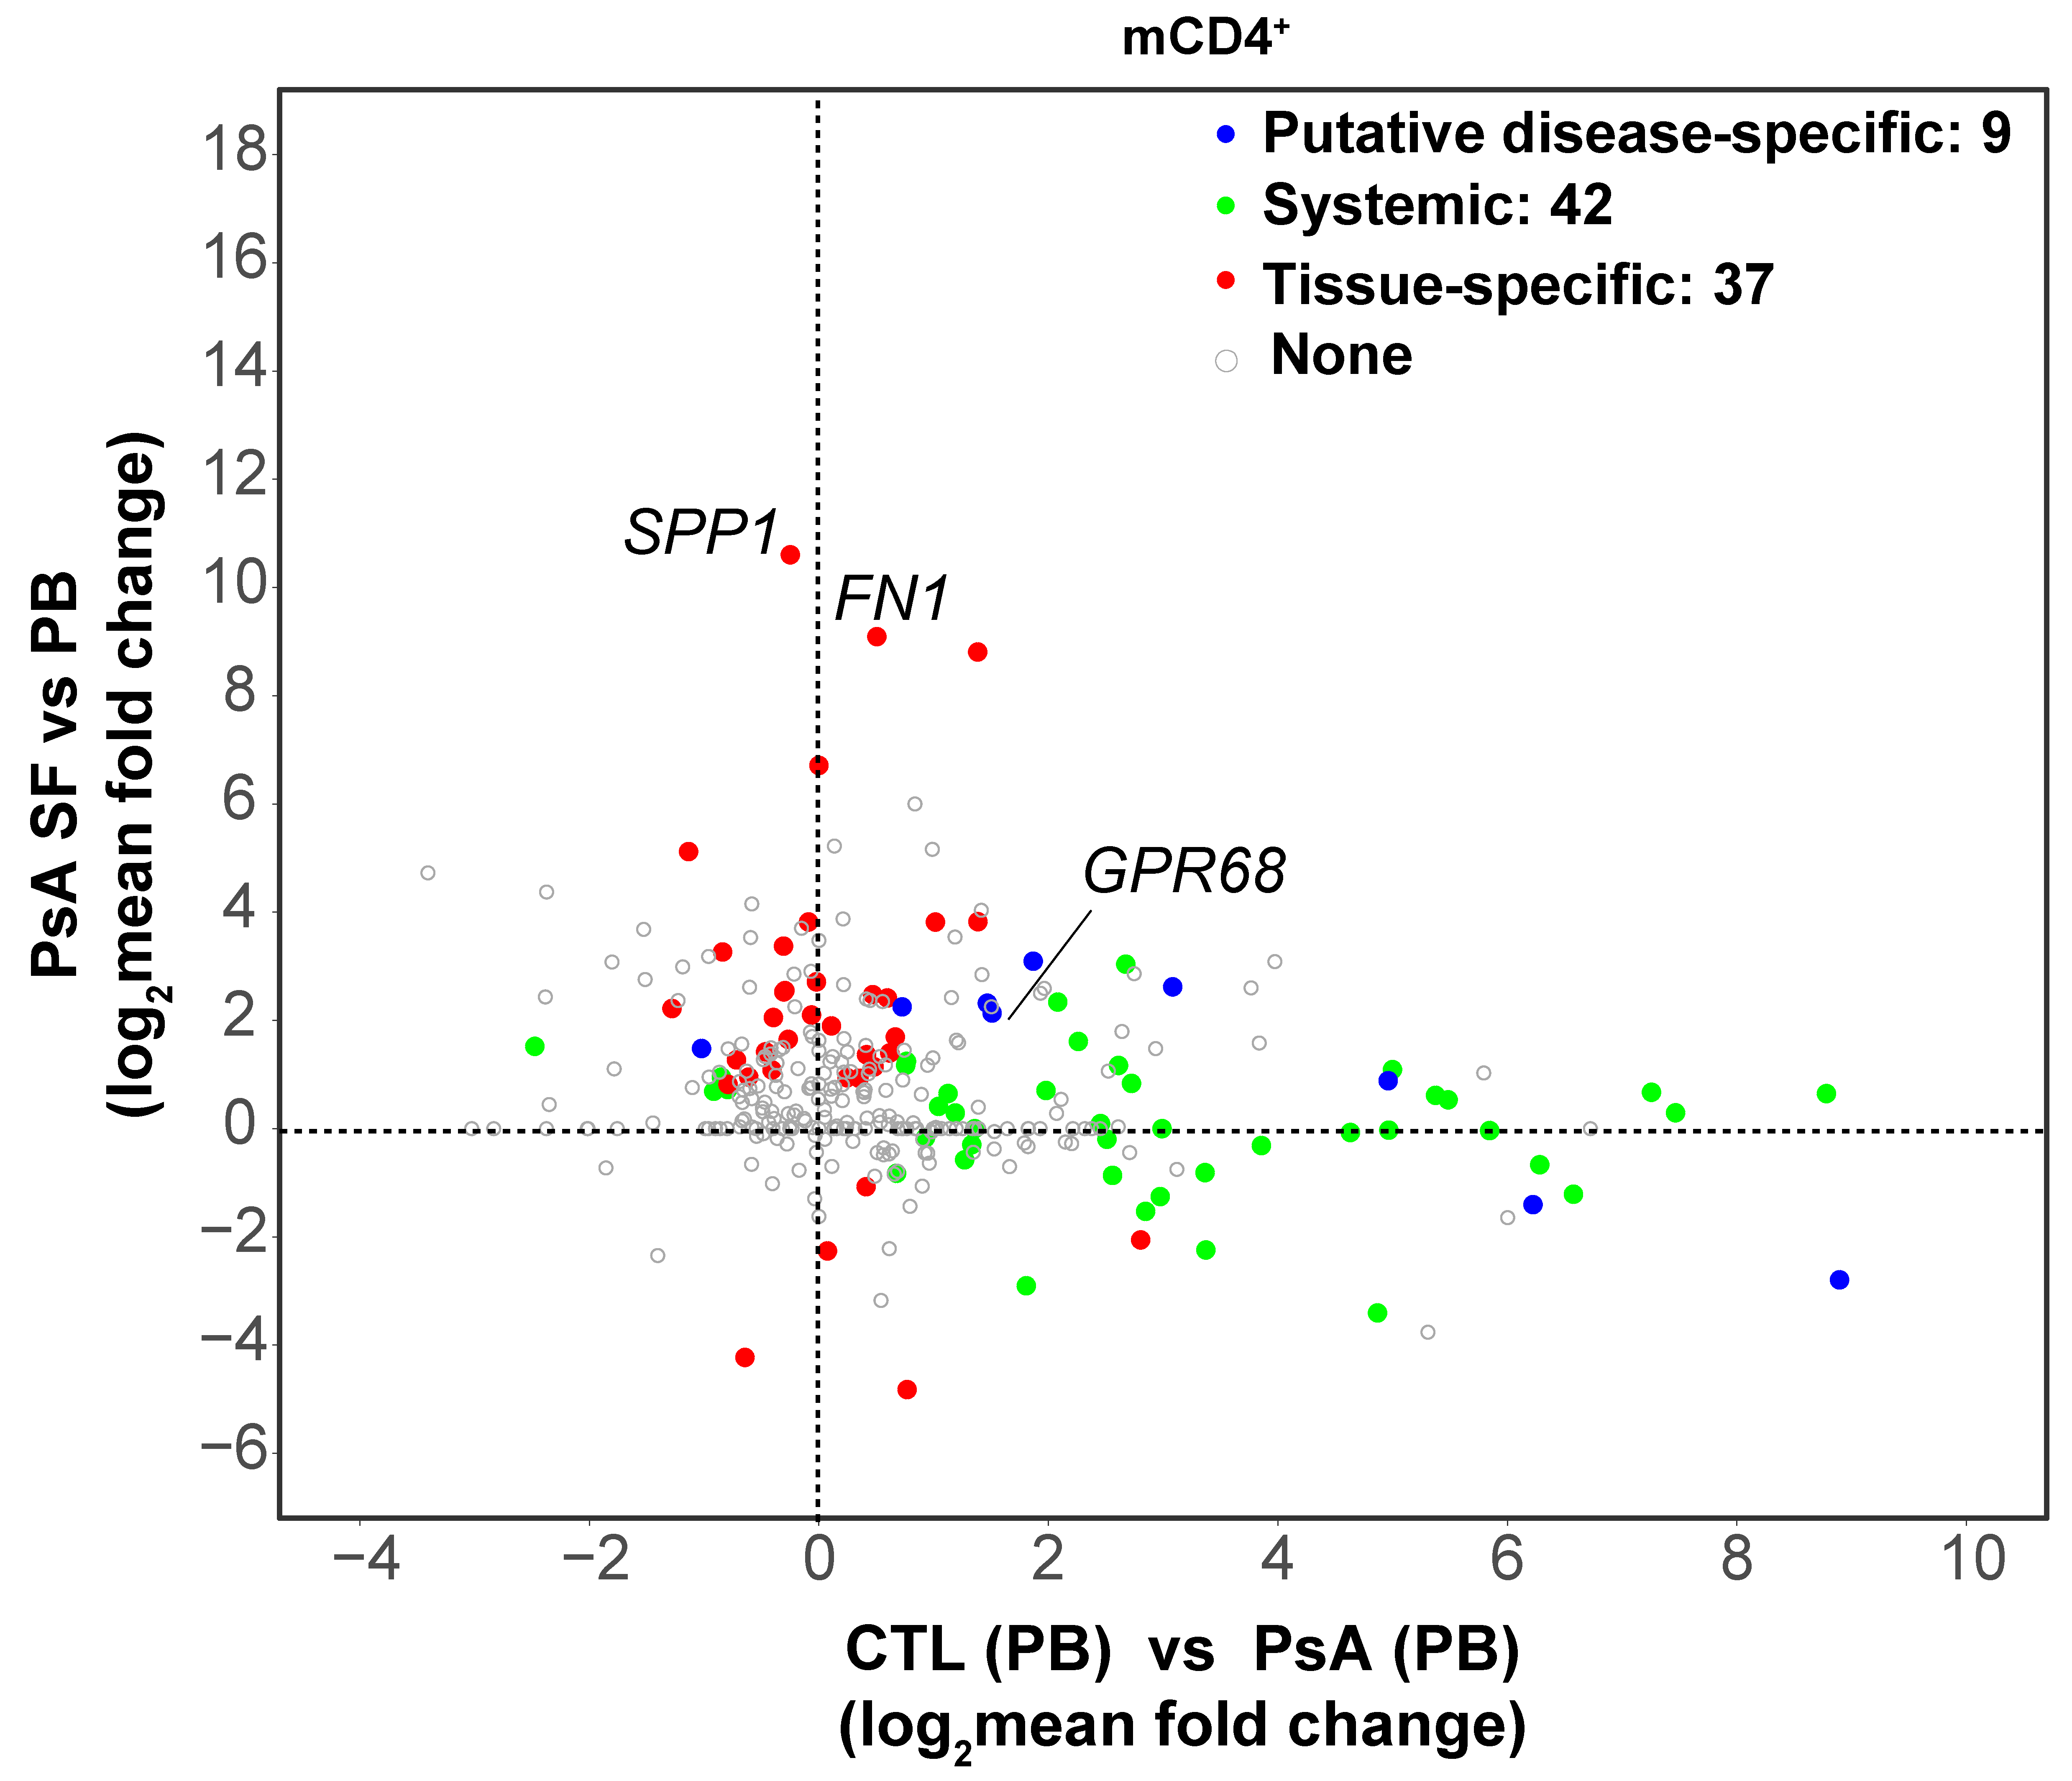
\includegraphics[width=\textwidth]{./Results3/pdfs/PSA_array_correlation_CD4_FC_HVPsA_vs_SFPBPsA}
\caption{\textbf{}}
\end{subfigure} %
\begin{subfigure}{0.6\textwidth}
\centering
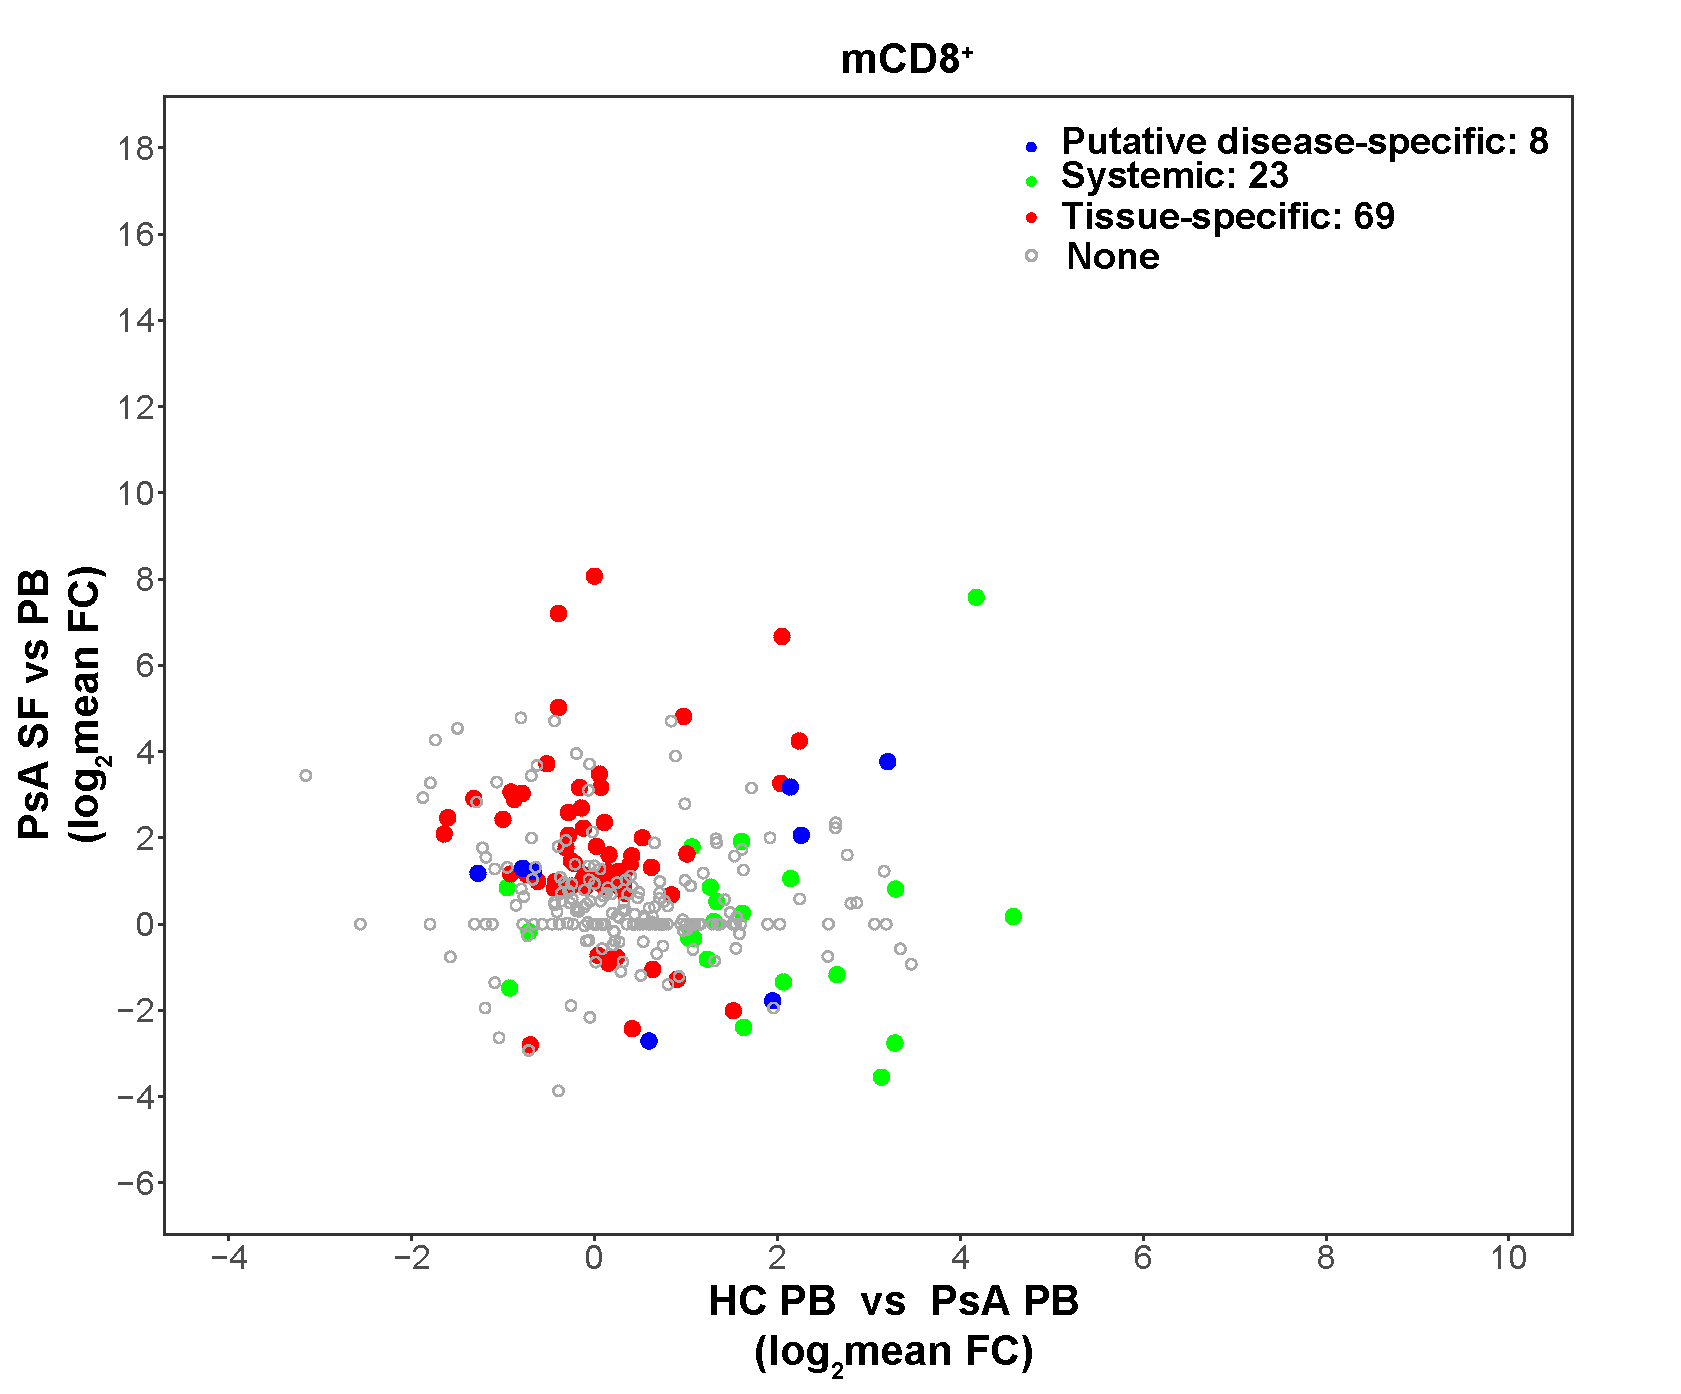
\includegraphics[width=\textwidth]{./Results3/pdfs/PSA_array_correlation_CD8_FC_HVPsA_vs_SFPBPsA}
\caption{\textbf{}}
\end{subfigure}
\caption[Expression changes in immune-relevant genes between SF and PB in CD14$^+$ monocytes, mCD4$^+$ and mCD4$^+$ cells.]{\textbf{Expression changes in immune-relevant genes between SF and PB in CD14$^+$ monocytes, mCD4$^+$ and mCD4$^+$ cells.}}
\label{figure:PSA_PCR_array_HC_FC_correlation}
\end{figure} 

A second group of genes were designated as tissue-specific, since they were significantly modulated between SF and PB in PsA patients but did not show significant changes between controls and PsA at the circulating level (Figure \ref{figure:PSA_PCR_array_HC_FC_correlation} red dots). Interestingly, in CD14$^+$ monocytes the tissue specific modulated genes considerably outnumbered the systemic ones (62 versus 14), showing a more pronounced change in the expression profile of immune genes across patients' tissues than between healthy and diseased PB (Figure \ref{figure:PSA_PCR_array_HC_FC_correlation} a red dots). For example, the aforementioned \textit{NFKB} and \textit{MYD88}, \textit{TLR2} genes were only up-regulated in PsA SF CD14$^+$ monocytes and their expression was not significantly modulated between healthy controls and PsA circulating CD14$^+$ monocytes.  Similarly to CD14$^+$ monocytes, mCD8$^+$ cells also presented greater disease tissue-specific modulation than genes differentially expressed when compared to controls in PB (Figure \ref{figure:PSA_PCR_array_HC_FC_correlation} c red dots).  
%Some more biology?
% talk about limitations in acknowledging these genes as dissease-tissue specific due to the fact that we don't know if they also change between PB and Sf in HV

The third category comprised genes significantly modulated for each cell type between controls and PsA patients in PB as well as between SF and PB in PsA patients. These genes defined as putative disease-specific genes presented similar numbers across CD14$^+$ monocytes, mCD4$^+$ and mCD8$^+$ (10, 9 and 8, respectively) (Figure \ref{figure:PSA_PCR_array_HC_FC_correlation} blue dots in a, b and c). In CD14$^+$ monocytes two of those genes, \textit{GPI} and \textit{PRG2}, were up-regulated in both comparisons, with further exacerbation in SF (Figure \ref{figure:PSA_PCR_array_HC_FC_correlation} a). Evidence of the glucose-6-phosphate isomerase \textit{GPI} up-regulation in disease has been found in RA synovial fibroblasts and linked to increased levels of TNF-$\alpha$ and IL-1$\beta$ in the synovium \parencite{Zhong2015}. % GPI fibroblasts https://www.ncbi.nlm.nih.gov/pmc/articles/PMC4422595/
Another example of exacerbated up-regulation in SF was the expression of \textit{GPR68} in mCD4$^+$. This gene was up-regulated in PsA PB mCD4$^+$ when compared to the control counterparts and further up-regulated in SF when compared to PB in PsA individuals (Figure \ref{figure:PSA_PCR_array_HC_FC_correlation} b). \textit{GPR68} is a G protein-coupled receptor, expressed in T cells, amongst other cells, that undergoes activation through pH acidification, characteristic of synovial tissues under inflammation \parencite{Biniecka2016}. \textit{GPR68} activation leads to an increase of Ca$^2$$^+$ levels and subsequent activation of immune-related pathways \parencite{Saxena2011}. \textit{GPR68} was also up-regulated in SF compared to PB in mCD8$^+$ cells, reinforcing the relevance of this gene in the synovial pathophysiological aspect of PsA.Amongst the genes presenting an opposite behaviour is the epidermal growth factor-like amphiregulin (\textit{AREG}), which in mCD8$^+$ is significantly up-regulated in PsA PB compared to the controls but is down-regulated in PsA individuals when comparing SF versus PB (Figure \ref{figure:PSA_PCR_array_HC_FC_correlation} c). \textit{AREG} defficiency in mouse models have shown an impaired immunosupressive response by Treg cells \parencite{Zaiss2013}, which could be contributing to the exacerbated immune response in the synovium. 
% GPR68 https://ard.bmj.com/content/73/Suppl_2/511.2
%GPR68 Hypoxia Positively Regulates the Expression of pH-Sensing G-Protein–Coupled Receptor OGR1 (GPR68)
%talk about limitations of those genes to be identified as disease specific. This would need an additional comparison between HV SF and PsA SF to make sure that those genes are not modulated in SF of HV and therefore are a lanmark of disease in both tissues
Despite the interesting aforementioned findings, the identification of disease-specific and disease tissue-specific genes is clearly limited by the impossibility of obtaining healthy controls SF to include in the experimental design.

When performing pathway enrichment analysis using the significantly modulated genes between healthy controls and PsA patients PB in the qPCR array, only the Reactome immune system pathway appeared as significant for CD14$^+$ monocytes and mCD4$^+$ cells. This result reinforced the tissue-specificity of the pathways enriched for the modulated genes between SF and PB in CD14$^+$ monocytes PsA patients and clearly suggest a more pronounced inflammatory phenotype of the pathological CD14$^+$ monocytes in SF compared to PB.



\subsection{Characterisation of the CD14$^+$ monocyte heterogeneity in PsA using scRNA-seq}
According to the analysis of chromatin accessibility and immune-related gene expression in this pilot cohort, the CD14$^+$ monocytes appeared as the studied population showed the greatest changes in chromatin accessibility and the most reliable modulation of expression for pro-inflammatory chemokines and cytokines between PB and SF. Since monocytes are very plastic cells which differentiate into macrophages at the site of inflammation, exploring differences at the single-cell level and integrating chromatin accessibility and gene expression data could highlight subpopulations of particular interest and help to better understand the differences in the immune response between the blood and the inflamed tissue.


\subsubsection{scRNA-seq reveals two main subpopulations in SF and PB combined CD14$^+$ monocytes}
%Explain how I did the analysis
ScRNA-seq was performed in paired PBMCs and SFMCs isolated from three PsA patients (Table \ref{tab:PSA_datasets_per_sample}). scRNA-seq data from each of the PBMCs and SFMCs samples, were filtered as explained in \ref{ch:Mat} and CD14$^+$ monocytes were subset from the rest of the cells by expression of \textit{CD14} and \textit{LYZ}, the two of the most accurate expression markers defining this cell population (Figure \ref{figure:PsA_scRNAseq_SF_an_PB_monocytes_identification_from_bulk} a and b). Across all six samples (three SFMCs and three PBMCs), 2,459 cells were CD14$^+$ monocytes cells, representing approximately 17\% of the bulk SFMCs and PBMCs cells in line with the proportion of CD14$^+$ monocytes previously reported using mass cytometry cell surface markers (Figure \ref{figure:PsA_cell_composition}). The CD14$^+$ monocytes identified in each of the three PsA paired PBMCs-SFMCs samples were combined using CCA to correct for the batch effect intrinsic unavoidable patients' sample recruitment at different days and generation of SFMCs and PBMCs libraries separately. CCA alignament of the six CD14$^+$ monocytes populations was followed by conservative unpervised clustering (using resolution 0.1) and t-SNE visualisation. 

\bigskip
\begin{figure}[H]
\centering
\begin{subfigure}[b]{0.60\textwidth}
\centering 
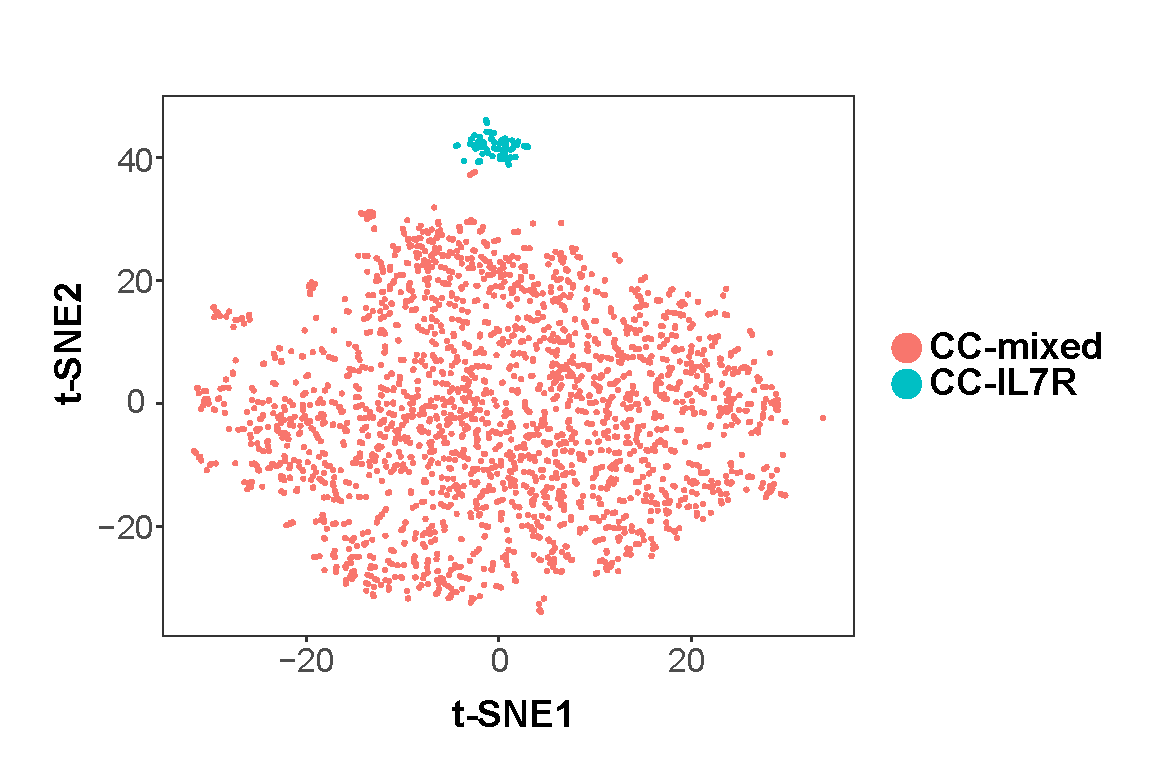
\includegraphics[width=\textwidth]{./Results3/pdfs/PSA_scRNAseq_tSNE_CC_mixed_and_IL7R}
\caption{}
\end{subfigure}
~
\begin{subfigure}[b]{0.75\textwidth} 
%the [b] prevents offset in subcaptions
\centering
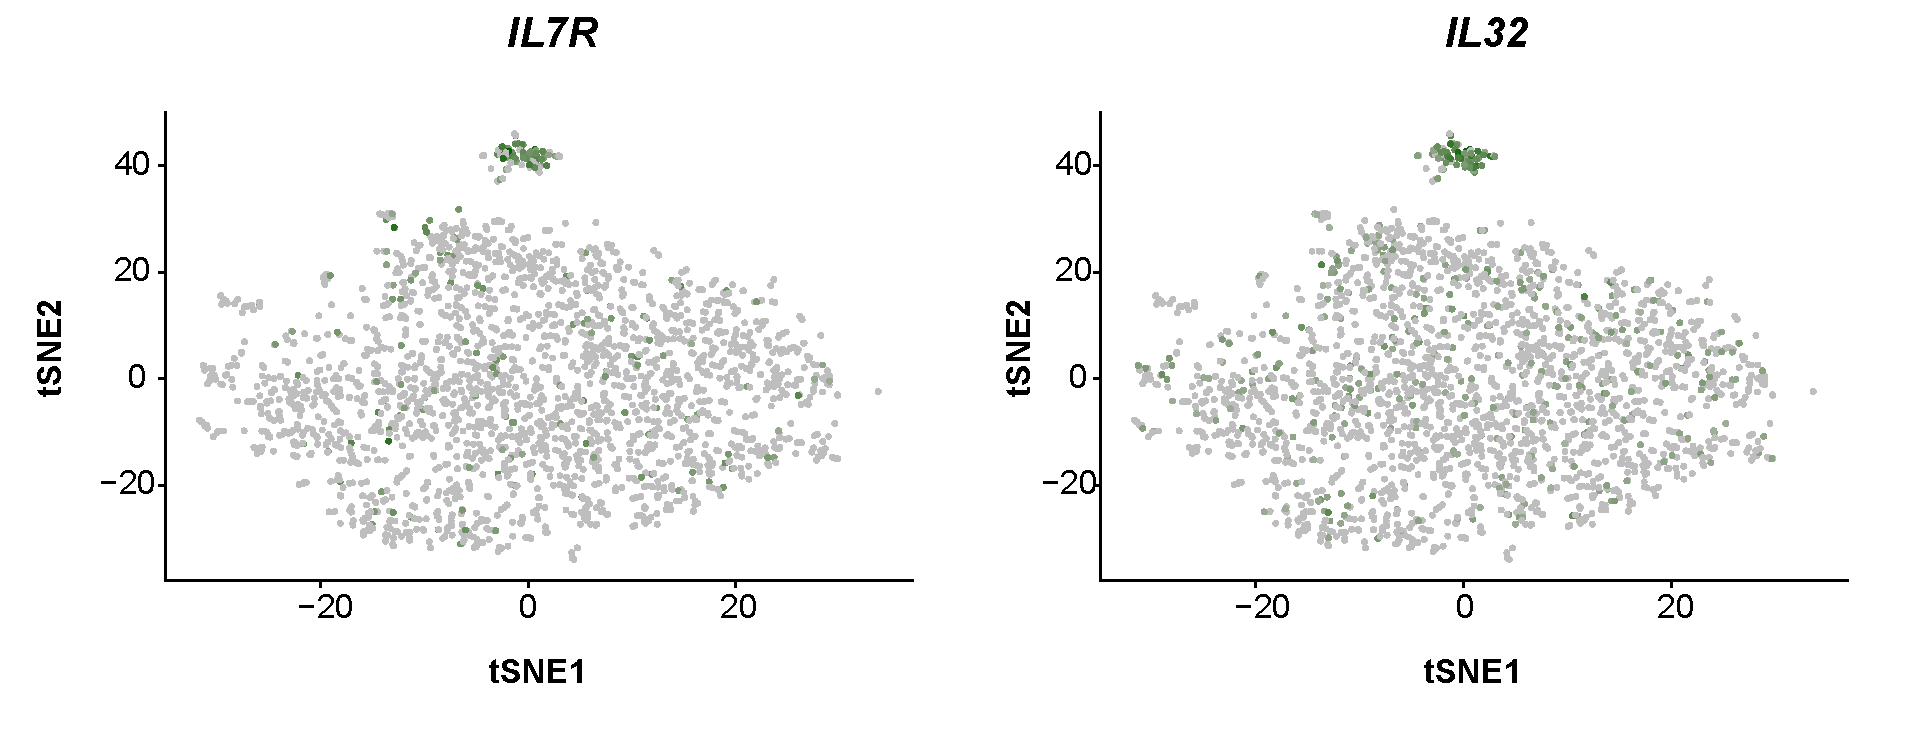
\includegraphics[width=\textwidth]{./Results3/pdfs/PSA_scRNAseq_CC_mixed_and_IL7R_overlay_markers}
\caption{}
\end{subfigure}
\caption[Identification of two main CD14$^+$ monocytes subpopulations in the SF and PB combined analysis]{\textbf{Identification of two main CD14$^+$ monocytes subpopulations in the SF and PB combined analysis.} a) Visualisation using tSNE dimensional reduction of the two cluster, CC-mixed and CC-IL7R, identified from the combined SF and PB CD14$+$ monocyte cells using a very conservative resolution for the unsupervised clustering analysis. b) Overlap of \tetxit{IL7R} and \textit{IL32} expression intensities by the CC-mixed and CC-IL7R CD14$+$ monocytes.}
\label{figure:PsA_scRNAseq_SF_an_PB_monocytes_identification_from_bulk}
\end{figure}

%Say that using a conservative approach to find cluster two main groups were identified: No IL7R vs IL7R
%Probably more heterogeneity could be found within the big cluster but given number of replicates and intensive analysis required to make sure clusters are estable we decided to only trust these two main groups
Using this conservative approach, two robust clusters were identified (Figure \ref{figure:PsA_scRNAseq_SF_an_PB_monocytes_identification_from_bulk} a). The smallest cluster, named a CC-IL7R, was characterised by the expression of \textit{IL7R}, \textit{IL32} and \textit{CCL5}, amongst others, and was formed by a total of 72 cells (43 from SF versus 29 from PB) (Figure \ref{figure:PSA_scRNAseq_CC_mixed_and_IL7R_overlay_markers} b and \ref{figure:PSA_scRNAseq_CC_mixed_and_IL7R_markers_heatmap}) (\parencite{Al-Mossawi2018}, in revision). The proportion of IL7R$^+$CD14$^+$ monocytes when compared to the total number CD14$^+$ monocytes was very similar in SF and PB (3 and 2.7\%, respectively) in this data. The largest cluster, named as CC-mixed, was formed by 2,387 (1,356 SF and 1,031 PB). CC-mixed was quite heterogeneous, without consistent expression pattern for those genes identified as cluster markers (Figure \ref{figure:PSA_scRNAseq_CC_mixed_and_IL7R_markers_heatmap}). Similar results were obtained when increasing the resolution parameter to identify additional clusters, failing to find consistency in the expression patters not even for the top genes defined as markers for the clusters (data not shown). Increasing cohort size and a more exhaustive analysis could be use to identify additional subpopulations within the CD14$^+$ monocytes from SF and PB in the CC-mixed cluster. For the scope of this project, downstream analysis, including DGE between the two tissues, was performed in the CC-mixed and CC-IL7R clusters identified by the most conservative approach.





\subsubsection{Differential gene expression between SF and PB CD14$^+$ monocytes in CC-mixed and CC-IL7R}
%DGE was performed between tissues within each cluster
DGE analysis was performed in order to explore the differences between SF and PB at a genome-wide level within each of these two main CD14$^+$ monocytes subpopulations. In the CC-mixed cluster, a total of 251 genes were differentially expressed at an FDR$<$0.01 and abs(FC)$>$1.5 in SF compared to PB, of which 149 and 102 presented up- and down-regulation, respectively (Figure \ref{figure:PsA_scRNAseq_vulcano_plots_mixed_and_IL7R_clusters} a). Differential analysis in the CC-IL7R revealed a total of 37 modulated genes, with the majority (35 out of 37) up-regulated in SF compared to PB (Figure \ref{figure:PsA_scRNAseq_vulcano_plots_mixed_and_IL7R_clusters} a). Due to the low number of cells in the CC-IL7R cluster and the small sample size (n=3), the differential analysis only identified as significantly differentially expressed (FDR$<$0.01) genes presenting abs(FC)$>$1.5. Of the 37 genes differentially expressed between the two tissues in the CC-IL7R cluster, 30 were shared with the CC-mixed cluster. The 7 distinctly modulated genes in the CC-IL7R cluster included \textit{CD44}, \textit{MT-CO2} or S-ribosomal protein (RPS) genes (\textit{RPS29} and \textit{RPS27}). \textit{CD44} is a receptor of the hialuronic acid and also osteopontin, the product from the aforementioned \textit{SPP1} gene, which acts as an immune modulator increasing chemotaxis, cell activation and cytokine production. Although \tetxit{SPP1} is the gene presenting the greatest up-regulation in SF when compared to PB in the two CD14$^+$ monocytes clusters (Figure \ref{figure:PsA_scRNAseq_vulcano_plots_mixed_and_IL7R_clusters} a and b), monocytes from the CC-IL7R subpopulation may be more responsive to this chemokine.


\bigskip
\begin{figure}[H]
\centering
\begin{subfigure}[b]{0.70\textwidth}
\centering 
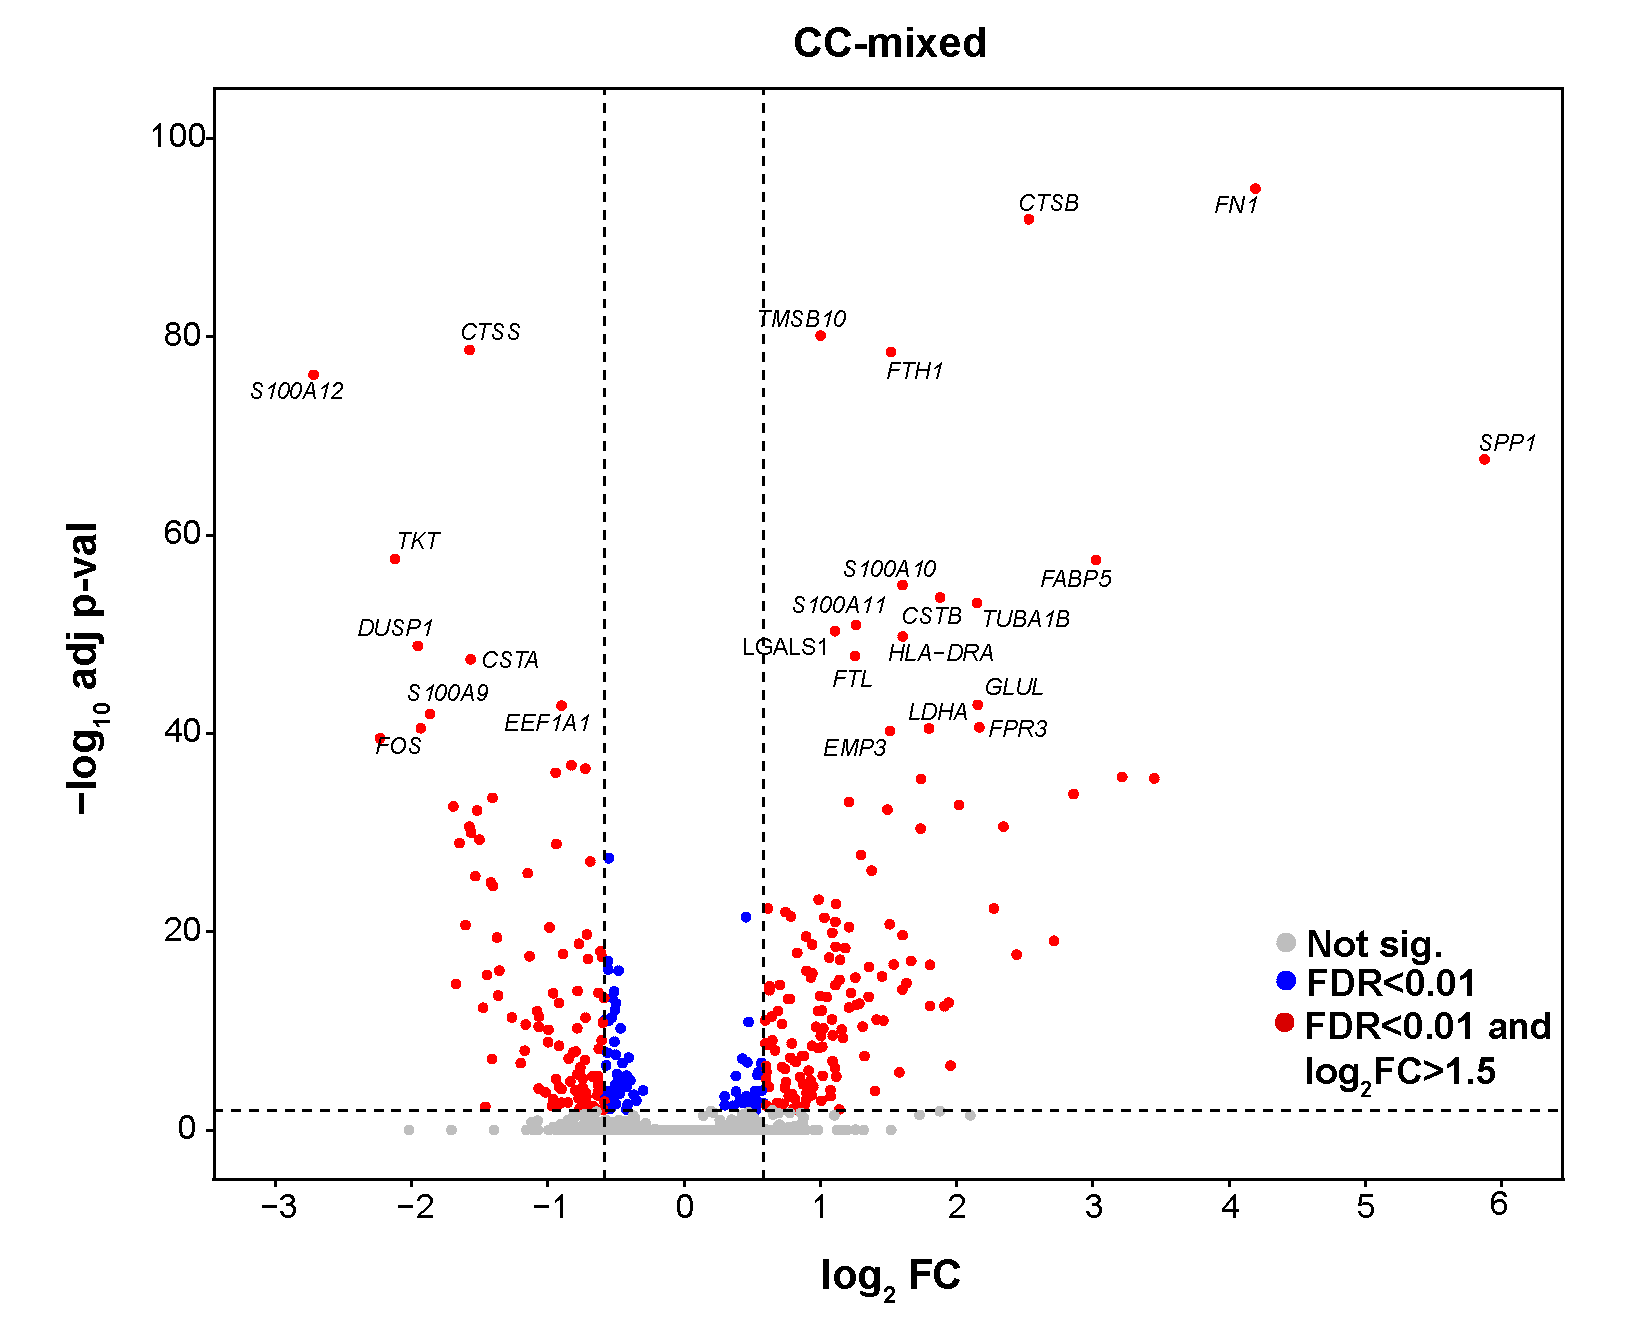
\includegraphics[width=\textwidth]{./Results3/pdfs/PSA_10X_all_combined_aligned_monocytes_DGE_SF_vs_PB_cluster_0_vulcano_plot}
\caption{}
\end{subfigure}
~
\begin{subfigure}[b]{0.70\textwidth} 
%the [b] prevents offset in subcaptions
\centering
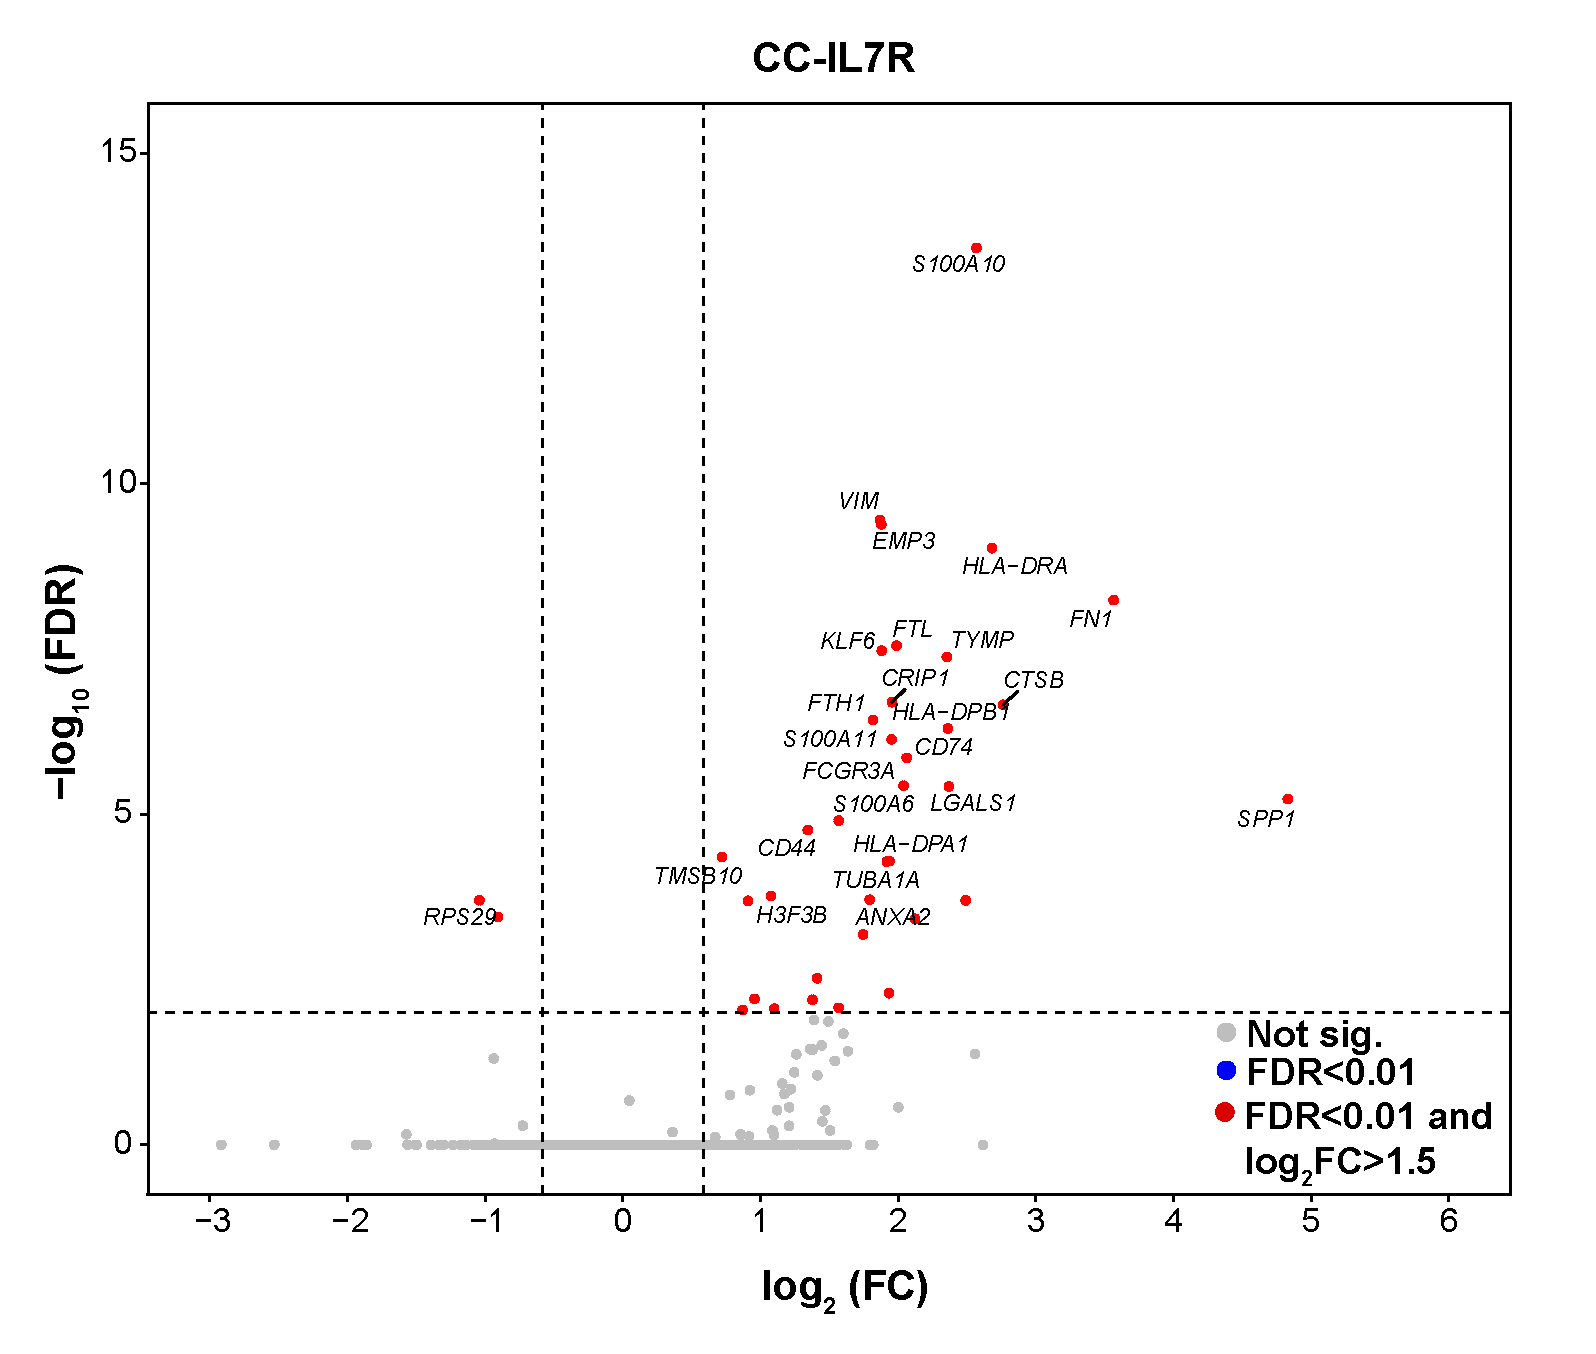
\includegraphics[width=\textwidth]{./Results3/pdfs/PSA_10X_all_combined_aligned_monocytes_DGE_SF_vs_PB_IL7R_vulcano_plot}
\caption{}
\end{subfigure}
\caption[Sc-RNA-seq differential gene expression results between SF and PB in the CC-mixed and CC-IL7R CD14$^+$ monocytes subpopulations.]{\textbf{Sc-RNA-seq differential gene expression results between SF and PB in the CC-mixed and CC-IL7R CD14$^+$ monocytes subpopulations.} xxxx}
\label{figure:PsA_scRNAseq_vulcano_plots_mixed_and_IL7R_clusters}
\end{figure}

% Pathway analysis
Pathway enrichment analysis was performed for the significantly DEGs between SF and PB in the CC-mixed and CC-IL7R subpopulations. The DEGs in the CC-mixed cluster were enriched for Ag processing and presentation pathway contributed by up-regulation expression in the SF of \textit{CD74} and genes from the \textit{HLA-D} family \parencite{Lamb1992} (Table \ref{tab:PSA_scRNAseq_CD14_DEGs_pathway_analysis} and \ref{tab:PSA_scRNAseq_CC_mixed_and_IL7R_additional_pathways}). Enrichment for IFN signalling was driven by the \textit{IFI6}, \textit{IFITM3}, \textit{LY6E}, \textit{ISG15} and the TF \textit{STAT1}, all of them up-regulated in SF when compared to BD CD14$^+$ monocytes. Interestingly, \textit{IFI6}, \textit{IFITM3}, \textit{LY6E} have been identified as markers of a subpopulation of CD14$^+$ monocytes for RA \parencite{Zhang2018}. Another relevant enriched pathway was the extracellular matrix and extracellular matrix-associated proteins which involves genes of the S100 family (including \textit{S100A8}, \textit{S100A9}, \textit{S100A10}, \textit{S100A11} and S100A12, that interact with the receptor for advance glycosylation end products (RAGE) and induce production of matrix-degrading enzymes involved in joint erosion and development of arthritis \parencite{Raghunatha2012}. Two genes of this family, \textit{S100A8} and \textit{S100A9} also appeared to be dysregulated in lesional skin compared to uninvolved in Chapter \ref{ch:Results2} and contributed in the significant enrichment for the IL-17 signalling pathway in inflamed skin. However, \textit{S100A8} and \textit{S100A9} were up-regulated in lesional skin whereas they appeared down-regulated in SF compared to PB. The phagosome and lysosome formation pathway also appeared to be more active in SF CD14$^+$ monocytes, where up-regulation of genes such as \textit{CTSL}, which is involved in protein degradation in lisosomes and phagocytosis of apoptotic cells. %Lastly, enrichment for cytokine signalling included, for example, the insulin receptor substrate\textit{IRS2} and up-regulation of the kinase \textit{MAP3K8} which activates MAPK and JNK kinase pathways (ref). 
The most functionally relevant significantly enriched pathways identified for DEGs in the CC-IL7R subpopulation were common to the ones found in the CC-mixed cluster (Table \ref{tab:PSA_scRNAseq_CD14_DEGs_pathway_analysis}).

Interestingly, the overlap of DEGs with the qPCR array was modest, particularly for the DEGs in the CC-IL7R. Amongst the 72 DEGs (pval<0.05)detected by qPCR between SF and PB in CD14$^+$ monocytes, only 13 and 4 genes were also differentially expressed (FDR$<$0.01 and no FC threshold) in the CC-mixed and CC-IL7R clusters, respectively (Figure \ref{figure:figure:PsA_scRNAseq_qPCR_ATAC_correlation} a). The genes which differential expression between SF and PB was reproducible included genes with the largest FCs in both assays, such as \textit{SSP1}, \textit{FN1}, \textit{OLR1} and \textit{S100A12}and the direction of change was consistent for all of them. %add something about cell type specificity
%Regarding the low number of qPCR DEGs between SF and PB in total CD14$^+$ monocytes reproduced by the scRNA-seq in any of the two main clusters identified could be explained by the differences in the cell sorting (FACS versus \textit{in silico} expression markers), the low number of replicates for each assay as well as different sensitivity of the two technologies.   
   
\bigskip
\begin{figure}[H]
\centering
\begin{subfigure}[b]{0.50\textwidth}
\centering 
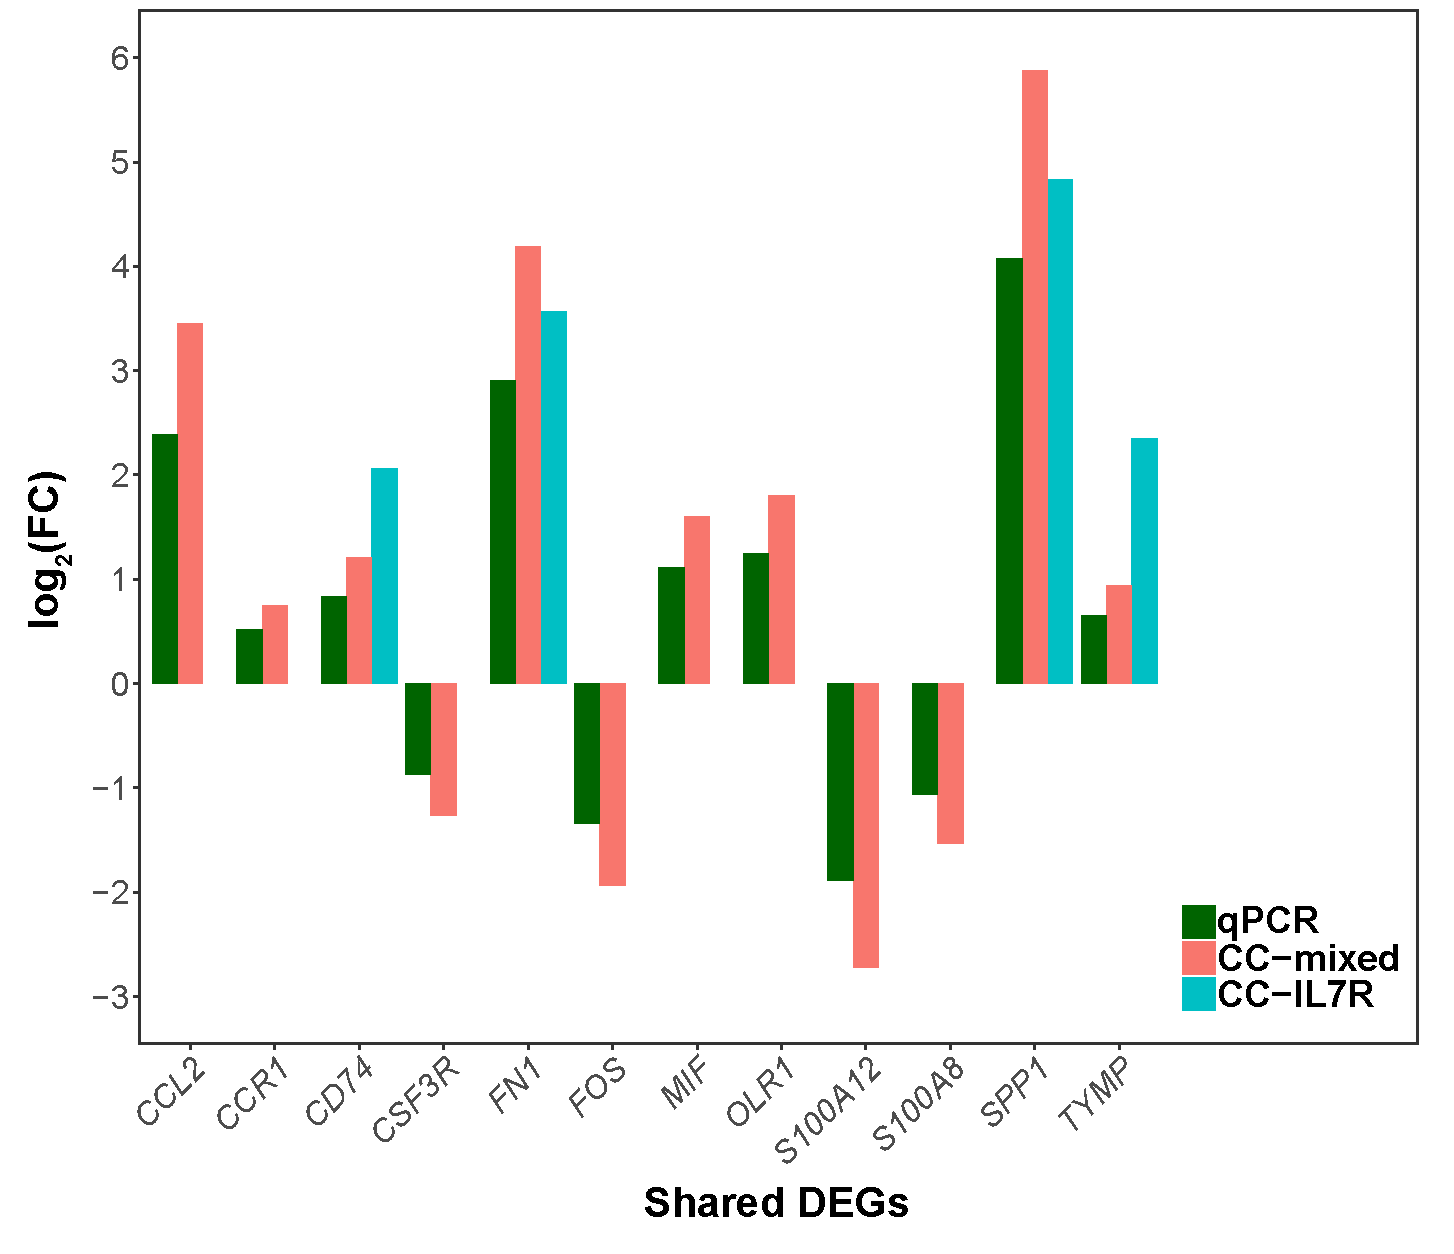
\includegraphics[width=\textwidth]{./Results3/pdfs/PSA_scRNAseq_PCR_array_overlapping_genes_log2FC}
\caption{}
\end{subfigure}
~
\begin{subfigure}[b]{0.70\textwidth} 
%the [b] prevents offset in subcaptions
\centering
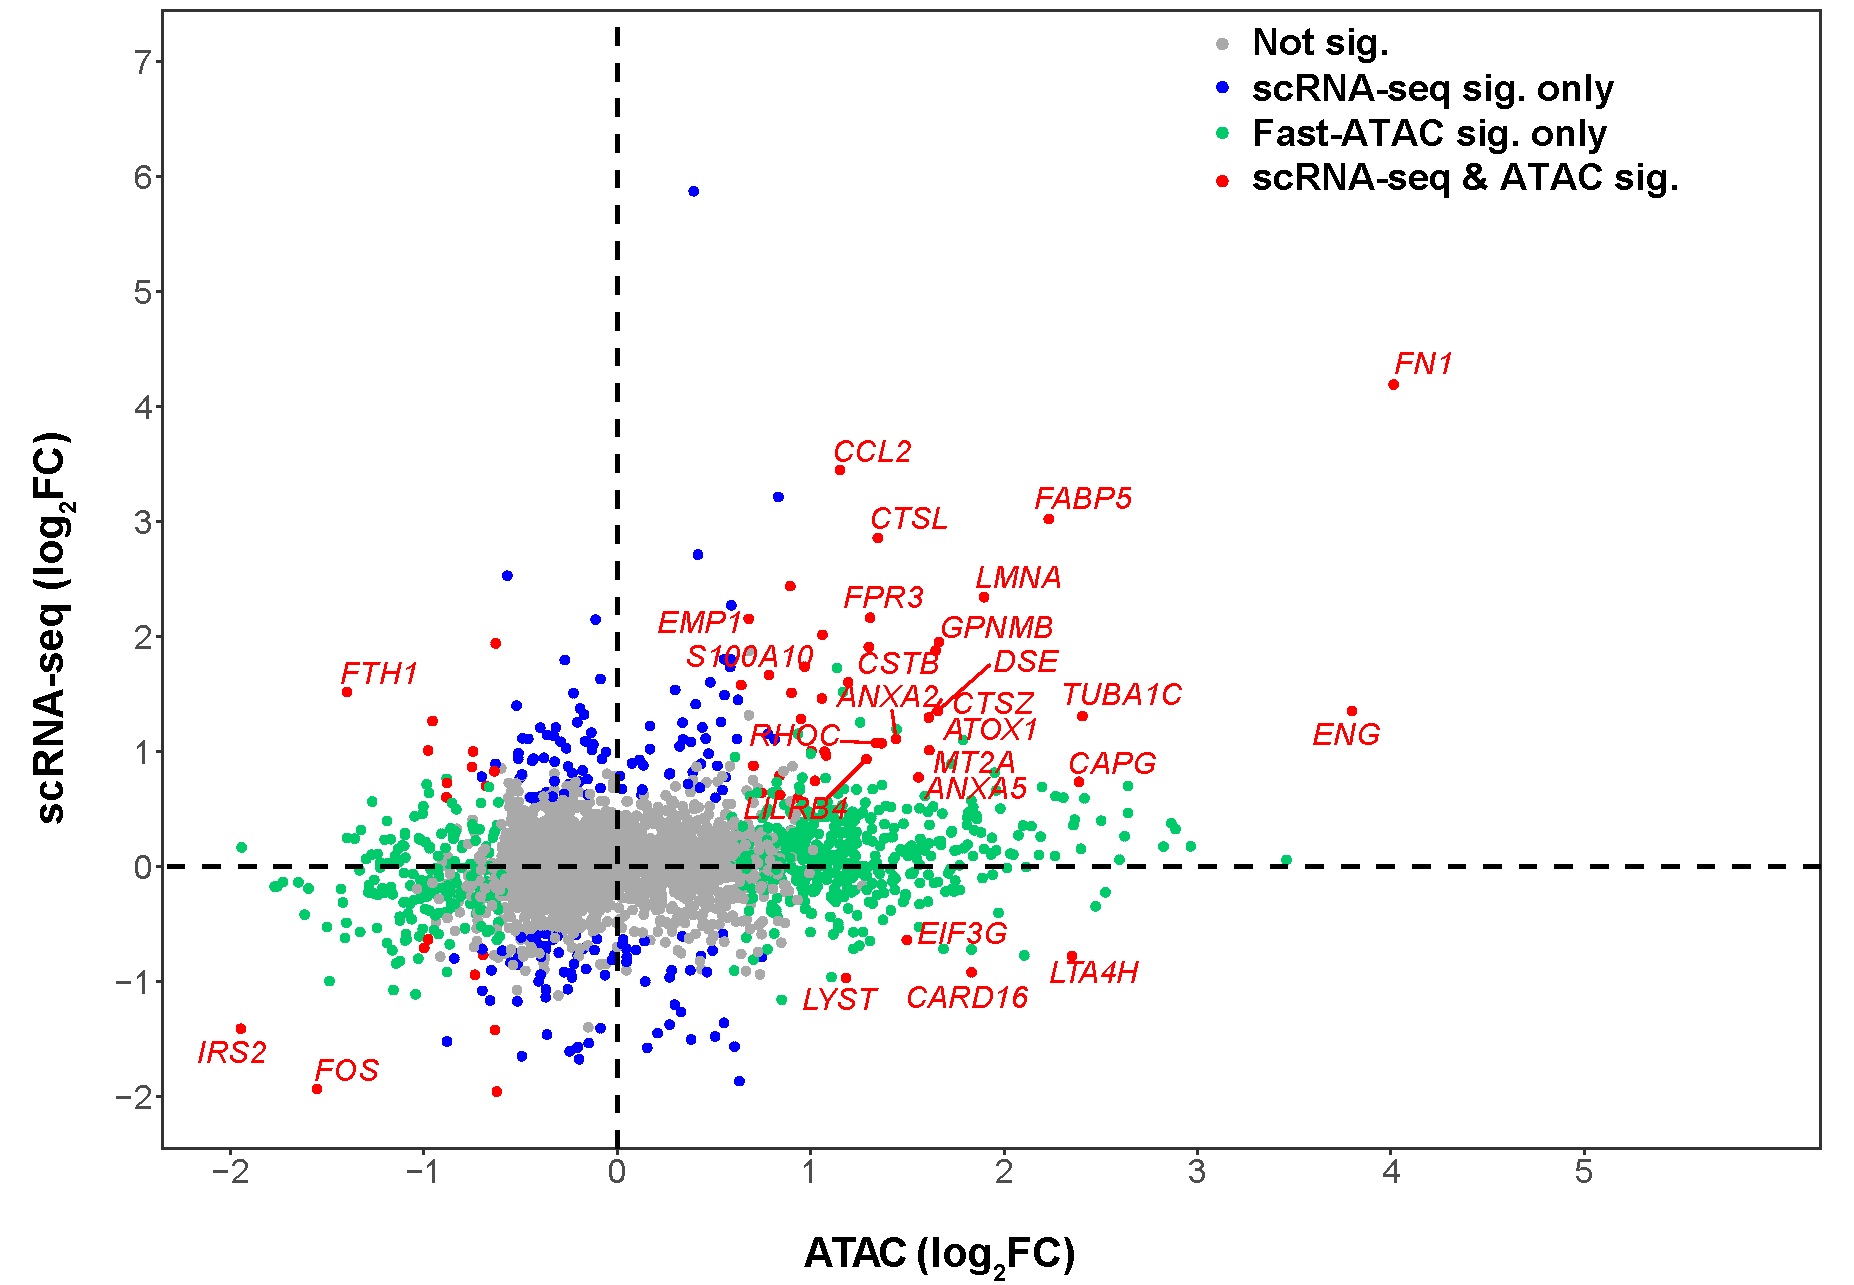
\includegraphics[width=\textwidth]{./Results3/pdfs/PSA_ATAC_scRNA_CD14_correlation_plot}
\caption{}
\end{subfigure}
\caption[Correlation between scRNA-seq, qPCR and chromatin accessibility in PsA CD14$^+$ monocytes.]{\textbf{Correlation between scRNA-seq, qPCR and chromatin accessibility in PsA CD14$^+$ monocytes.} a) Overlap between the scRNA-seq DEGs (significant based only on FDR$<$0.01) from the CC-mixed and CC-IL7R CD14$^+$ monocyte cluster in SF versus PB and the corresponding DEGs (pval<0.05) detected by qPCR in the bulk CD14$^+$ monocytes population. For each of the shared DEGs, the log$_2$FCs from the qPCR and the 10X scRNA-seq analysis are represented. b) Correlation between the 10X scRNA-seq gene expression in the CC-mixed CD14$^+$ monocytes cluster and the Fast-ATAC signal proximal to the same gene in total CD14$^+$ monocytes. Log$_2$FCs between SF and PB are represented for all the genes and Fast-ATAC regions included in the analysis and significance based on FDR and FC thresholds (FDR$<$0.01 and abs(FC)$>$1.5 in each of the assays is colour-coded.}
\label{figure:PsA_scRNAseq_qPCR_ATAC_correlation}
\end{figure}



%Interestingly, latest studies have involved RPS proteins in immune signalling and modulation of the NF-$\kapa$B response \parencite{Zhou2015}

\begin{table}[htbp]
%\setlength{\tabcolsep}{20pt} only to stretch the columns if you want
%\renewcommand{\arraystretch}{1.5}
\centering
\begin{tabular}{@{} c c c}
\toprule
\textbf{Cluster} & \textbf{Pathways} \\
\midrule
\midrule
         & Ag processing and presentation via MHC-II \\
				 & Extracellular matrix and extracellular \\
				 & matrix-associated proteins \\
CC-mixed & Phagosome and lysosome formation \\
				 & IFN signaling & \\
				 & Cytokine signalling $^\ast$ \\
				 & Apoptosis \\
				 & Innate immunity \\
\midrule				
         & Adaptive immunity \\
         & Ag processing and presentation \\
CC-IL7R	 & Phagosome \\
         & Extracellular matrix and extracellular \\
				 & matrix-associated proteins \\
\bottomrule
\end{tabular}
\medskip %gap
\caption[Most relevant enriched pathways for the DEGs between SF and PBCD14$^+$ monocytes in CC-mixed and CC-IL7R.]{\textbf{Most relevant enriched pathways for the DEGs between SF and PBCD14$^+$ monocytes in CC-mixed and CC-IL7R.} Significantly DEGs based on the FDR and FC threhold were used for the analysis. Most relevant enriched pathways based on FDR$<$0.01. ($\ast$) Enrichment for FDR$<$0.05.}
\label{tab:PSA_scRNAseq_CD14_DEGs_pathway_analysis}
\end{table}


\subsubsection{Moderate genome-wide correlation correlation between chromatin accessibility and scRNA-seq expression in the CC-mixed cluster }
In order to determine the overall correlation between expression and chromatin accessibility, the log$_2$FCs for all the expressed genes in the CC-mixed CD14$^+$ monocytes cluster and all the accessible chromatin regions in total CD14$^+$ monocytes between SF and PB were compared (Figure \ref{figure:PsA_scRNAseq_qPCR_ATAC_correlation} b). Changes in expression and chromatin accessibility only presented a moderate correlation in this data (R$^2$=0.214, pval=2x10$^{-16}$). In the CC-mixed cluster, 64 genes out of the 251 DEGs (FDR$<$0.01 and abs(FC)$>$1.5) were nearby one or more Fast-ATAC DARs (Table \ref{tab:PSA_10X_CD14_clusters_and_ATAC_overlap}). Interestingly, the CC-mixed DEGs were enriched for genes in the proximity of at least one DARs in total CD14$^+$ monocytes (Fisher exact test pval=1.5x10$^-3$) highlighting a mechanistic effect???. The majority of the overlaps presented corresponding up-regulation or down-regulation (40 and 12 genes, respectively)in both, gene expression and chromatin accessibility, when comparing SF versus PB. However, 12 genes showed opposite dysregulated expression and chromatin accessibility in the CC-mixed cluster (Table \ref{tab:PSA_10X_CD14_clusters_and_ATAC_overlap}). 


  
\begin{table}[htbp]
%\setlength{\tabcolsep}{20pt} only to stretch the columns if you want
%\renewcommand{\arraystretch}{1.5}
\centering
\begin{tabular}{@{} c c c c}
\toprule
\textbf{Cluster} & \textbf{Up-regulated genes}        &  \textbf{Up-regulated genes }  & \textbf{Opposite direction} \\
                   & \textbf{with proximal}           &  \textbf{with proximal}      & \textbf{in expression } \\
									 &	\textbf{SF open DAR}				    &  \textbf{PB open DAR}        & \textbf{and DAR}\\
\midrule
\midrule
 CC-mixed         & 40                                       &  10                                & 14 \\
 CC-IL7R          & 9                                        &  0                                 & 4 \\
\bottomrule
\end{tabular}
\medskip %gap
\caption[scRNA-seq DEGs in SF versus PB CD14$^+$ monocytes proximal to a DAR in Fast-ATAC.]{\textbf{scRNA-seq DEGs in SF versus PB CD14$^+$ monocytes proximal to a DAR in Fast-ATAC.}. For each of the two CD14$^+$ monocytes cluster identified by scRNA-seq analysis, an overlap is defined by significant change in expression (FDR$<$0.01 and abs(FC)$>$1.5) between SF and PB for a particular gene where a proximal DAR ($\leq$5Kb) showing same or opposite direction of change to the gene expression.}
\label{tab:PSA_10X_CD14_clusters_and_ATAC_overlap}
\end{table}


Interestingly, amongst the DEGs in the CC-mixed cluster overlapping a proximal DAR was \textit{CCL2} (Figure \ref{figure:PsA_scRNAseq_qPCR_ATAC_correlation} b). The expression of \textit{CCL2} was shown to be significantly modulated (pval$<$0.05 and mean FC$>$1.5) between SF and PB by qPCR only in CD14$^+$ monocytes, whereas no significant changes were observed for mCD4$^+$ and mCD8$^+$ in the same data (Figure \ref{figure:PSA_PCR_array_vulcano_plots} a, b, c and Table \ref{tab:PSA_gene_expression_ATAC_overlap}). In contrast, \textit{CCR2} which is the receptor for the chemokine MCP-1 (protein product of \textit{CCL2}) appeared up-regulated in mCD4$^+$ and mCD8$^+$ cells in the same individuals, highlighting the biological relevance of this observation. Consistently with \textit{CCL2} up-regulated expression in SF compared to PB was, a cell type-specific SF open DAR upstream \textit{CCL2} has also been identified by Fast-ATAC in this data (Figure \ref{figure:PsA_10X_qPCR_ATAC_CD14_CCL2}). This SF open DAR region is annotated as enhancer according to Epigenome Roadmap chromatin segmentation and overlaps a eRNA reported by FANTOM5 in CD14$^+$ monocytes. However, no eQTL or Hi-C interaction in CD14$^+$ monocytes have been reported for SNPs overlapping this DAR, lacking of additional data to determine the relationship between differential expression of \textit{CCL2} and changes in chromatin accessibility in this nearby locus. In terms of the pathological relevance, \textit{CCL2} did not appear up-regulated in PB CD14$^+$ monocytes when comparing PsA patients and healthy controls and it was defined as one of the putative disease-specific genes (Figure \ref{figure:figure:PSA_PCR_array_HC_FC_correlation} a). Similarly, Dolcino and colleagues were not able to detect \textit{CCL2} dysregulation neither in PBMCs when comparing PsA patients and healthy controls nor when comparing synovial membrane biopsies from PsA patients versus controls \parencite{Dolcino2015}. Overall, this suggests a tissue and cell type specific dysregulation of \textit{CCL2} expression in the CC-mixed CD14$^+$ monocytes cluster that may be related to alterations in the chromatin accessibility of an enhancer in the proximity to this gene.

\bigskip
\begin{figure}[H]
\centering
\begin{subfigure}[b]{0.60\textwidth}
\centering 
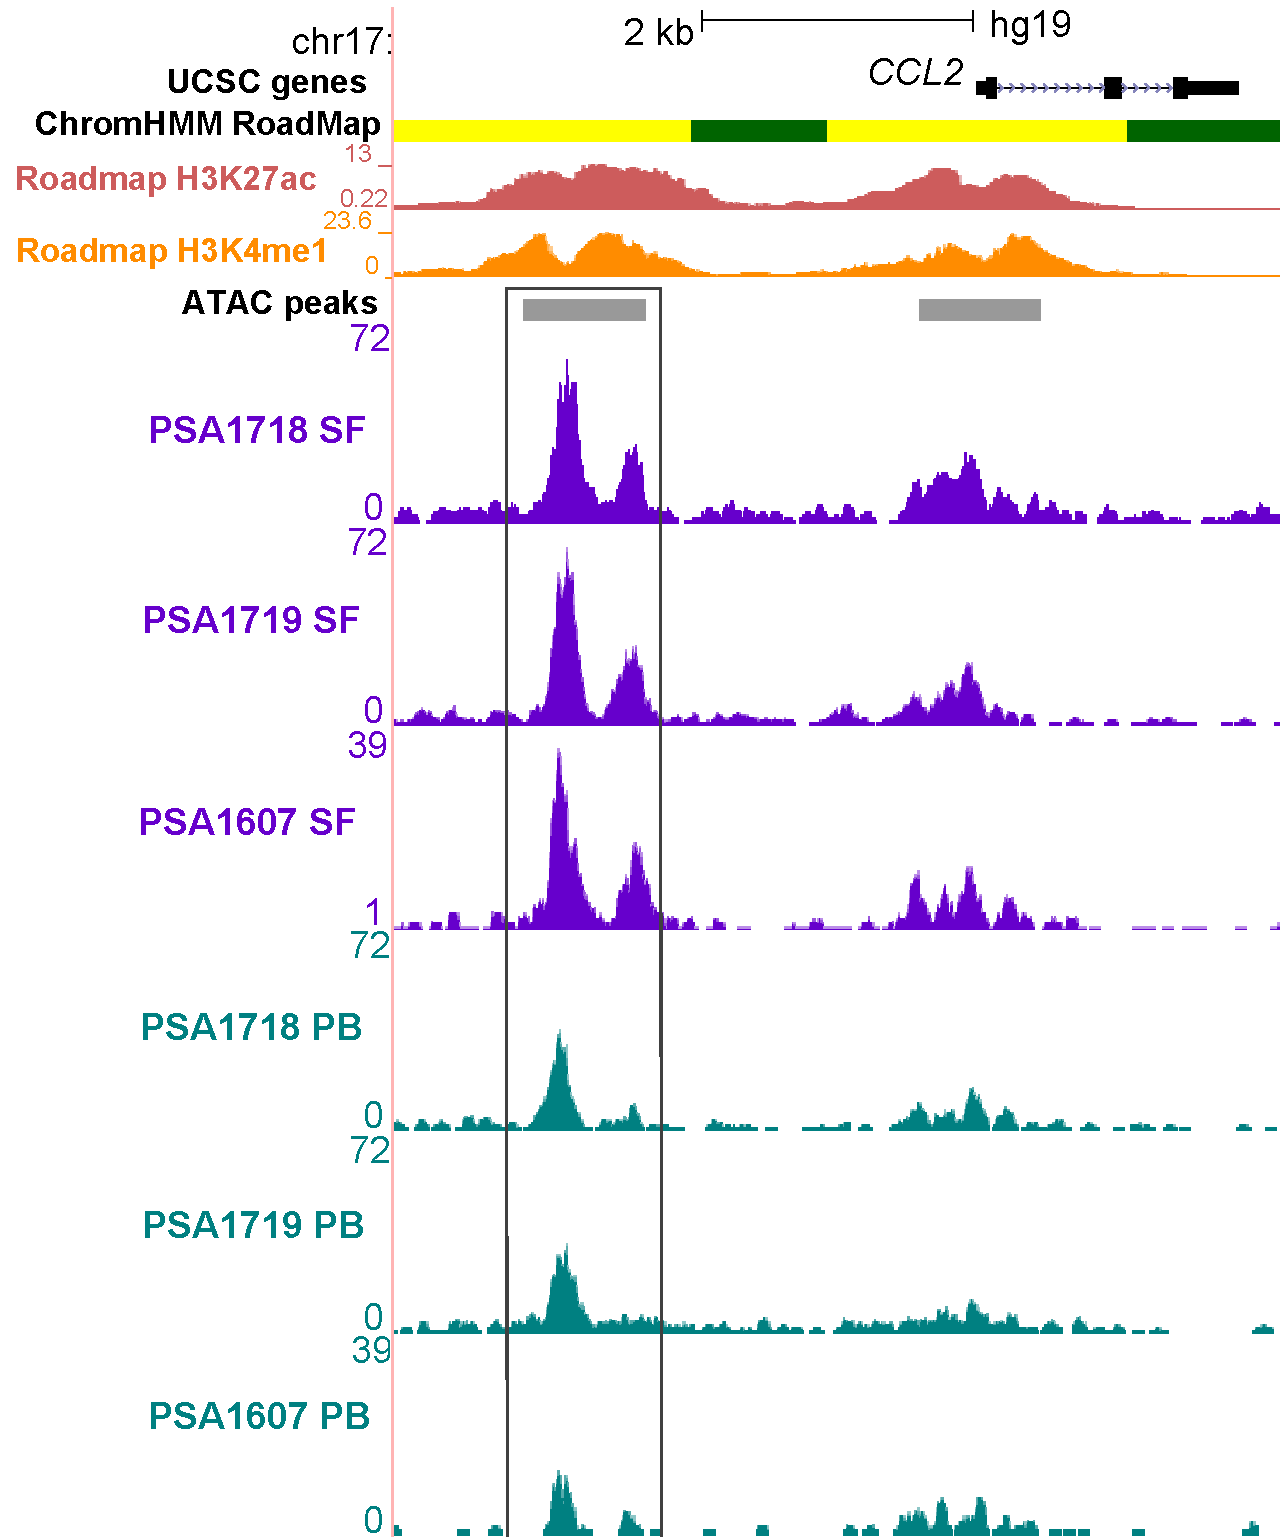
\includegraphics[width=\textwidth]{./Results3/pdfs/ATAC_PSA_CD14_UCSC_CCL2_track}
\caption{}
\end{subfigure}
\caption[Differentially accessible regions located within gene bodies in CD14$^+$ monocytes and NK cells from PsA patients.]{\textbf{Differentially accessible regions located within gene bodies in CD14$^+$ monocytes and NK cells from PsA patients.} xxxx}
\label{figure:PsA_10X_qPCR_ATAC_CD14_CCL2}
\end{figure}


Similarly to the CC-mixed results, the DEGs in the CC-IL7R cluster between SF and PB were also enriched for those genes with at least one DARs nearby (Fisher exact test pval=1.85x10$^-9$). Amongst the 22 DEGs overlapping a proximal DAR, 13 of them had gene expression and chromatin accessibility changing in the same direction and only 4 presented opposite directionality in the variation of the two features (Table \ref{tab:PSA_10X_CD14_clusters_and_ATAC_overlap}). The CC-IL7R cluster and CD44 data not shown.
% Only row avg expression or chr accessibility in each tissue, in case there is a better correlation in one compared to the other
%Do fisher exact for DEGs and ATAC but also see relationship with cell type specific genes and tissue specific genes, to try to merge everything, or establish one link/conclusion or finding




%The biological relevance of the IL7R does not show distinct differences in gene expression between tissues and its relevance may be related to the distinctive biological function of this subset in both tissues. Seems more abundant in SF and that would make sense with the differences in the PCR array in bulk expression.




\subsection{Mass cytometry reveals CD14$^+$ monocytes as the most active cytokine producing cells}
%Maybe see if adding a figure of the clusters and the main markers to complement
Measurement of cytokine production using mass cytometry was conducted in collaboration with Dr Hussein Al-Mossawi and Dr Nicole Yager. Cytokine production by CD14$^+$ monocytes, mCD4$^+$ T cells, mCD8$^+$ T cells and NK was quantified in SF and PB after incubation with BFA for 6 h. BFA blocks cytokine release and enables to measure the cell cytokine production rate in absence of any inflammatory stimuli, as previously explained in Chapter \ref{ch:Mat}(Figure \ref{figure:PSA_cytof_cytokines}). Following data QC, IL-2, IL-8, IFN-$\gamma$ and TNF-$\alpha$ were the cytokines consistently released with the most reliable quantification results within each of the manual gated cell type clusters. CD14$^+$ monocytes isolated from both, SF and PB, was the only active cell type in producing IFN-$\gamma$, IL-2 and IL-8. Nevertheless, no significant differences in the production (mean) of those three cytokines was observed in CD14$^+$ monocytes between SF and PB. On the other hand, only CD14$^+$ monocytes isolated from SF showed positive detectable mean levels of TNF-$\alpha$, which was undetectable in the PB counterpart cells. 

% IL8 production in CD4 https://www.ncbi.nlm.nih.gov/pubmed/7763239
% IL-8 monocytes and other cell types https://www.ncbi.nlm.nih.gov/pmc/articles/PMC4188125/
% TNFa in CD8 http://www.reproduction-online.org/content/141/2/249.full
\begin{figure}[htbp]
\centering
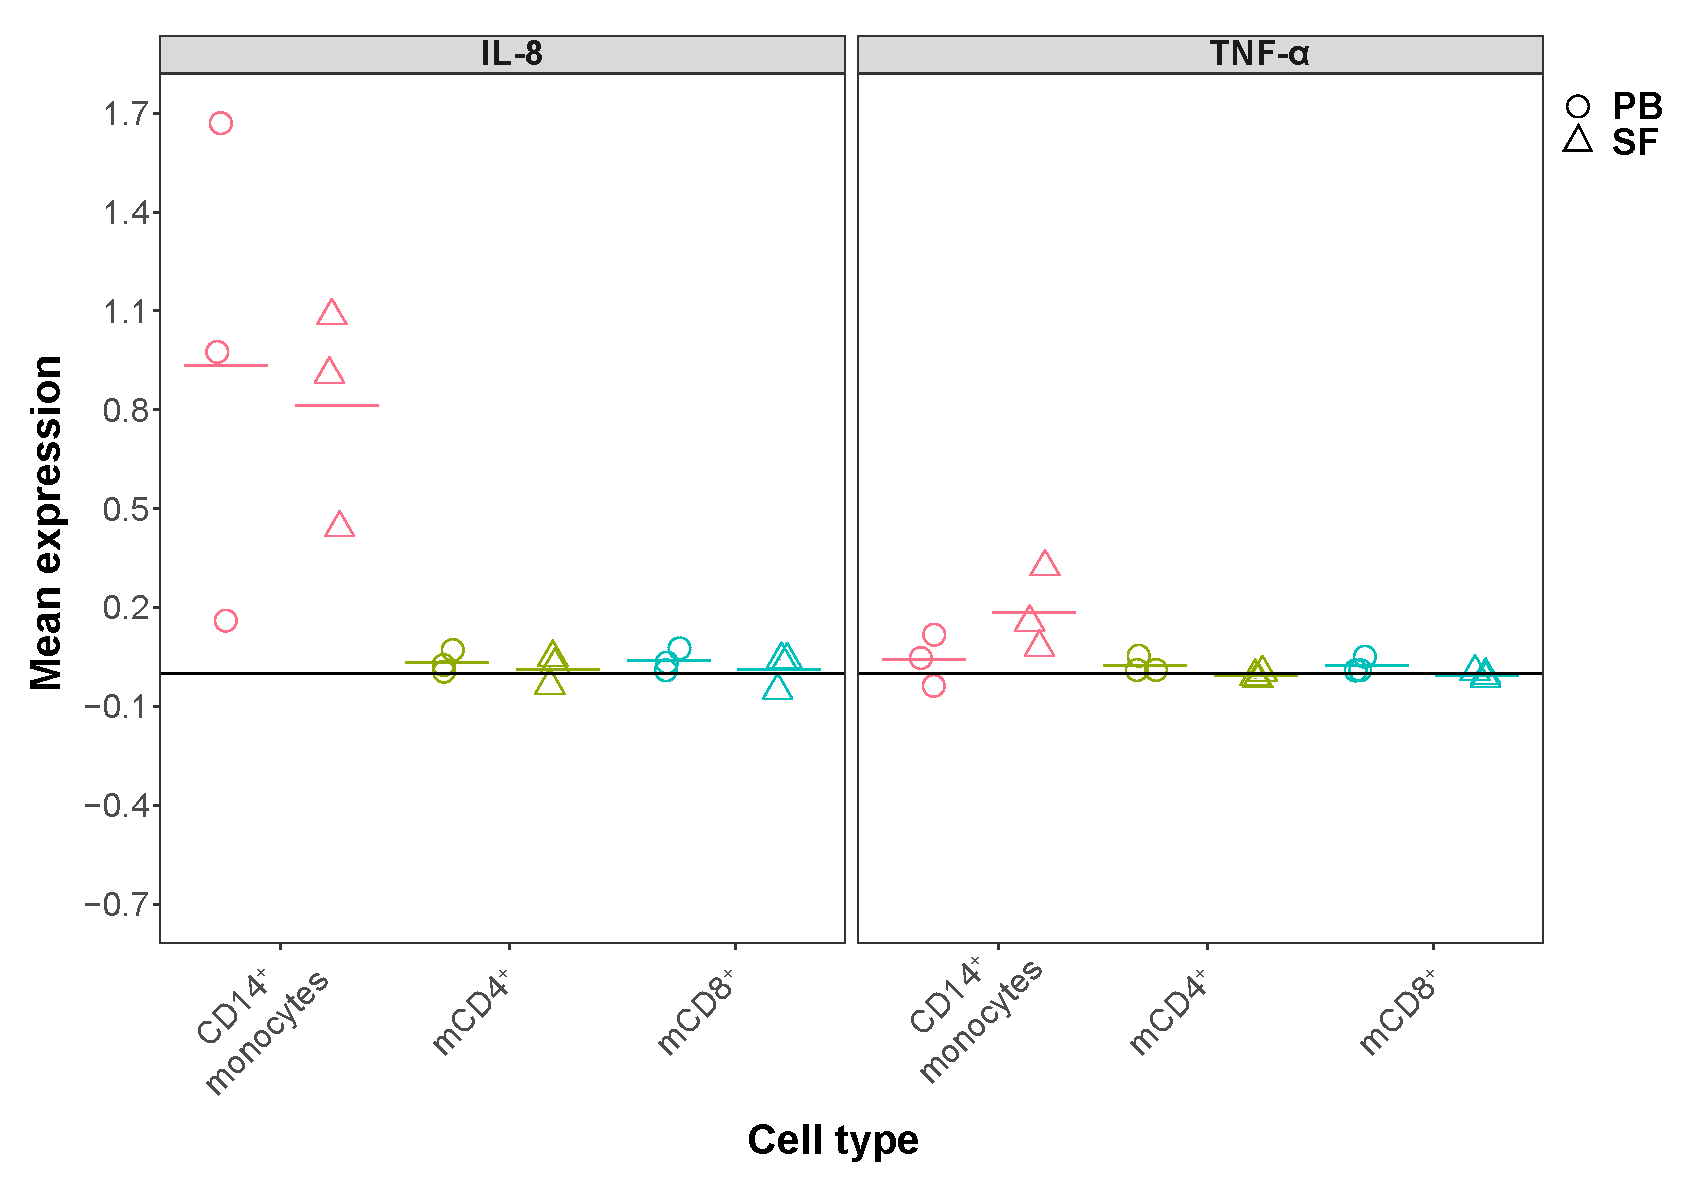
\includegraphics[width=0.6\textwidth]{./Results3/pdfs/CyTOF_ICS_cytokines_production_IL8_TNF}
\caption[Mean expression of IL-8 and TNF-$\alpha$ in SF and PB from PsA patients.]{\textbf{Mean expression of IL-8 and TNF-$\alpha$ in SF and PB from PsA patients.} Expression levels quantified by mass cytometry. xxxx }
\label{figure:PSA_cytof_cytokines}
\end{figure}


The increased rate of TNF-$\alpha$ production by SF CD14$^+$ monocytes was reinforced when comparing the proportion of TNF-$\alpha$ positive cells after 6h of blocked cytokine secretion in each of the two tissues. The mass cytometry analysis of CD14$^+$ versus TNF-$\alpha$ signal showed a greater number of SF CD14$^+$ monocytes producing TNF$\alpha$ after 6 h of BFA treatment compared to PB for each of the three analysed patients (Figure \ref{figure:PsA_monocytes_percentage_TNFa} a). The basal (0h) percentage of CD14$^+$ monocytes positive for TNF-$\alpha$was negligible for all three patients in both, SF and PB (Figure \ref{figure:PsA_monocytes_percentage_TNFa} b). Conversely, upon inhibition of protein transport (6h), the percentage of CD14$^+$ monocytes producing TNF-$\alpha$ experienced an increase, ranging between 2 and 11.8\%, in SF whereas the increment in PB did not reach 1\%. This trend of increased percentage of SF CD14$^+$ monocytes TNF-$\alpha$ did not reach significance likely due to the small sample size. 
 
\bigskip
\begin{figure}[H]
\centering
\begin{subfigure}[b]{0.80\textwidth}
\centering 
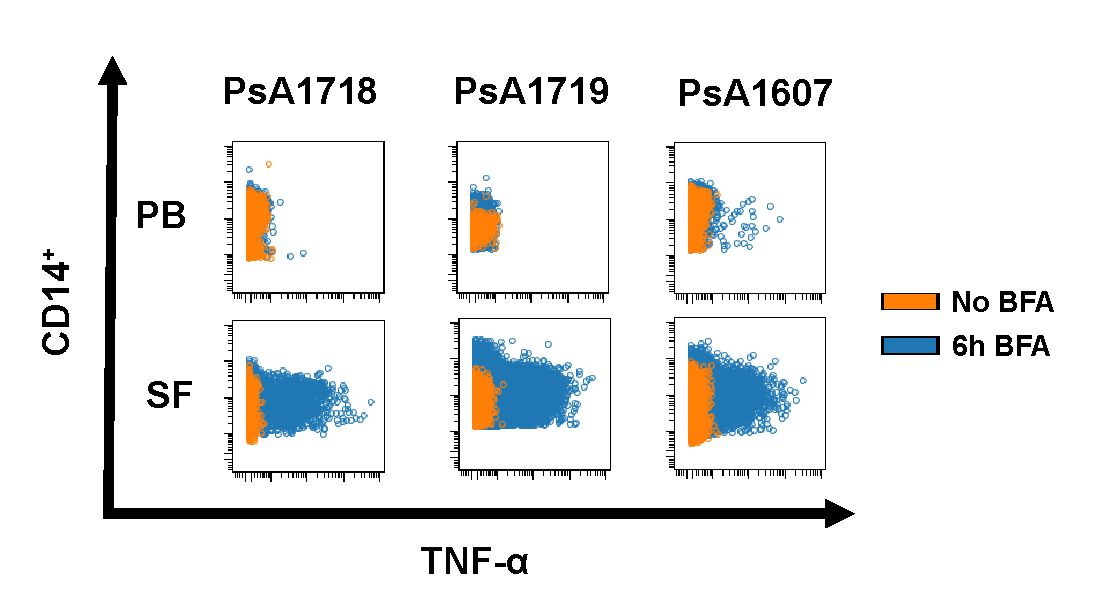
\includegraphics[width=\textwidth]{./Results3/pdfs/PSA_0h_6h_BFA_TNFa_mass_cytometry_PSA1718_PSA1719_PSA1607}
\caption{}
\end{subfigure}
~
\begin{subfigure}[b]{0.65\textwidth} 
%the [b] prevents offset in subcaptions
\centering
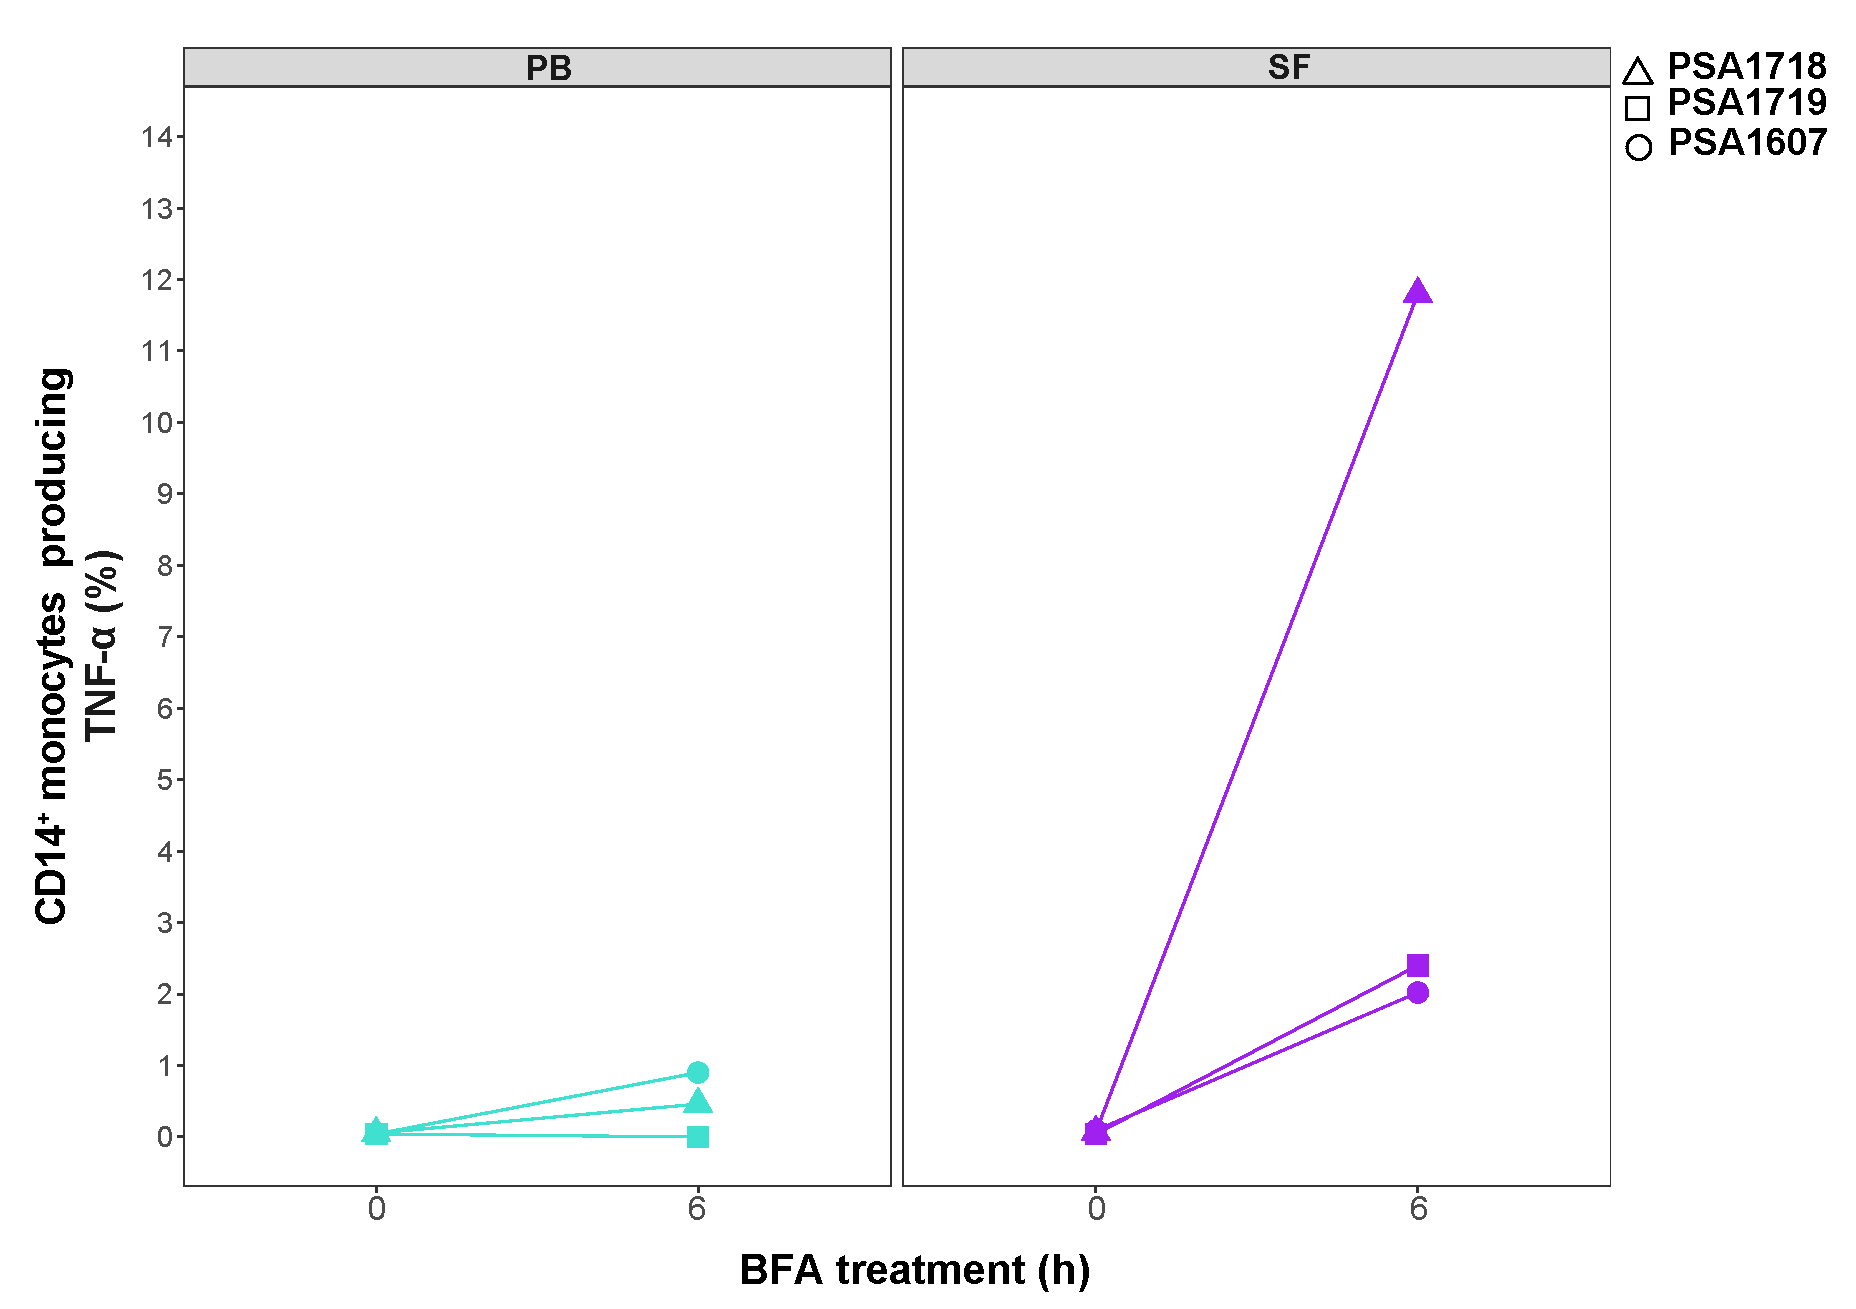
\includegraphics[width=\textwidth]{./Results3/pdfs/PSA_percent_monocytes_producing_TNFa_PB_and_SF}
\caption{}
\end{subfigure}
\caption[Mass cytometry analysis of TNF-$\alpha$ production in SF and PB by CD14$^+$ monocytes after protein transport blockade with BFA.]{\textbf{Differentially accessible regions located within gene bodies in CD14$^+$ monocytes and NK cells from PsA patients.} xxxx}
\label{figure:PsA_monocytes_percentage_TNFa}
\end{figure}


%This cytokine panel is representative of the four cell types of interest. TNF-$\alpha$ is released by all four cell types whereas IFN-$\gamma$ is mostly produced by lymphocytes and NK cells. Although IL-8 is mainly produced by fibroblasts and neutrophils, it is also secreted by monocytes and CD4$^+$ T cells, this last one being also the main source for IL-2 production. 


\subsection{Integration of PsA GWAS and epigenetics}

ATAC peaks overlap with GWAS
DEGs in PCR array or scRNA with GWAS
Fine-mapping of those loci
%%%%%%
% Fig is the pb and sf populations together with the following markers




%%%%%%%%%%%%%%%%%%%%%%%%%%%%%%%%%%%%%%%%%%%%%%%%%%
\section{Discussion}
%
In Dolcino PSA vs HV SF comparison also detected more up genes than down in the array analysis
Say which cell types drive more the top changed gened

fGWAS analysis as Matthias did would be of interest but needs appropriate GWAS data
I am going to try using XGR to do some of this 

%NOD-like in PsA: https://www.ncbi.nlm.nih.gov/pmc/articles/PMC4792137/
%TLR in PsA: https://www.ncbi.nlm.nih.gov/pmc/articles/PMC2787278/

% SIGRR downregulation by LPS https://www.ncbi.nlm.nih.gov/pmc/articles/PMC4140261/
% CCL2 and CXCL10 in PsA

The integration of the varied types of datasets that can be generated from clinical samples of a wide range of complex diseases remains challenging. It requires the implementation or development of new algorithms in order to integrate them into a systematic way
Machine learning has been used for RA https://onlinelibrary.wiley.com/doi/epdf/10.1002/art.40428
CCA analysis also for RA Zhang2018	


%Regarding the low number of qPCR DEGs between SF and PB in total CD14$^+$ monocytes reproduced by the scRNA-seq in any of the two main clusters identified could be explained by the differences in the cell sorting (FACS versus \textit{in silico} expression markers), the low number of replicates for each assay as well as different sensitivity of the two technologies.   
